\chapter{Números e mais números}
\markboth{Módulo 1}{}

\coment{Habilidades da BNCC: EF05MA01, EF05MA10, EF05MA11.}

\colorsec{Habilidades do SAEB}

\begin{itemize}
\item Escrever números racionais (naturais de até 6 ordens, representação
fracionária ou decimal finita até a ordem dos milésimos) em sua
representação por algarismos ou em língua materna ou associar o registro
numérico ao registro em língua materna.

\item Identificar a ordem ocupada por um algarismo ou seu valor posicional
(ou valor relativo) em um número natural de até 6 ordens.

\item Comparar ou ordenar números racionais (naturais de até 6 ordens,
representação fracionária ou decimal finita até a ordem dos milésimos),
com ou sem suporte da reta numérica.

\item Compor ou decompor números naturais de até 6 ordens na forma aditiva,
ou em suas ordens, ou em adições e multiplicações.

\item Comparar diferentes sentenças de adições ou de subtrações de dois números naturais.

\item Determinar o número desconhecido que torna verdadeira uma igualdade
que envolve as operações fundamentais com números naturais de até 6
ordens.
\end{itemize}

\conteudo{Professor, neste módulo devemos revisar os conceitos de montagem de
números, frisando muito as classes e até a 6º ordem. É muito importante
os alunos finalizarem o módulo sabendo o valor posicional e relativo de
cada algarismo quando estão em determinada ordem.

Além disso, deve-se trabalhar minuciosamente a decomposição dos números e sua
escrita por extenso.

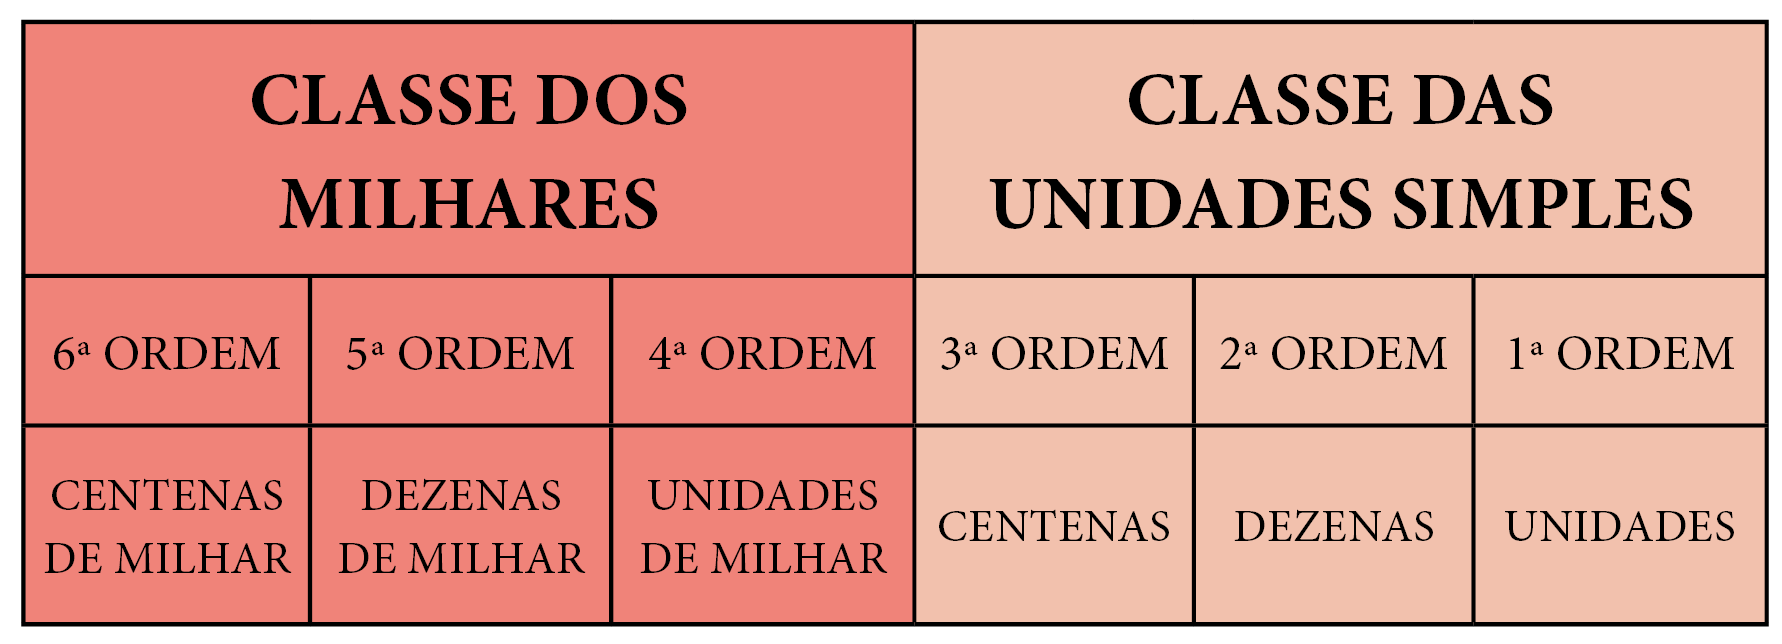
\includegraphics[width=\textwidth]{../ilustracoes/MAT5/SAEB_5ANO_MAT_figura1.png}

Valor posicional ou relativo: é o valor que o algarismo assume dependendo da classe e da ordem em que ele está posicionado no número.

Exemplo: No número 352.146, o algarismo 5 possui valor posicional ou
relativo igual a 50.000, pois ocupa a 5º ordem, a qual está dentro da
classe dos milhares, ou seja, está na posição da dezena de milhar; sendo
assim, 5 x 10.000 = 50.000.}

\colorsec{Atividades}

\num{1} Escreva dentro dos retângulos o valor posicional dos algarismos
destacados, ou seja, o valor que eles assumem de acordo com a posição que ocupam no número.

\begin{figure}[htpb!]

\includegraphics[width=.5\textwidth]{../ilustracoes/MAT5/SAEB_5ANO_MAT_figura2.png}
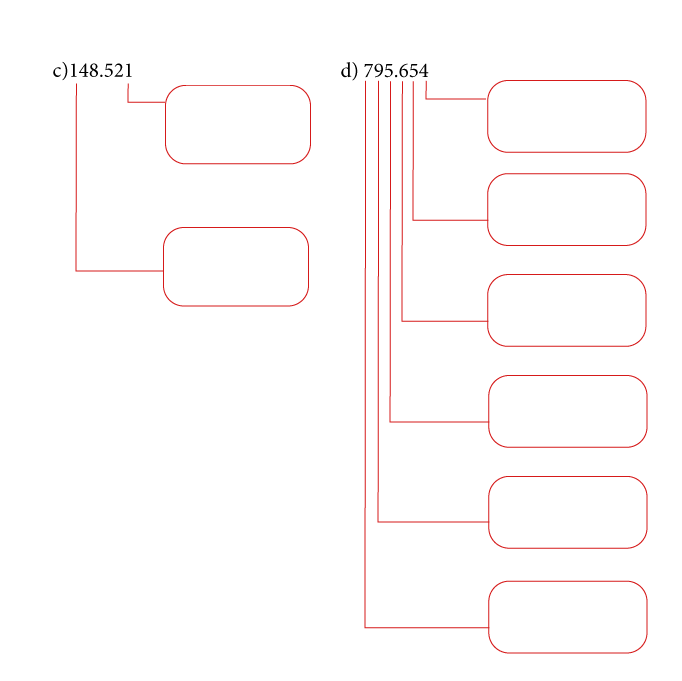
\includegraphics[width=.5\textwidth]{../ilustracoes/MAT5/SAEB_5ANO_MAT_figura2b.png}
\end{figure}

\coment{
a) O algarismo 8 destacado tem valor posicional igual a 800.000 (oitocentos mil), já que se encontra na centena de milhar.
b)  O primeiro algarismo 7 destacado tem valor posicional igual a 70.000 (setenta mil), já que se encontra na dezena de milhar.
Já o segundo algarismo 7 destacado tem valor posicional igual a 70 (setenta), já que está posicionado na dezena comum.
c)  O primeiro algarismo 1 destacado tem valor posicional igual a 100.000
  (cem mil), já que se encontra na centena de milhar.
Já o segundo algarismo 1 destacado tem o valor posicional igual a 1 (uma
unidade), já que se encontra na unidade comum.
d) O algarismo 7 destacado tem valor posicional igual a 700.000
  (setecentos mil), já que está na centena de milhar.
O algarismo 9 destacado tem valor posicional igual a 90.000 (noventa
mil), já que está na dezena de milhar.
O primeiro algarismo 5 destacado tem valor posicional igual a 5.000
(cinco mil), já que está na unidade de milhar.
O algarismo 6 destacado tem valor posicional igual a 600 (seiscentos), já
que está na centena comum.
O segundo algarismo 5 destacado tem valor posicional igual a 50
(cinquenta), já que está na dezena comum.
O algarismo 4 destacado tem valor posicional igual a 4 (4 unidades), já
que está na unidade comum.}

\num{2} Decomponha os números a seguir de acordo com o valor posicional de
cada algarismo.

\begin{escolha}
\item 32.084

\reduline{30.000 + 2.000 + 80 + 4 ou 3 x 10.000 + 2 x 1.000 + 0 x 100 + 8 x 10 + 4.\hfill}

\item 26.587

\reduline{20.000 + 6.000 + 500 + 80 + 7 ou 2 x 10.000 + 6 x 1.000 + 5 x 100 + 8 x 10 + 7.\hfill}

\item 2.105

\reduline{2.000 + 100 + 5 ou 2 x 1.000 + 1 x 100 + 0 x 10 + 5.\hfill}
\end{escolha}

\coment{Além disso, utilize o exercício para treinar a escrita dos alunos. Exemplo: trinta e dois mil e
oitenta e quatro.}

\num{3} Monte os números compostos e registre-os nos locais correspondentes.

\begin{escolha}
\item 7 unidades de milhar, 5 centenas e 4 unidades: \reduline{7.504.}

\item 3 dezenas de milhar, 7 dezenas e 2 unidades: \reduline{30.072.}

\item 9 centenas de milhar, 5 unidades de milhar e 6 centenas: \reduline{905.600.}

\item 2 unidades de milhar, 6 centenas e 3 unidades: \reduline{2.603.}
\end{escolha}

\coment{Professor, devemos explorar bem a escrita dos números a partir da decomposição, pois muitos alunos desenvolvem
dificuldades, conseguindo fazer a decomposição, mas sem compreender a volta (montagem dos números decompostos).}

\num{4} Ligue os retângulos da coluna com 1 a um corresponde da coluna 2
que represente a escrita por extenso do número indicado na primeira
coluna.

\begin{figure}[htpb!]
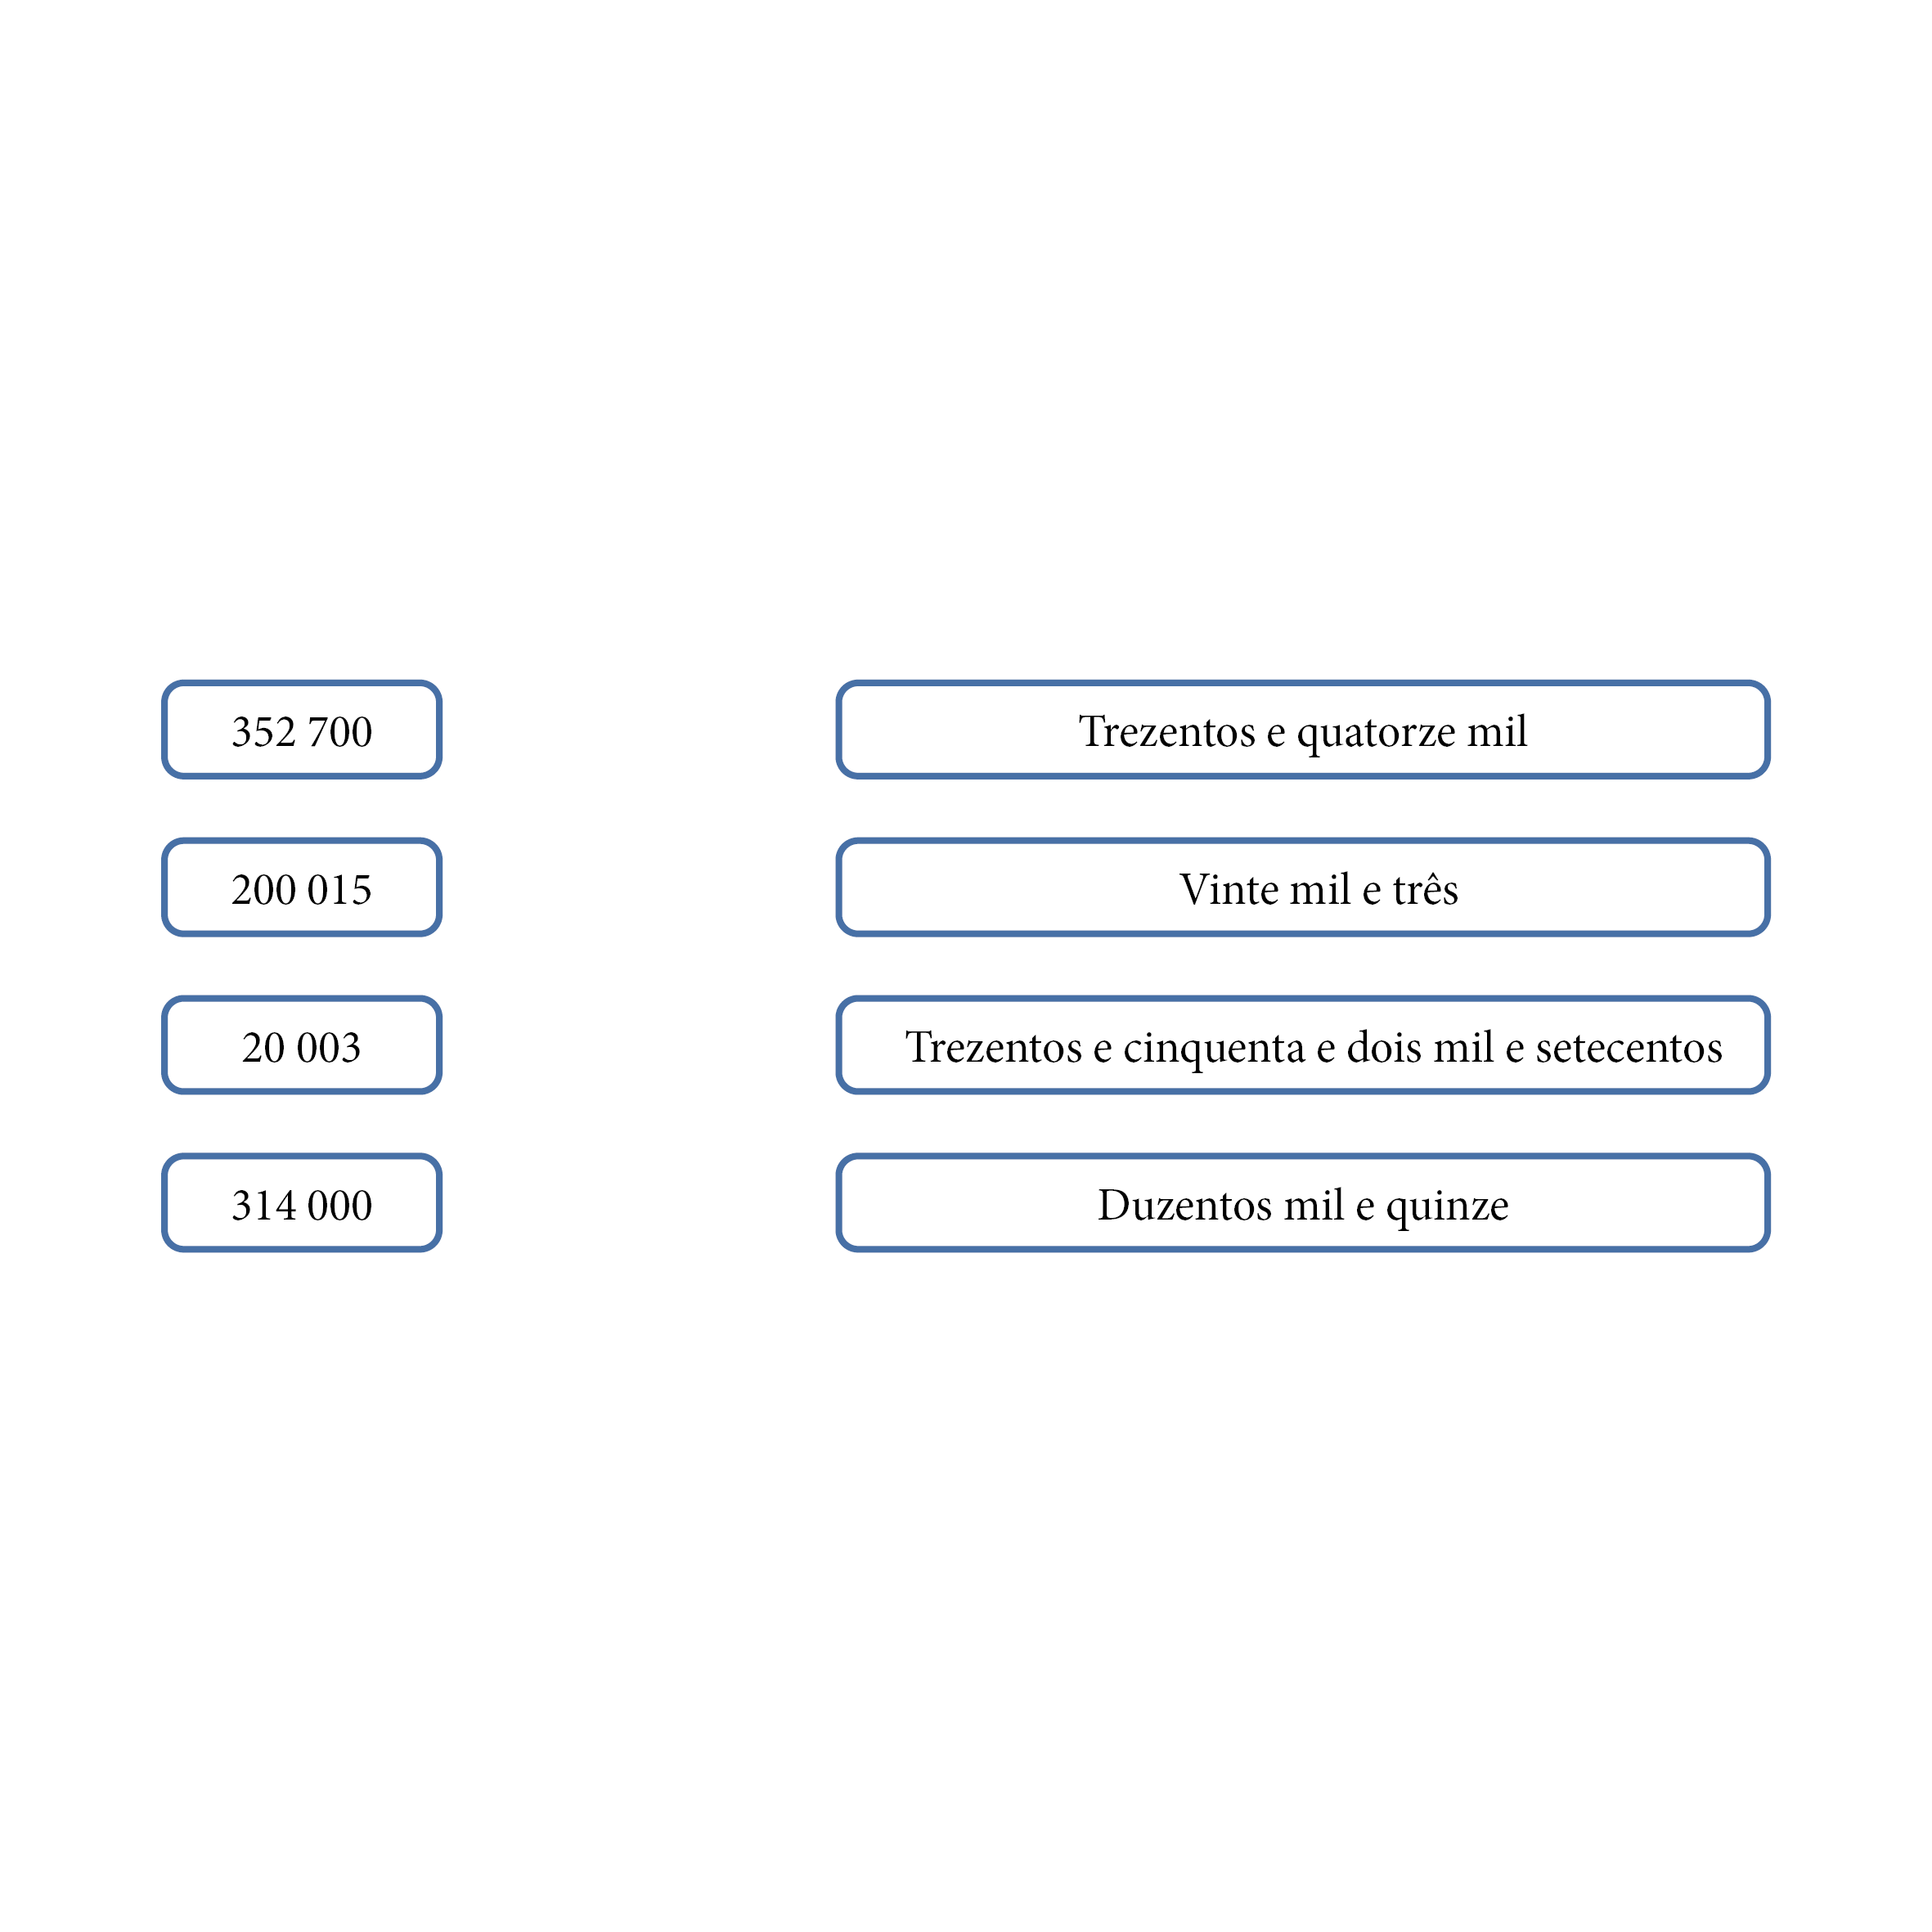
\includegraphics[width=\textwidth]{../ilustracoes/MAT5/SAEB_5ANO_MAT_figura3.png}
\end{figure}

\coment{
352.700 deve estar ligado a “trezentos e cinquenta e dois mil e setecentos”.
200.015 deve estar ligado a “duzentos mil e quinze”.
20.003 deve estar ligado a “vinte mil e três”.
314.000 deve estar ligado a “trezentos e catorze mil”.}

\num{5} Utilizando o material dourado, Ana Letícia montou o seguinte número:

\begin{figure}[htpb!]
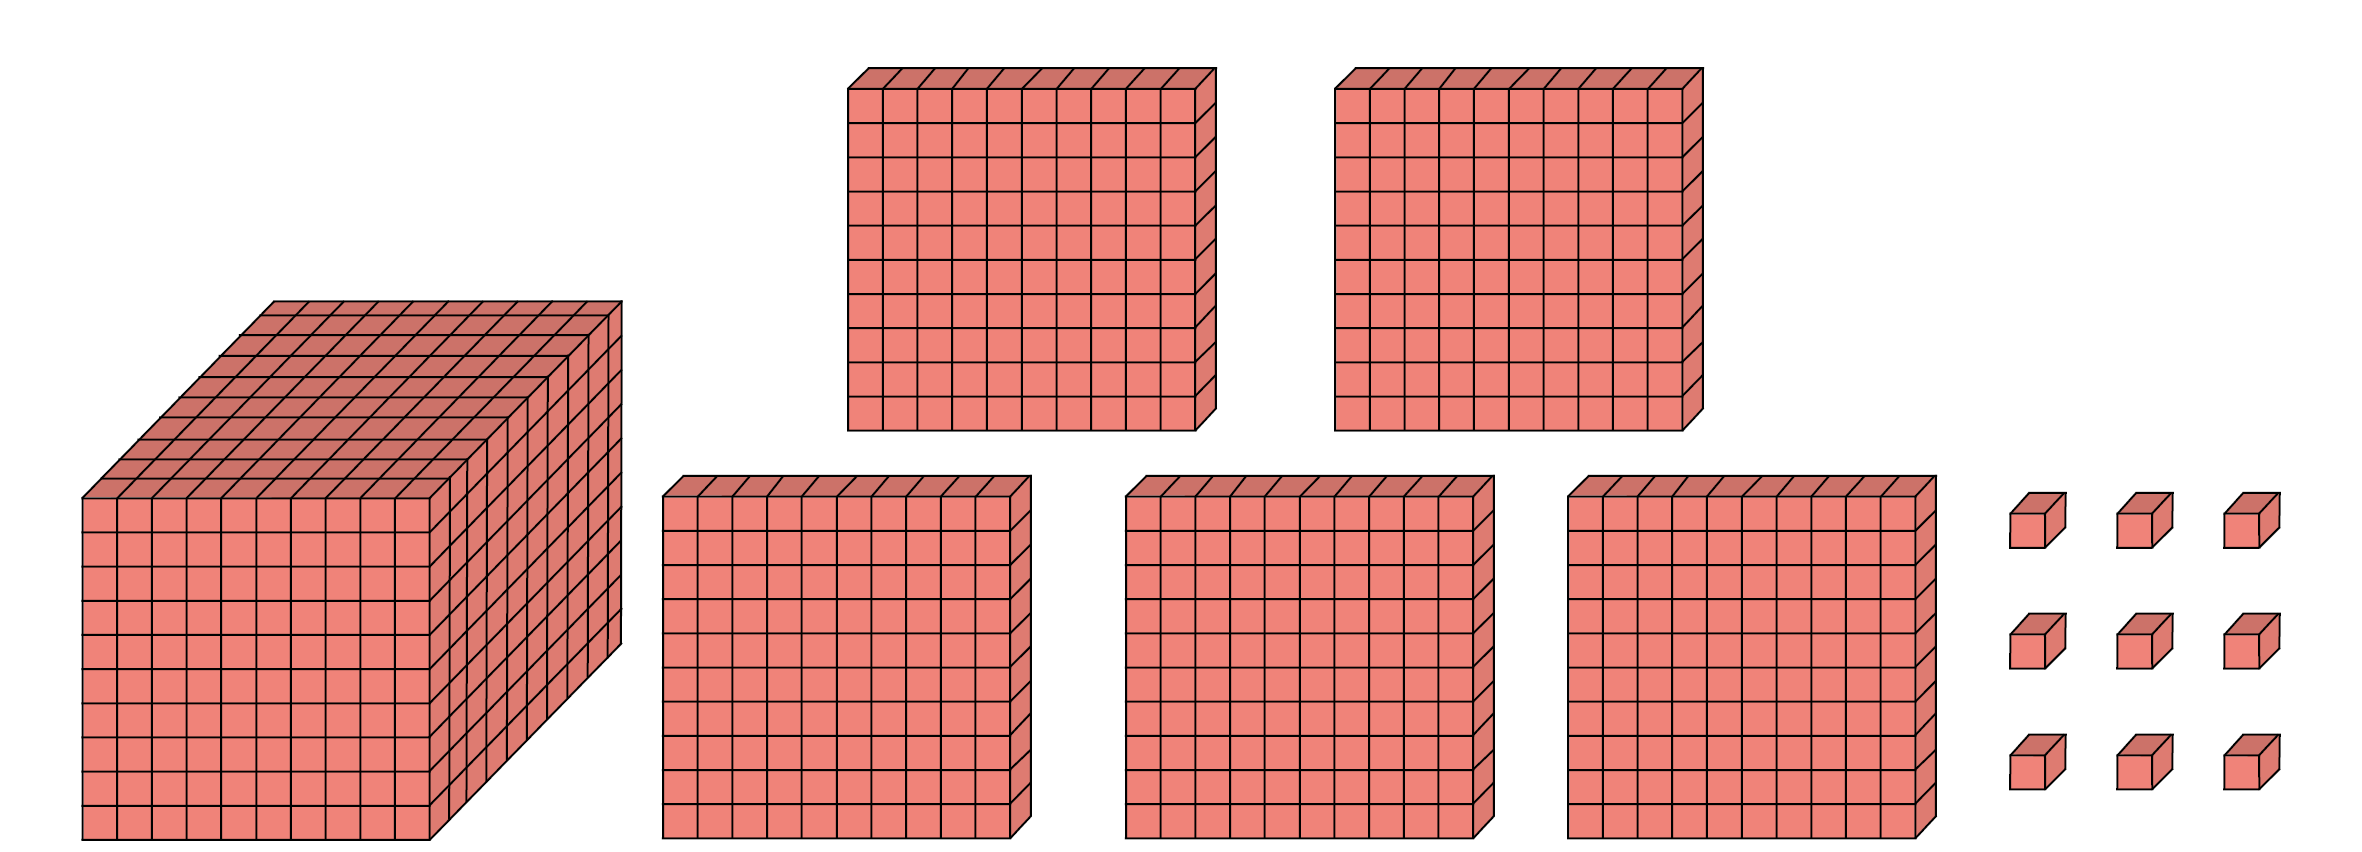
\includegraphics[width=\textwidth]{../ilustracoes/MAT5/SAEB_5ANO_MAT_figura4.png}
\end{figure}

Qual o número representado por Ana Letícia?

\coment{ 1.509
1 x 1.000 + 5 x 100 + 1 x 9 = 1.509.}

\num{6} Leia o diálogo que ocorreu entre um vendedor de carros e a pessoa interessada em comprar o carro.

\begin{figure}[htpb!]
\includegraphics[width=\textwidth]{../ilustracoes/MAT5/SAEB_5ANO_MAT_figura5.png}
\end{figure}

Escreva com algarismos, em reais, o valor pelo qual o vendedor pretende vender o carro ao interessado.

\reduline{93.990 reais ou R\$93.990,00.\hfill}

\coment{Professor, explore outros exemplos com os alunos
para que realmente entendam como escrever os números utilizando algarismos.}

\num{7} Realize a correspondência entre os retângulos da coluna 1 e os
círculos da segunda coluna, traçando linhas retas.

\begin{multicols}{2}
\blue{O maior número com exatamente 4 ordens.}

\blue{O segundo maior número formado por 4 ordens.}

\blue{Um número ímpar com 6 ordens.}

\blue{Um número de 6 ordens com algarismo da unidade de milhar igual a 3}

\red{143.254}

\red{644.821}

\red{9.999}

\red{9.998}
\end{multicols}

\coment{
“O maior número com exatamente 4 ordens” deverá estar ligado a 9.999.
“O segundo maior número formado por 4 ordens” deverá estar ligado a 9.998.
“Um número ímpar com 6 ordens” deverá estar ligado a 644.821.
“Um número de 6 ordens com algarismo da unidade de milhar igual a 3” deverá estar ligado a 143.254.

Professor, explore ao máximo o conceito de par e ímpar e já comece a
introduzir o conceito sequencial dos números naturais, em que após um par
sempre vem um ímpar e em que depois de um ímpar sempre vem um par (desde que
estejam todos os números naturais escritos).

Além disso, já pode ser introduzido o conceito de sucessor e antecessor, que aparecerá mais à frente, dizendo que 9.999 é sucessor de 9.998, e que 9.998
é o antecessor de 9.999.}

\num{8} Felipe quer realizar uma corrida e resolveu planejá-la. Para isso,
fez uma linha reta e nela marcou intervalos de 1 km, como na representação a seguir.

\begin{figure}[htpb!]
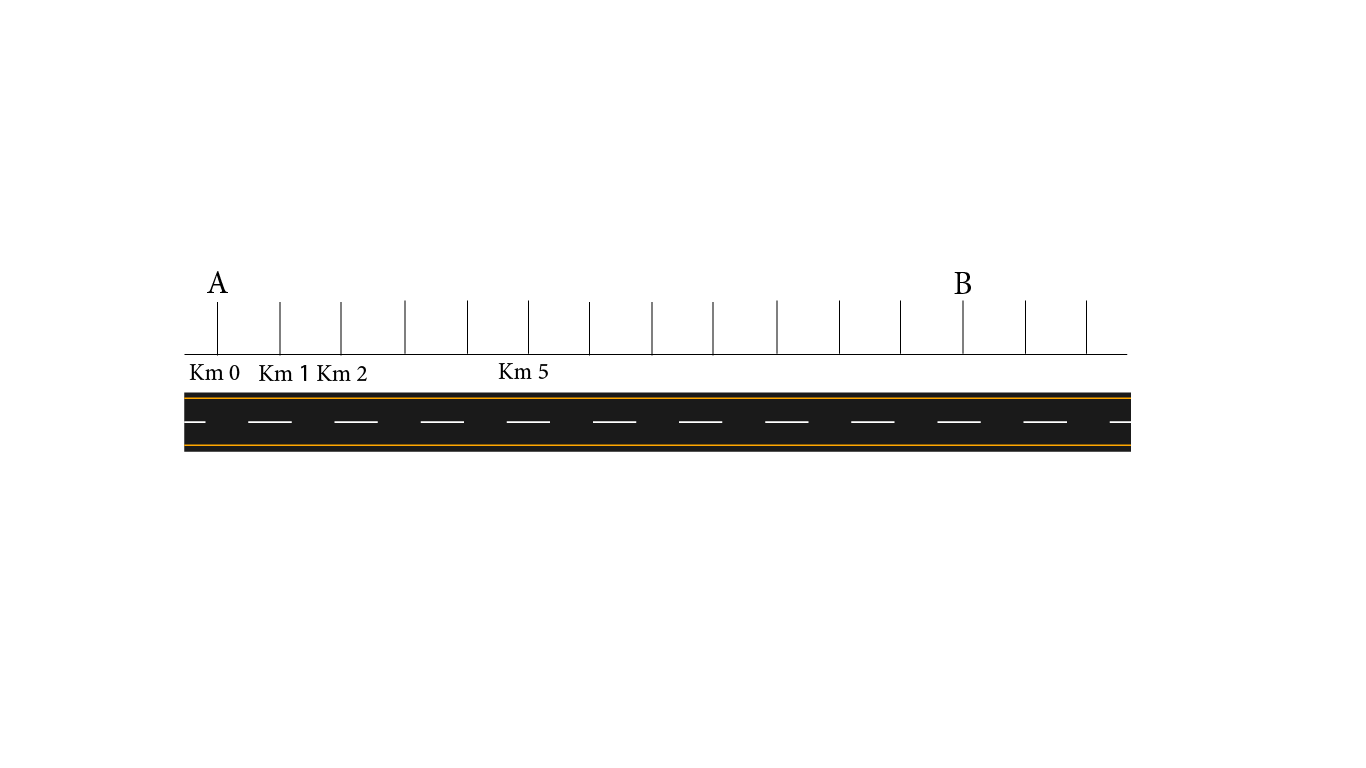
\includegraphics[width=\textwidth]{../ilustracoes/MAT5/SAEB_5ANO_MAT_figura6.png}
\end{figure}

Ele pretende começar no ponto A e terminar no ponto B. Se Felipe
conseguir completar a corrida, ele terá parado na marcação:

\begin{escolha}
\item
  Km 9
\item
  Km 10
\item
  Km 11
\item
  Km 12
\end{escolha}

\coment{
Como ele saiu do ponto A, que está em cima da marcação km 0, e chegou ao
ponto B, que está a 12 marcações de distância do ponto, podemos concluir
que ele parou no km 12, ou seja, percorreu 12 km.

Explore ao máximo com os alunos a colocação dos números na reta numérica,
já que é um conceito essencial para outros tópicos do conteúdo.}

\num{9} Complete a frase com o número que representa quanto mede cada um
dos objetos indicados a seguir.

\begin{escolha}
\item O lápis a seguir mede \reduline{11 cm}

\begin{figure}[htpb!]
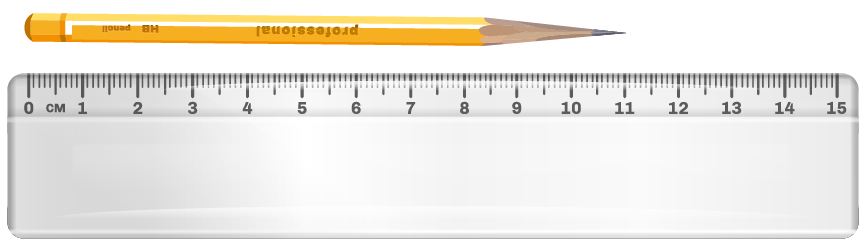
\includegraphics[width=\textwidth]{../ilustracoes/MAT5/SAEB_5ANO_MAT_figura7.png}
\end{figure}

\item A borracha representada mede \reduline{5 cm}

\begin{figure}[htpb!]
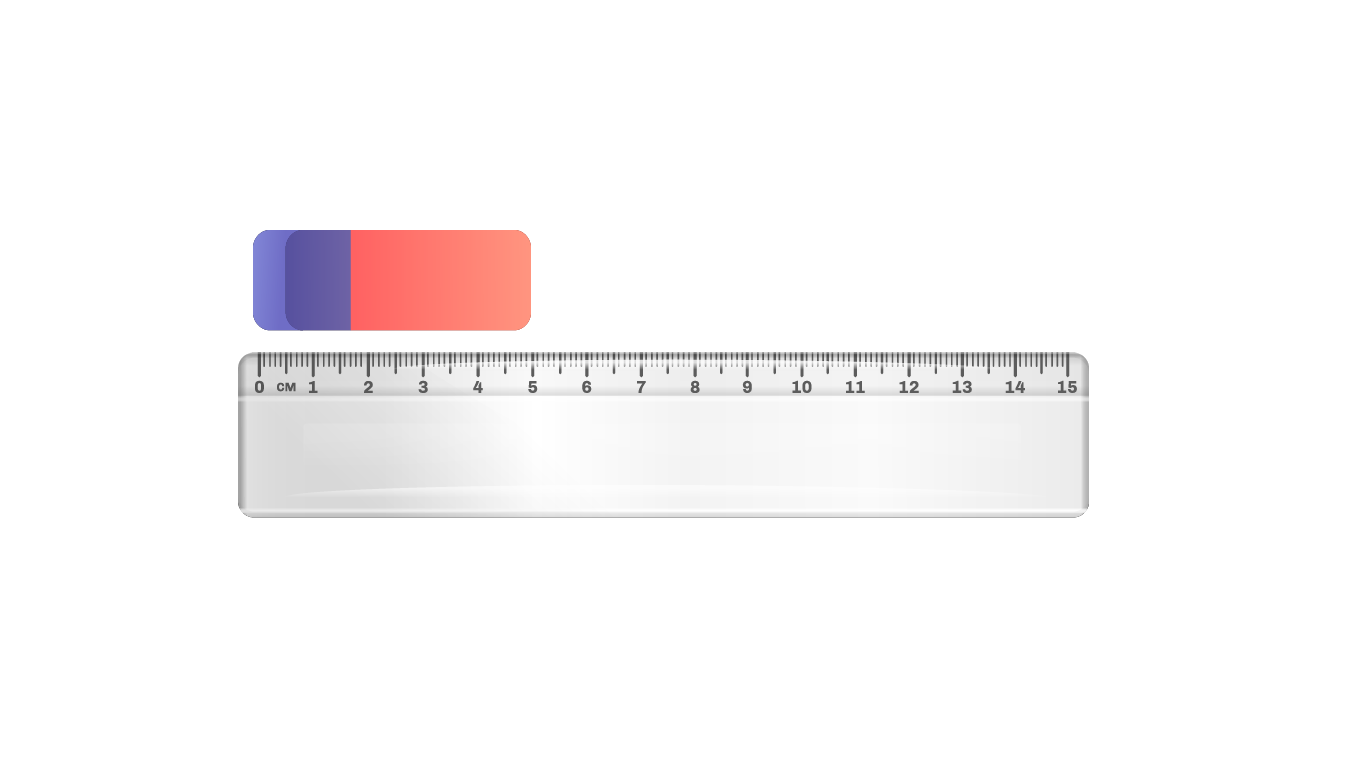
\includegraphics[width=\textwidth]{../ilustracoes/MAT5/SAEB_5ANO_MAT_figura8.png}
\end{figure}

\item O apontador da imagem mede \reduline{3 cm}

\begin{figure}[htpb!]
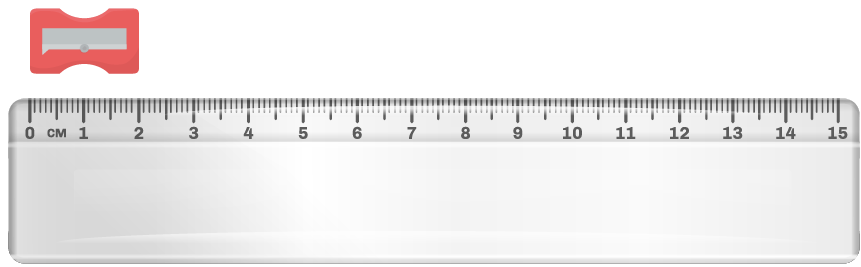
\includegraphics[width=\textwidth]{../ilustracoes/MAT5/SAEB_5ANO_MAT_figura9.png}
\end{figure}

\item A tesoura a seguir mede \reduline{10 cm}

\begin{figure}[htpb!]
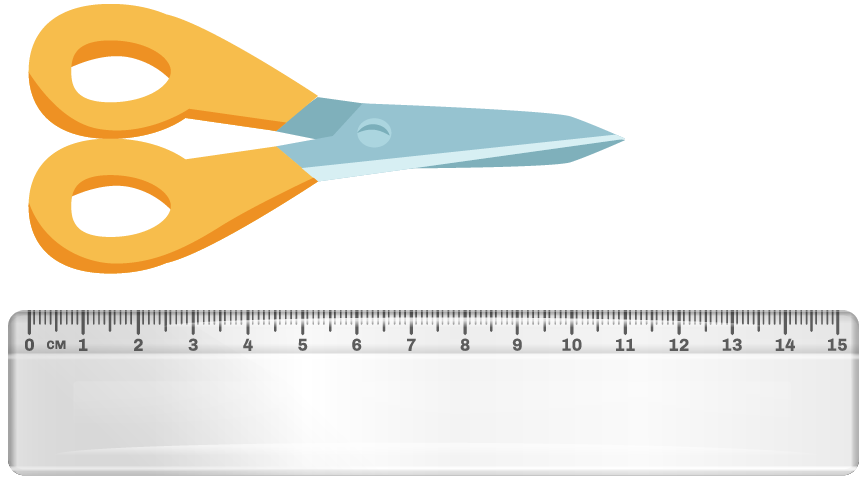
\includegraphics[width=\textwidth]{../ilustracoes/MAT5/SAEB_5ANO_MAT_figura10.png}
\end{figure}

\end{escolha}

\coment{Professor, explore bastante a habilidade de medir com o auxílio da reta
numérica, principalmente quando o início não está no zero. Esse conceito é
muito útil para entendimento de assuntos que virão em outros anos e
trabalhar bastante agora pode ser extremamente importante para o desenvolvimento do aluno em anos
posteriores.}

\num{10} A esferas representadas a seguir fazem parte de um jogo conhecido como
“bilhar” ou “sinuca”.

\begin{figure}[htpb!]
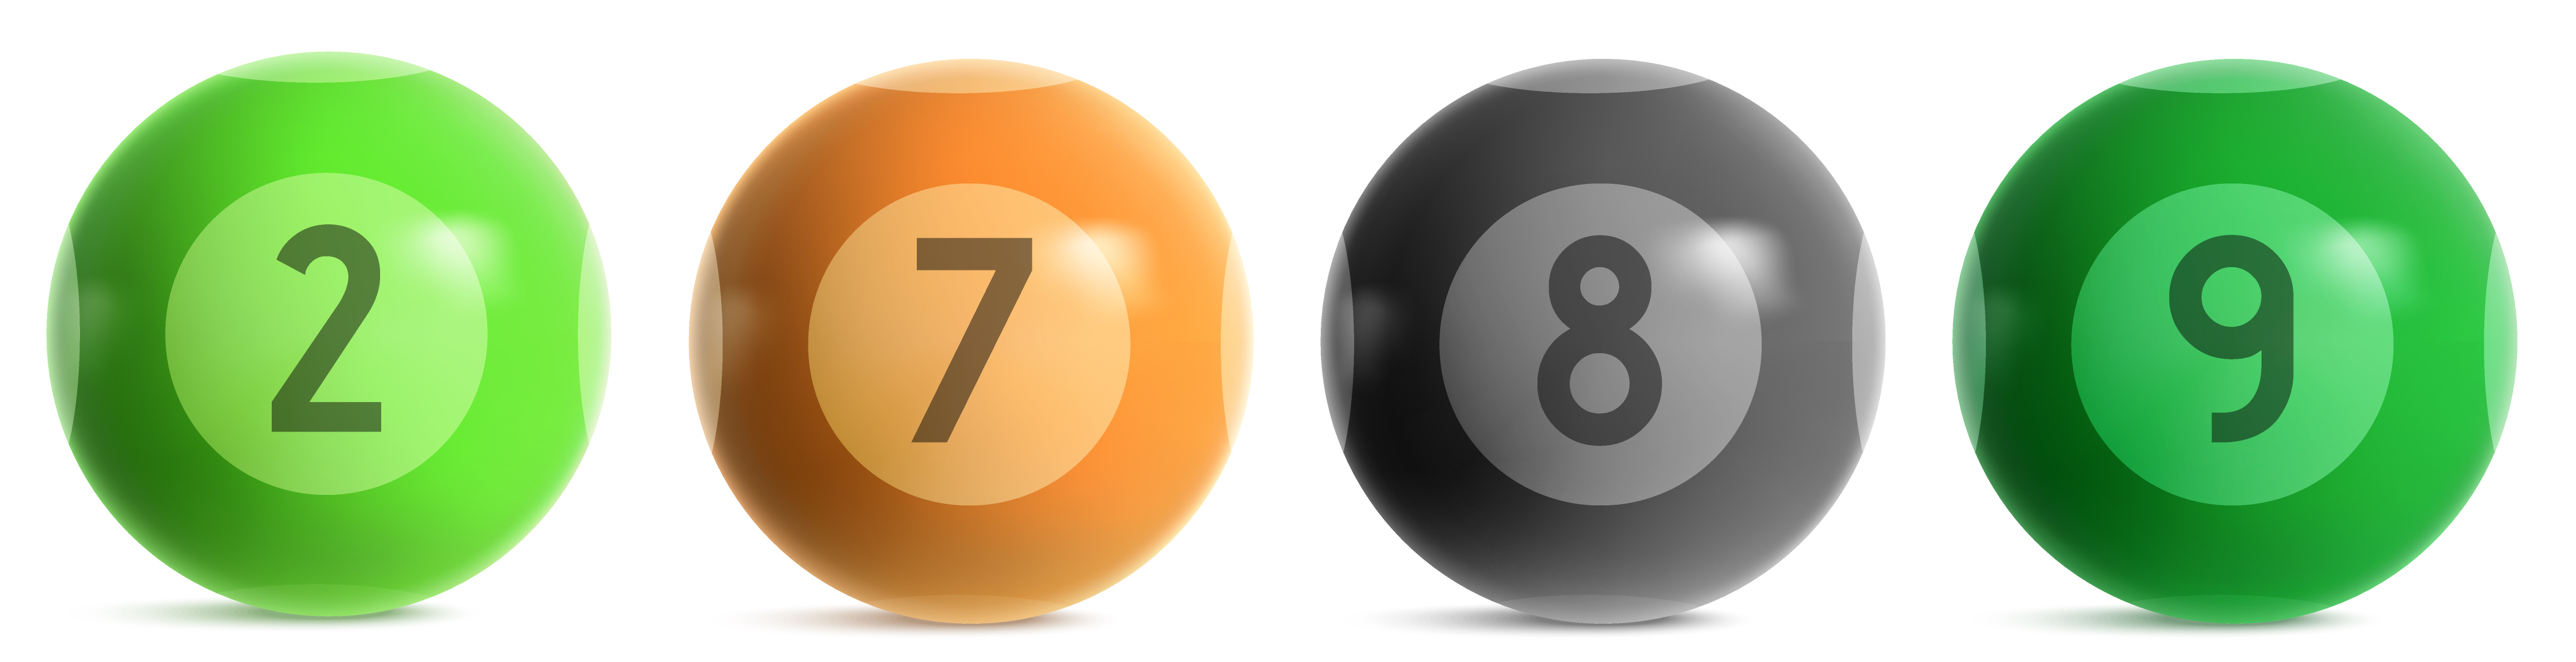
\includegraphics[width=\textwidth]{../ilustracoes/MAT5/SAEB_5ANO_MAT_figura11.png}
\end{figure}

Observando os números representados em cada esfera, responda:

\begin{escolha}
\item  Qual o maior número?

\reduline{9 (nove).\hfill}

\item  Qual o menor número, com exatamente 3 ordens, que se pode formar?

\reduline{278 (duzentos e setenta e oito).\hfill}

\item  Qual o maior número par que se pode formar?

\reduline{9.872 (nove mil oitocentos e setenta e dois).\hfill}

\end{escolha}

\coment{Explore mais exemplos com os alunos para estimular a formação de números e a criatividade de cada um deles.}

\section{Treino}


\num{1} Amanda estava brincando no escritório de seu pai quando encontrou um pedaço de papel.

\begin{figure}[htpb!]
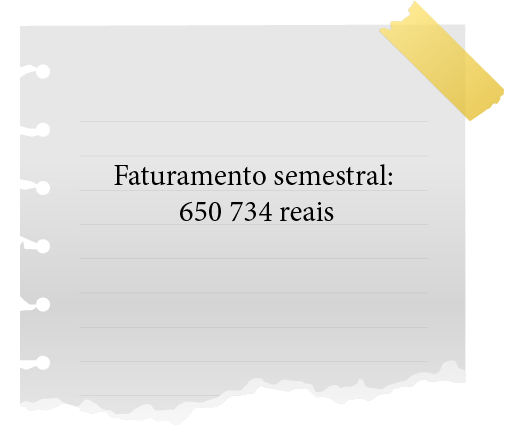
\includegraphics[width=\textwidth]{../ilustracoes/MAT5/SAEB_5ANO_MAT_figura12.png}
\end{figure}

Faturamento semestral: 650.734 reais

Lembrando das aulas de matemática, ela resolveu decompor o número escrito
no papel. Qual a decomposição correta que Amanda deverá fazer desse
número?

\begin{minipage}{.5\textwidth}
\begin{escolha}
\item
  600.000 + 50.000 + 700 + 30 + 4
\item
  600.000 + 5.000 + 70 + 3 + 4
\item
  600.000 + 500 + 700 + 30 + 4
\item
  60.000 + 50.000 + 70 + 300 + 4
\end{escolha}
\end{minipage}
\sidetext{SAEB: - Compor ou decompor números naturais de até 6 ordens na forma aditiva, ou em suas ordens, ou em adições e multiplicações.
BNCC: EF05MA01 - Ler, escrever e ordenar números naturais até a ordem das centenas de milhar com
compreensão das principais características do sistema de numeração decimal.}

\num{2} Na reta numérica a seguir, o ponto P representa o número 540 e o
ponto U representa o número 590.

\begin{figure}[htpb!]
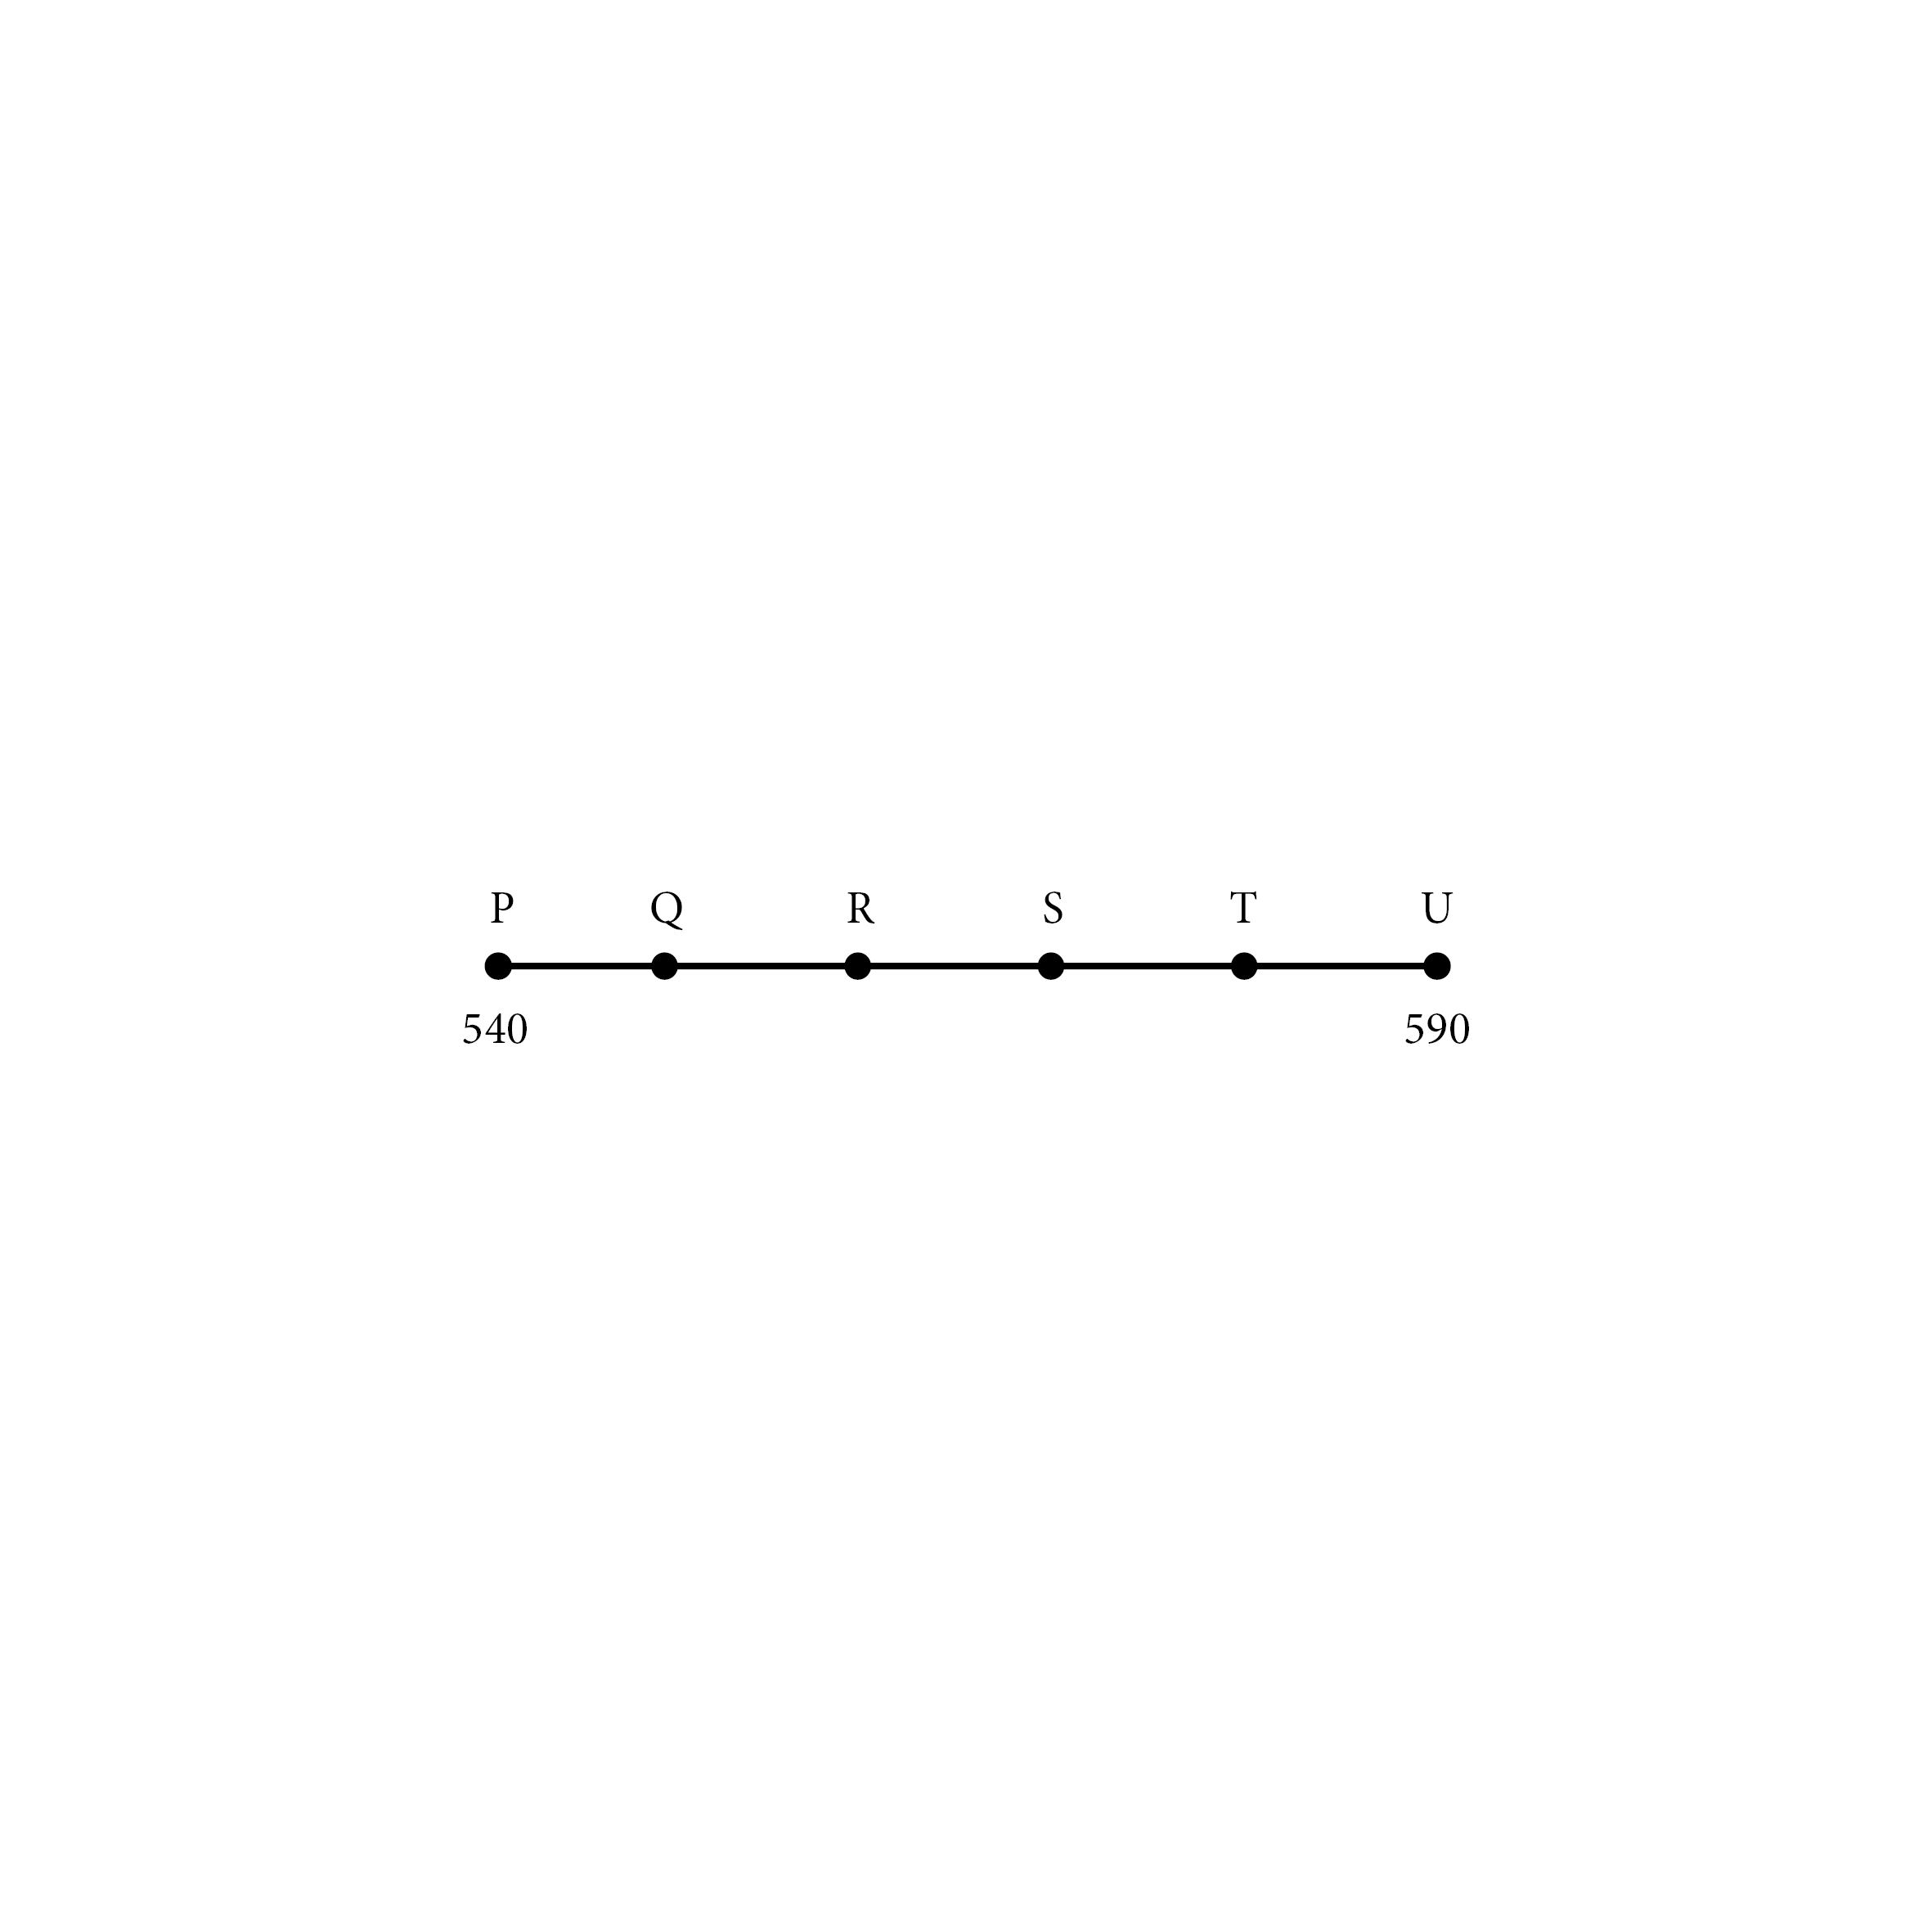
\includegraphics[width=\textwidth]{../ilustracoes/MAT5/SAEB_5ANO_MAT_figura13.png}
\end{figure}

Em qual ponto temos a representação do número 570, sabendo-se que a
distância entre dois pontos consecutivos é de 10 unidades?

\begin{minipage}{.5\textwidth}
\begin{escolha}
\item
  Q
\item
  R
\item
  S
\item
  T
\end{escolha}
\end{minipage}
\sidetext{SAEB: - Identificar a ordem ocupada por um algarismo ou seu valor posicional (ou valor relativo) em um número natural de até 6 ordens.
BNCC: EF05MA10 - Concluir, por meio de investigações, que a relação de igualdade existente
entre dois membros permanece ao adicionar, subtrair, multiplicar ou dividir cada um desses
membros por um mesmo número, para construir a noção de equivalência.}


\num{3}José resolveu comprar uma linda placa com o número de sua casa.

\begin{figure}[htpb!]
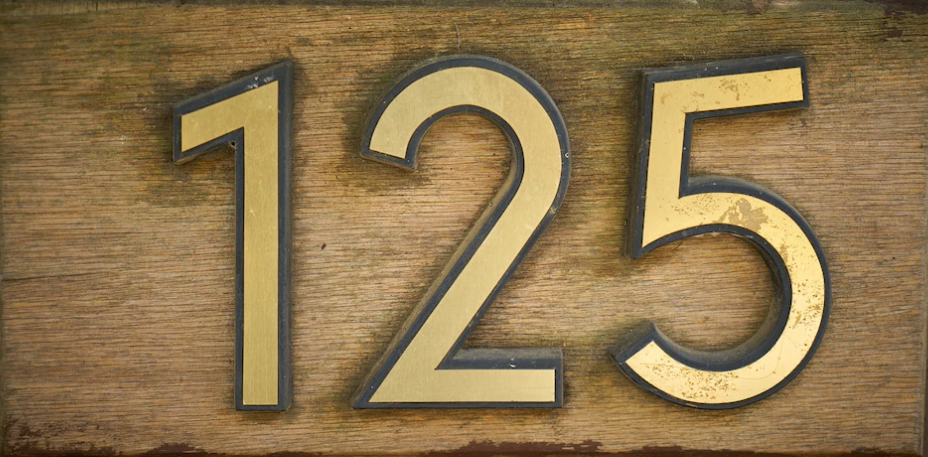
\includegraphics[width=.5\textwidth]{./imgs/mat1.png}
%https://img.freepik.com/fotos-gratis/numero-125_1122-1156.jpg?w=1060\&t=st=1677434865~exp=1677435465~hmac=526ac25f92ac28e692177f84842345ca95b5e246e04ca35259750459c4f3e954
\end{figure}

Porém, na hora de efetuar a compra, não percebeu que o número estava
errado, já que o primeiro e o último algarismos estão nas posições
trocadas. Qual é o valor relativo do último algarismo no lugar em que ele se
encontra na placa errada e qual deveria ser seu valor relativo no número
correto da casa de José?

\begin{minipage}{.5\textwidth}
\begin{escolha}
\item
  Como está: 5.\\
  Como deveria ser: 50.
\item
  Como está: 50.\\
  Como deveria ser: 500.
\item
  Como está: 5.\\
  Como deveria ser: 500.
\item
  Como está: 50.\\
  Como deveria ser: 5.
\end{escolha}
\end{minipage}
\sidetext{SAEB: - Compor ou decompor números naturais de até 6 ordens na forma aditiva, ou em suas ordens, ou em adições e multiplicações.
BNCC: EF05MA10 - Concluir, por meio de investigações, que a relação de igualdade existente
entre dois membros permanece ao adicionar, subtrair, multiplicar ou dividir cada um desses
membros por um mesmo número, para construir a noção de equivalência.}


\chapter{Multiplicar e dividir}
\markboth{Módulo 2}{}

\colorsec{Habilidades do SAEB}

\begin{itemize}
\item Calcular o resultado de adições ou subtrações envolvendo números
naturais de até 6 ordens.

\item Calcular o resultado de multiplicações ou divisões envolvendo números
naturais de até 6 ordens.

\item Associar o quociente de uma divisão com resto zero de um número
natural de até 6 ordens por 2, 3, 4, 5 e 10 às ideias de metade, terça,
quarta, quinta e décima parte.

\item Resolver problemas de adição ou de subtração, envolvendo números
naturais de até 6 ordens, com os significados de juntar, acrescentar,
separar, retirar, comparar ou completar.

\item Resolver problemas de multiplicação ou de divisão, envolvendo números
naturais de até 6ordens, com os significados de formação de grupos
iguais (incluindo repartição equitativa e medida), proporcionalidade ou
disposição retangular.
\end{itemize}

\conteudo{Professor, talvez este seja um dos módulos mais importantes, por se
tratar das quatro operações básicas. Relembre com os alunos cada detalhe delas, bem como os
algoritmos de adição, subtração, multiplicação e divisão, dando ênfase na divisão, que geralmente é o maior desafio enfrentado
pelos alunos.

Adição:

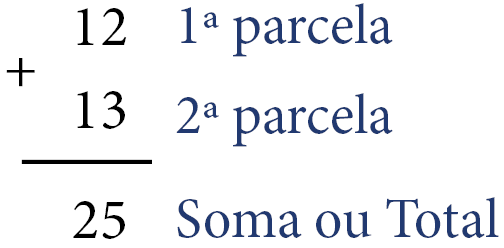
\includegraphics[width=\textwidth]{../ilustracoes/MAT5/SAEB_5ANO_MAT_figura14.png}

Subtração:

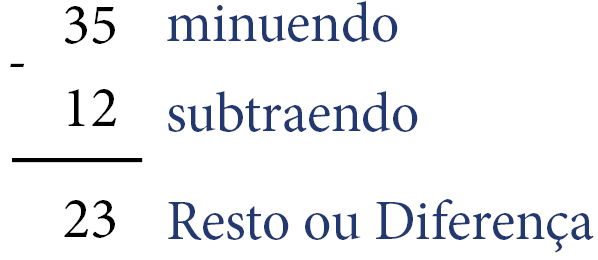
\includegraphics[width=\textwidth]{../ilustracoes/MAT5/SAEB_5ANO_MAT_figura15.png}

Multiplicação:

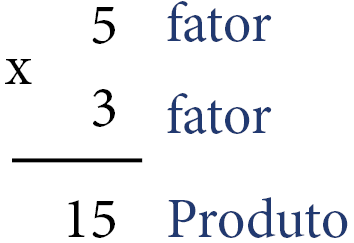
\includegraphics[width=\textwidth]{../ilustracoes/MAT5/SAEB_5ANO_MAT_figura16.png}

Divisão:

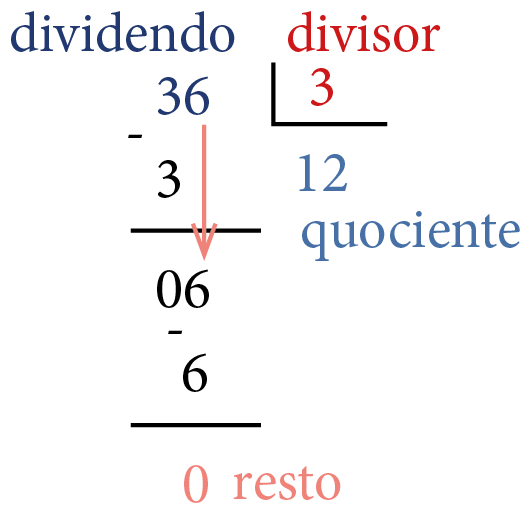
\includegraphics[width=\textwidth]{../ilustracoes/MAT5/SAEB_5ANO_MAT_figura17.png}
}

\colorsec{Atividades}

\num{1} Ligue cada operação que está na coluna 1 com o seu resultado correto na coluna 2.

\begin{multicols}{2}
584 -- 249 

960 -- 723 

767 -- 158 

50 -- 2 x (5 + 15) + 2 x 3 -- 2 x 2) + 3 x (10 -- 4 x 2) 

2 + 8 x 2 -- 2(1 + 2 x 3) 

50 -- {[}24 + 3 x (2 + 3 x 2{]} 

2 x 3 -- {[}10 -- 2 x (1 + 1 x 3){]} 

\columnbreak


237

609

335

4

6

18

2
\end{multicols}

\matlinhas{10}

\coment{
Professor, explore ao máximo com os alunos o conceito de quais operações
devem ser realizadas primeiro para, assim, fixar o conceito da ordem das operações.

584 -- 249 = 335

960 -- 723 = 237

767 -- 158 = 609

50 -- 2 x (5 + 15) + 2 x (3 -- 2 x 1) + 3 x (10 -- 4 x 2) = 50 -- 40 + 2
+ 6 = 18

2 + 8 x 2 -- 2(1 + 2 x 3) = 2 + 16 -- 14 = 4

50 -- {[}24 + 3 x (2 + 3 x 2{]} = 50 -- 48 = 2

2 x 4 -- {[}10 -- 2 x (1 + 1 x 3){]} = 8 -- 2 = 6}

\begin{figure}[htpb!]
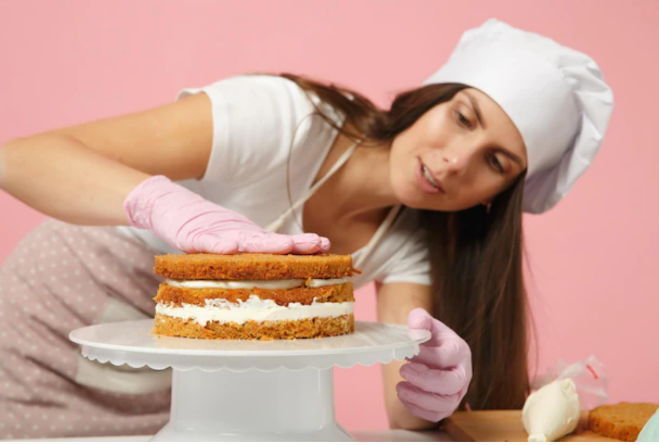
\includegraphics[width=.5\textwidth]{./imgs/mat2.png}
%https://img.freepik.com/fotos-premium/chef-cozinheiro-confeiteiro-ou-padeiro-em-t-shirt-branca-toque-chefs-chapeu-cozinhando-na-mesa-isolada-em-fundo-rosa-pastel-em-estudio-aplicacao-de-creme-processo-de-confeccao-de-bolos-mock-up-conceito-de-comida-de-espaco-de-copia_365776-27137.jpg?w=1060
\end{figure}

\num{2} A receita de um bolo diz que inicialmente devemos colocar 260 g de
farinha de trigo e misturar com outros ingredientes como ovos, açúcar e
leite. Um seguida, devemos colocar mais 135 g de farinha de trigo para a
massa ficar no ponto ideal. Qual foi a quantidade total de farinha
utilizada nessa receita?


\matlinhas{3}

\coment{260 + 135 = 395 g.}

\num{3} O estado de São Paulo tem muitas cidades, sendo que muitas delas com
centenas de milhares de habitantes. A tabela mostra a população estimada
de algumas cidades paulistas.

\begin{longtable}[]{@{}ll@{}}
\toprule
Município & População estimada\tabularnewline
\midrule
\endhead
São Paulo & 12.396.372\tabularnewline
Campinas & 1.223.237\tabularnewline
Ribeirão Preto & 720.116\tabularnewline
Franca & 358.539\tabularnewline
São Carlos & 256.915\tabularnewline
\bottomrule
\end{longtable}

\fonte{Dados IBGE.}

Sem considerar a cidade de São Paulo, a soma da população estimada das
outras quatro cidades é maior ou menor do que a quantidade de habitantes
da cidade de São Paulo? Justifique com cálculos.

\matlinhas{5}

\coment{1.223.237 + 720.116 + 358.539 + 256.915 = 2.558.807.

Portanto, a soma das populações estimadas dos municípios apresentados na
tabela, exceto São Paulo, é menor que a população da cidade de São Paulo.}

\num{4} Raquel sempre gostou muito de cozinhar e,
querendo muito trabalhar com isso, ela decidiu começar uma pequena
empresa que faz doces para festas. Para o próximo final de semana, recebeu a seguinte encomenda por mensagem de texto em seu celular:

\begin{figure}[htpb!]
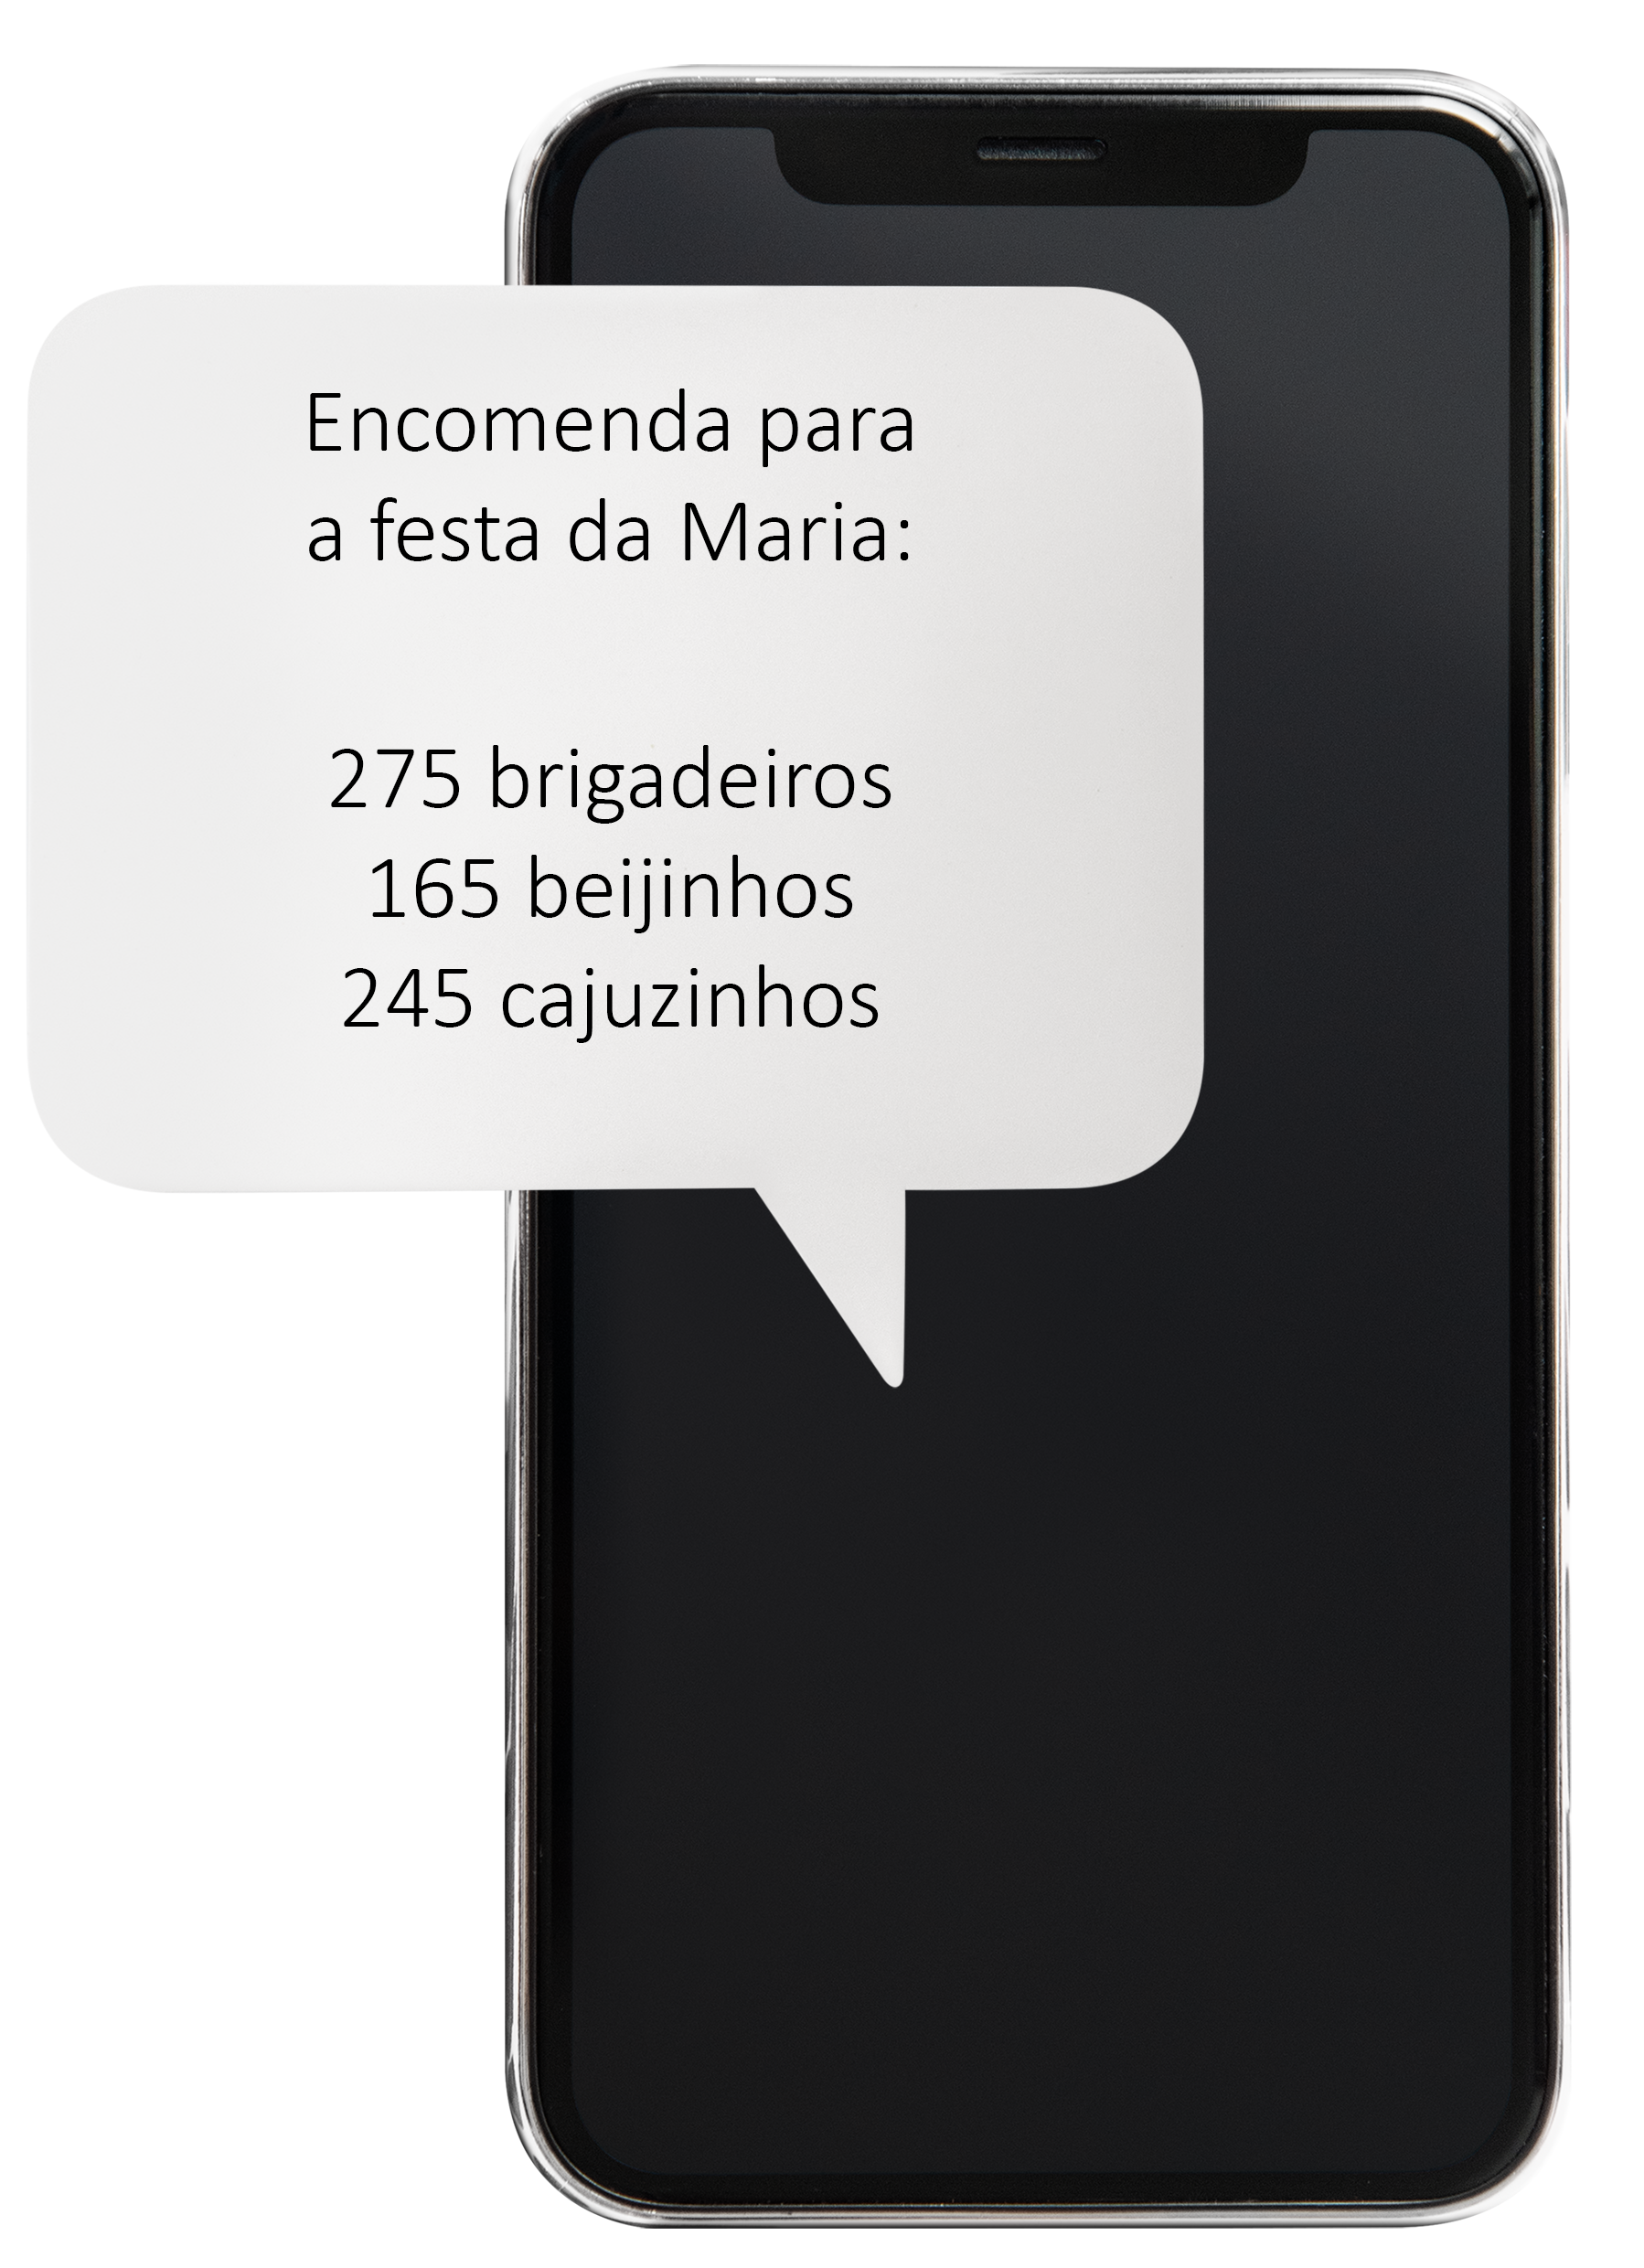
\includegraphics[width=\textwidth]{../ilustracoes/MAT5/SAEB_5ANO_MAT_figura18.png}
\end{figure}

Calcule o total de unidades de doces que Raquel terá que fazer para entregar essa encomenda completa.

\matlinhas{4}

\coment{275 + 165 + 245 = 685 unidades de doces.}

\num{5} Veja a pilha de caixas que Juliano guarda na garagem de sua casa.

\begin{figure}[htpb!]
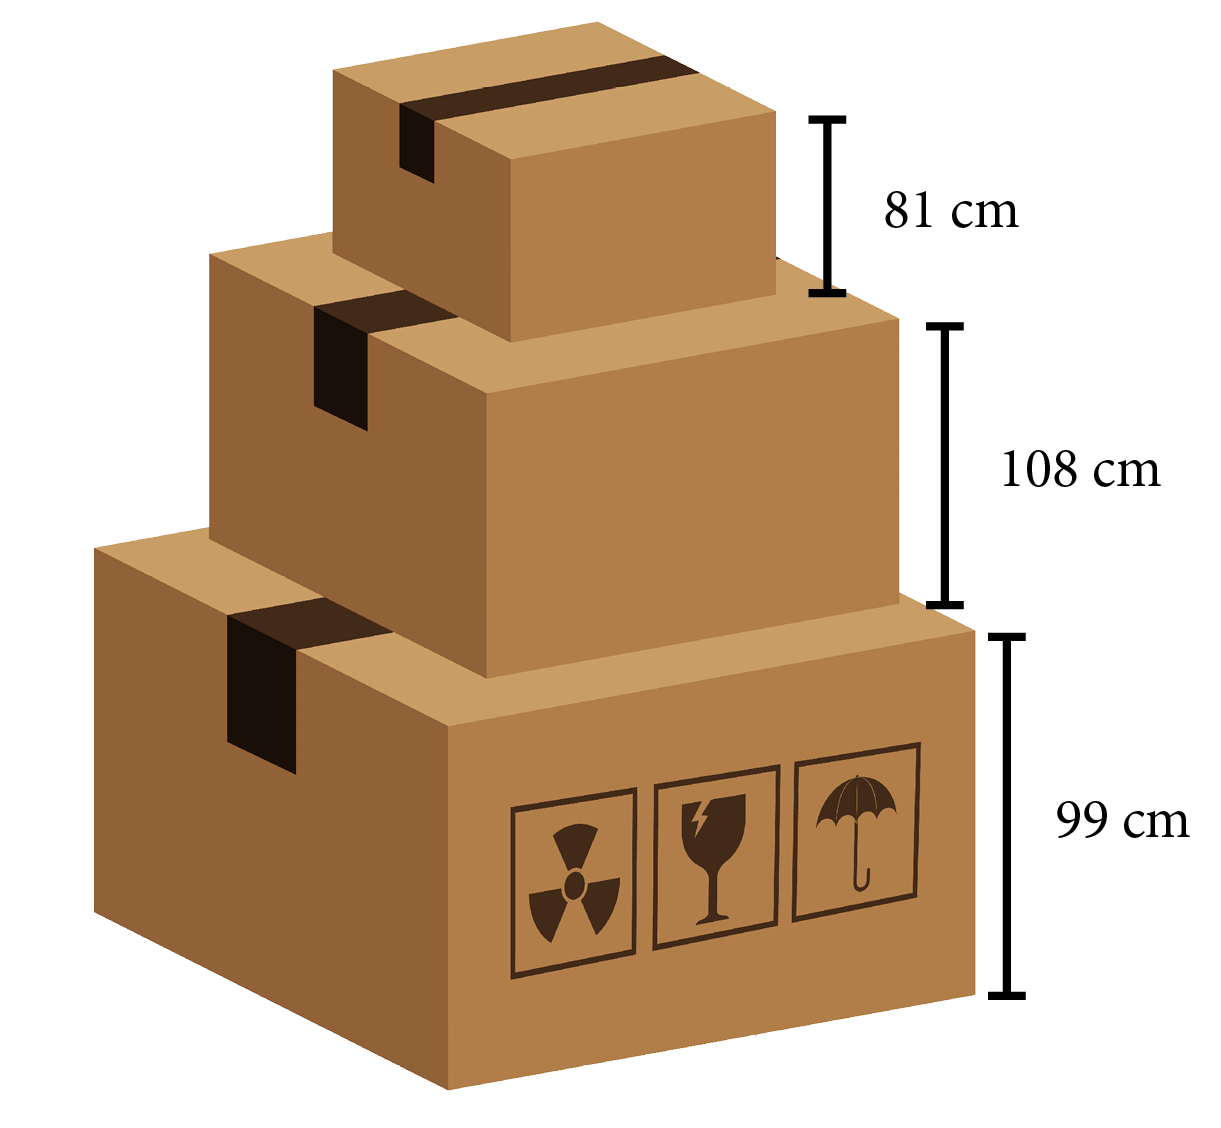
\includegraphics[width=\textwidth]{../ilustracoes/MAT5/SAEB_5ANO_MAT_figura19.png}
\end{figure}

\begin{escolha}
\item
  Qual a altura da pilha de caixas?

\matlinhas{3}

\coment{81 + 108 + 99 = 288 cm = 2,88 m}

\item
  Se Juliano inverter a ordem das caixas na hora de empilhar a altura
  total será alterada?

  \reduline{Não\hfill}
\end{escolha}

\coment{Explorar com os alunos as propriedades das operações, principalmente a
comutativa e a associativa. Deixar que os alunos troquem a ordem das caixas
no item b para perceberem que nada será alterado na soma.}

\num{6} Observe as balanças de pratos em equilíbrio representadas a seguir e, então, responda ao que se pede.

\begin{figure}[htpb!]
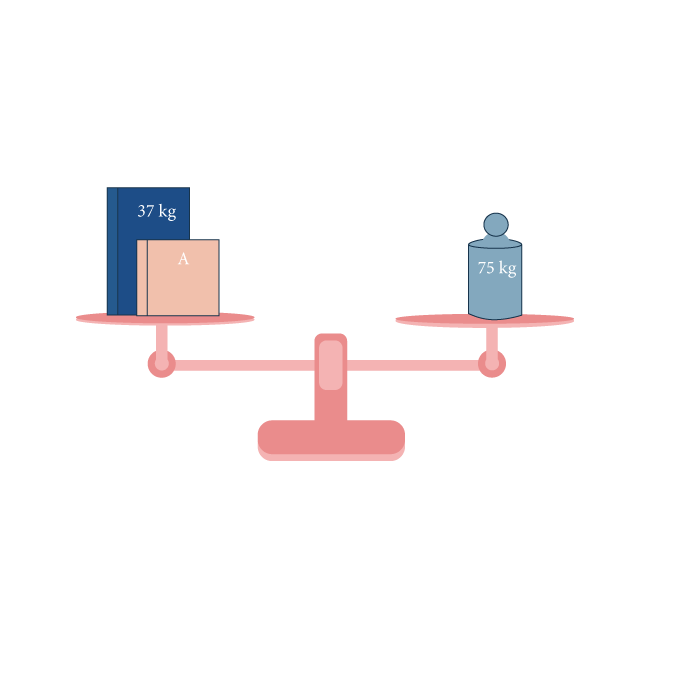
\includegraphics[width=.5\textwidth]{../ilustracoes/MAT5/SAEB_5ANO_MAT_figura20a.png}
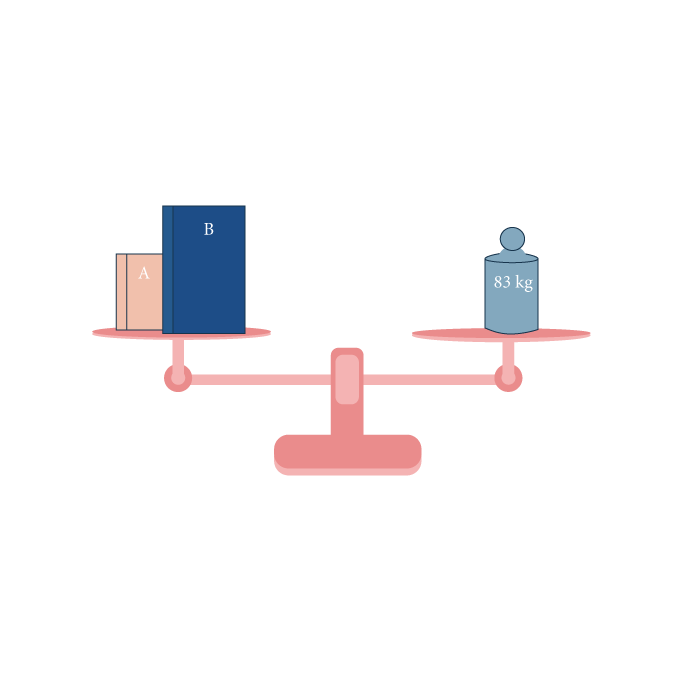
\includegraphics[width=.5\textwidth]{../ilustracoes/MAT5/SAEB_5ANO_MAT_figura20b.png}
\end{figure}

\begin{escolha}
\item Quantos quilogramas tem a caixa A?

\matlinhas{3}

\coment{75 -- 37 = 38 kg}

\item Sabendo a massa da caixa A, é possível encontrar a da caixa B? Se sim,
  calcule qual a massa da caixa B em quilogramas.

\matlinhas{3}

\coment{O cálculo é possível.

83 -- 37 = 46 Kg

Professor, comece a explorar o conceito de igualdade e, aos poucos, os conceitos primários de equações.}
\end{escolha}

\begin{figure}[htpb!]
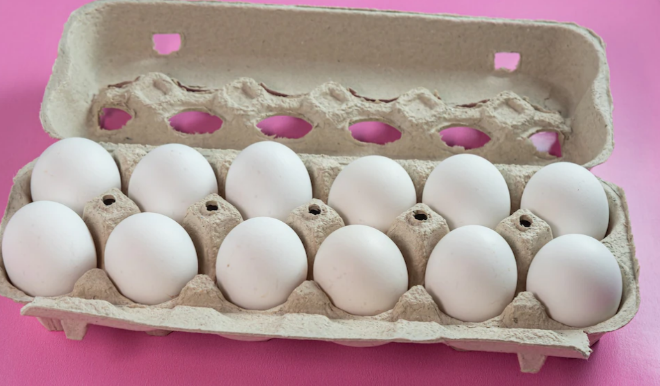
\includegraphics[width=.5\textwidth]{./imgs/mat3.png}
%https://img.freepik.com/fotos-gratis/ovos-na-superficie-rosa_58702-1950.jpg?w=1060\&t=st=1677435684~exp=1677436284~hmac=6c6204dcded4c4d80a06169fee49d53df4b2636105a2c7b3dbe5365007ceae9a
\end{figure}

\num{7} João possui uma distribuidora de ovos e acabou de receber 14 caixas
com 300 ovos cada uma. Para que João venda essa mercadoria, ele faz
embalagens com 12 ovos cada uma. Quantas embalagens João conseguirá
fazer para colocar à venda utilizando os ovos que acabou de receber em
sua loja?


\matlinhas{3}

\coment{(14 x 300):12 = 350 embalagens com 12 ovos cada uma.

Professor, sempre escreva a expressão formada pela interpretação do
enunciado, pois, assim, os alunos compreendem com mais clareza a transformação de textos em linguagem
matemática.}

\num{8} Brenda se deparou com uma divisão em sua prova de matemática. Para
esse cálculo, tínhamos 5.654 como dividendo e 24 como divisor. Sabendo-se
que Brenda acertou essa questão, qual foi o quociente encontrado por ela?

\matlinhas{4}

\coment{5.664 : 24 = 236.

Explore também divisões com dividendos maiores.}

\num{9} O pai de Pedro propôs um grande desafio para ele. O desafio
consistia em o pai fornecer uma conta com um número escondido e o filho descobrir qual seria esse número secreto. Ajude Pedro com esse
desafio e encontre o número que está escondido pelo quadrado.

\begin{figure}[htpb!]
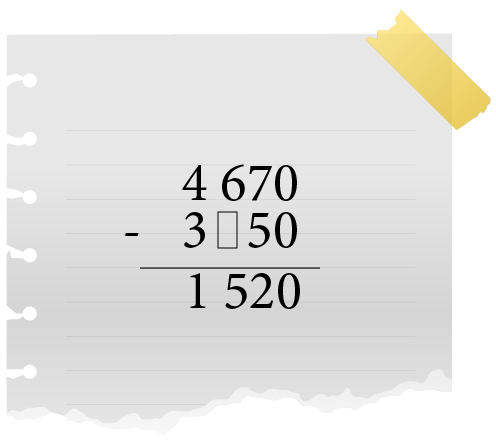
\includegraphics[width=\textwidth]{../ilustracoes/MAT5/SAEB_5ANO_MAT_figura21.png}
\end{figure}

\coment{Realizando a conta de subtração, percebe-se facilmente que o número escondido pelo quadrado é o algarismo 1.}

\num{10} A mãe de Beatriz comprou uma caixa de bombons para presentear seus
quatro filhos. Na caixa os bombons estavam distribuídos em 3 fileiras
com 12 bombons em cada. Se ela irá dividir a quantidade total de bombons
igualmente entre seus filhos, quantos bombons Beatriz receberá?

\matlinhas{3}

\coment{(3 x 12) : 4 = 9 bombons para cada um de seus filhos.}

\colorsec{Treino}

\num{1} Verificando algumas atividades realizadas na escola no ano anterior
Gustavo se deparou com a seguinte conta em que um dos números estava
coberto por um retângulo.

\begin{figure}[htpb!]
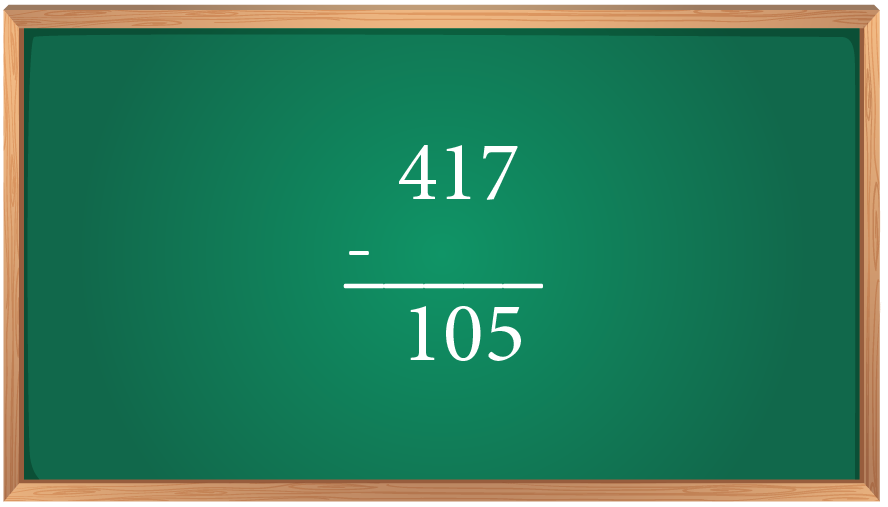
\includegraphics[width=\textwidth]{../ilustracoes/MAT5/SAEB_5ANO_MAT_figura22.png}
\end{figure}

Gustavo ficou curioso e resolveu refazer a atividade para descobrir o
número que faltava e, após alguns minutos, conseguiu descobrir. Qual o número que Gabriel encontrou?

\begin{minipage}{.5\textwidth}
\begin{escolha}
\item
  128
\item
  312
\item
  158
\item
  256
\end{escolha}
\end{minipage}
\sidetext{SAEB: Calcular o resultado de adições ou subtrações envolvendo números naturais de até 6 ordens.
Não há correspondência com a BNCC do quinto ano.}

\num{2} Isac estava conferindo o estoque de mercadorias de sua loja e
percebeu que, inicialmente, ele tinha 200 peças; depois, vendeu 2 caixas com peças para Carlos.

Em cada uma das caixas vendidas, havia um pacote com 5 unidades de peças e dois
pacotes com 7 peças.

Para saber a quantidade de peças que restavam no estoque Isac fez a
seguinte anotação:

\begin{quote}
200 -- 2 x (1 x 5 + 2 x 7)
\end{quote}

O resultado dessa expressão era exatamente igual à quantidade de peças
que restavam em seu estoque após a venda para Carlos. Qual é a
quantidade de peças que Isac tem agora em seu estoque?

\begin{minipage}{.5\textwidth}
\begin{escolha}
\item
  72
\item
  94
\item
  126
\item
  162
\end{escolha}
\end{minipage}
\sidetext{SAEB: Calcular o resultado de multiplicações ou divisões envolvendo números naturais de até 6 ordens.
Não há correspondência com a BNCC do quinto ano.}


\num{3} Um grande espetáculo chegou à cidade em que Rafael mora e, logo, uma fila
enorme se formou com pessoas querendo assistir. Os
ingressos começaram a ser vendidos e as pessoas começaram a entrar no
recinto. Em certo instante, sabia-se que 540 pessoas já tinham
entrado e que a capacidade máxima por espetáculo era de 1.200 pessoas. Como ainda temos 932 pessoas na fila, quantas pessoas não
conseguirão entrar para assistir à atração?

\begin{minipage}{.5\textwidth}
\begin{escolha}
\item
  268
\item
  272
\item
  294
\item
  1.440
\end{escolha}
\end{minipage}
\sidetext{SAEB: Resolver problemas de adição ou de subtração, envolvendo números naturais de até 6 ordens, com os significados de juntar, acrescentar, separar, retirar, comparar ou completar.
Não há correspondência com a BNCC do quinto ano.}


\chapter{Sequências}
\markboth{Módulo 3}{}

\colorsec{Habilidades do SAEB}

\begin{itemize}
\item Inferir ou descrever atributos ou propriedades comuns que os elementos
que constituem uma sequência recursiva de números naturais apresentam.

\item Inferir o padrão ou a regularidade de uma sequência de números
naturais ordenados, objetos ou figuras.

\item Inferir os elementos ausentes em uma sequência de números naturais
ordenados, objetos ou figuras.
\end{itemize}

\coment{Professor, durante este módulo, explore bastante a percepção de seus
alunos, deixando realmente durante a algum tempo que eles tentem
descobrir a lógica de cada sentença, possibilitando, assim, que consigam descobrir os próximos números de cada uma. Esse é um conceito essencial
para estimular a criatividade e encontrar regras “escondidas” entre os números.}

\conteudo{Uma sequência ou sucessão é um conjunto numérico ordenado, em que há sempre uma lógica de formação e continuidade.

Exemplos:

\begin{itemize}
\item
  A escalação de um time de futebol de salão em ordem alfabética:
Alan; Bruno, Fernando, Igor, Tácio.

\item
  Sequência de números naturais pares:
(0; 2; 4; 6; 8; 10; 12; ...)
\end{itemize}

Podemos ainda classificar as sequências quanto ao número de elementos:

\begin{itemize}
\item
  Finitas: Sequências que apresentam um número de termos bem definido.
  ou seja: 10 termos, 20 termos, 8 termos.
\item
  Infinitas: Sequências que apresentam infinitos números de termos como é o caso da sequência dos números naturais.
\end{itemize}

Ainda podemos classificar as sequências em:

\begin{itemize}
\item
  Crescentes: aquelas em que cada termo sucessor é maior que seu antecessor.
Exemplo: (5, 10, 15, 20, 25)

\item
  Decrescentes: aquelas em que cada termos sucessor sempre é menor do que seu antecessor.
Exemplo: (9, 7, 5, 3)
\end{itemize}
}

\colorsec{Atividades}

\num{1} Observe as sequências dadas e determine, sem fazer desenhos, a
quantidade de bolinhas que a figura 8 de cada sequência terá.

\begin{escolha}
\item\preencher\coment{25} bolinhas

\begin{figure}[htpb!]
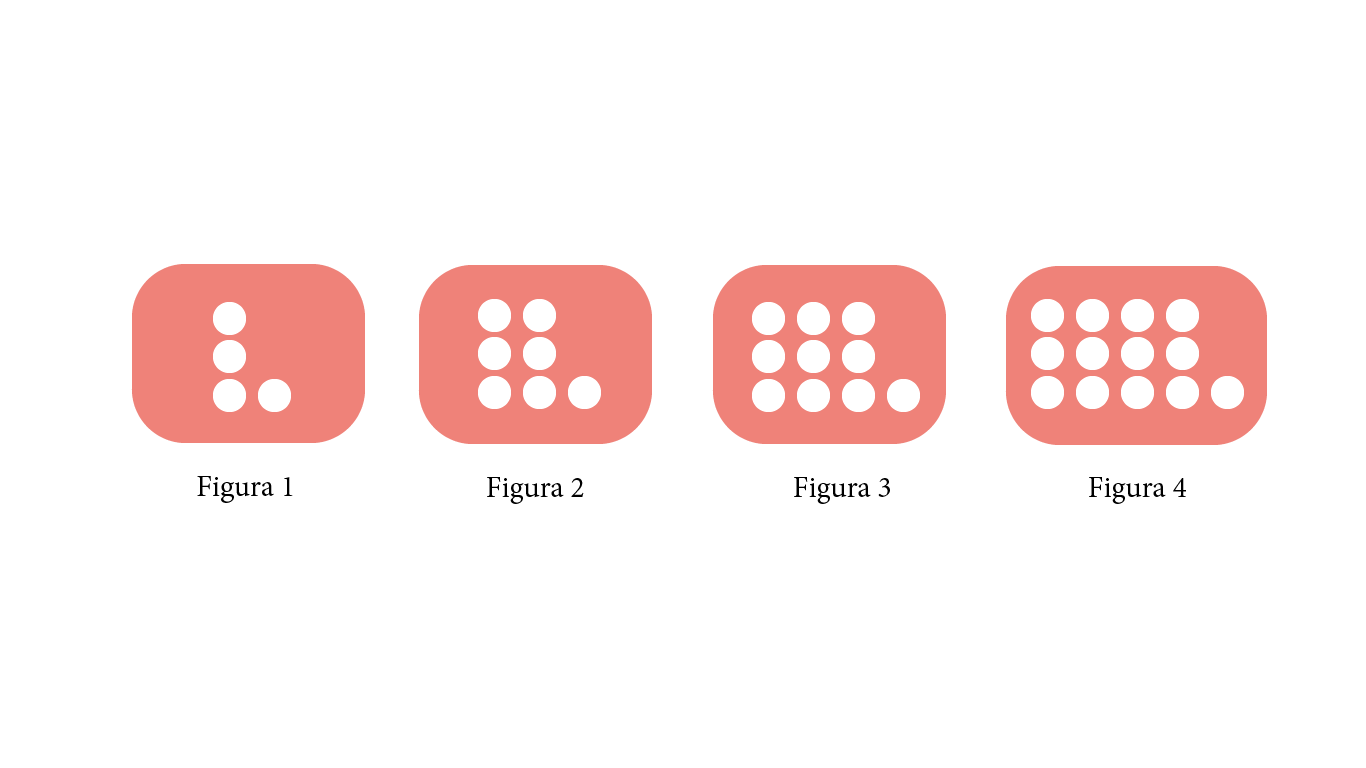
\includegraphics[width=\textwidth]{../ilustracoes/MAT5/SAEB_5ANO_MAT_figura23.png}
\end{figure}

\matlinhas{2}

\coment{(4; 7; 10; 13; 16; 19; 22; 25) ou (8 x 3) + 1 = 25}

\item\preencher\coment{24} bolinhas

\begin{figure}[htpb!]
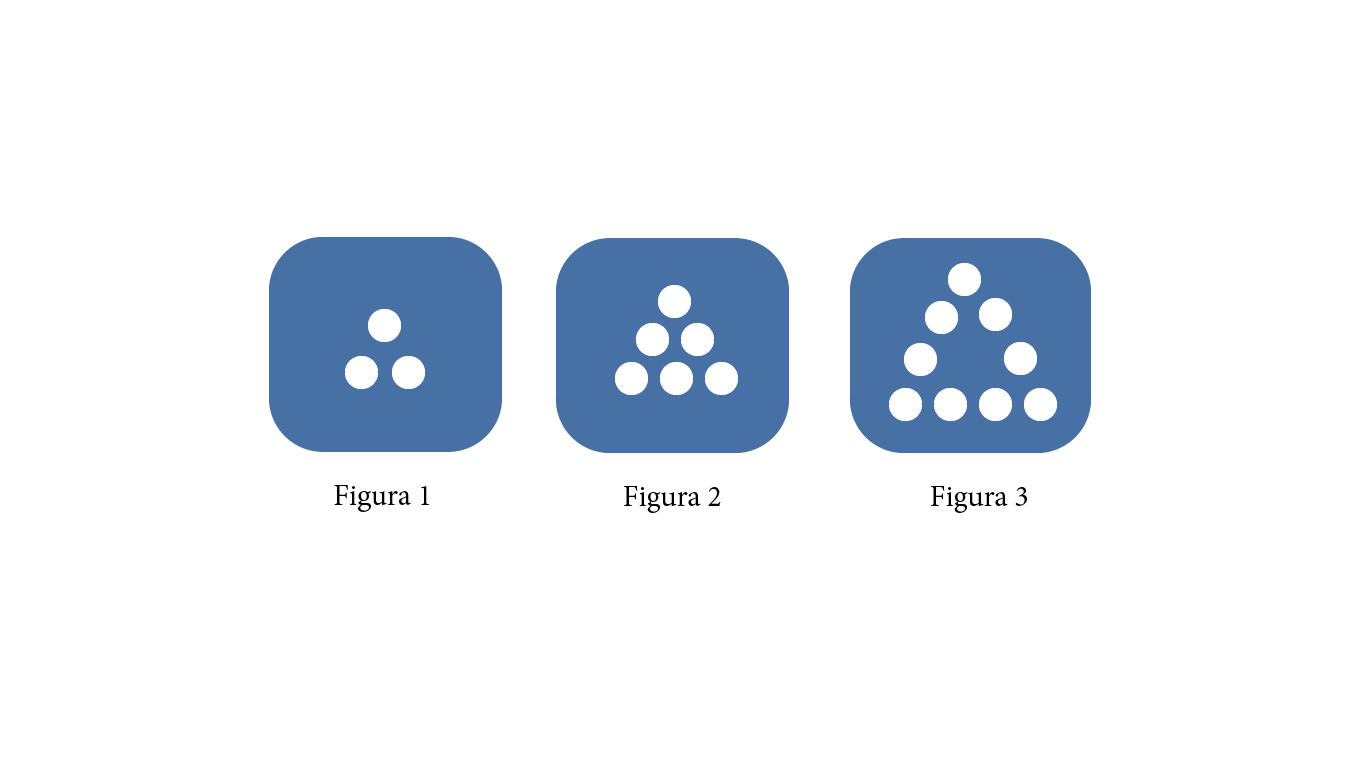
\includegraphics[width=\textwidth]{../ilustracoes/MAT5/SAEB_5ANO_MAT_figura24.png}
\end{figure}

\matlinhas{2}

\coment{(3; 6; 9; 12; 15; 18; 21; 24) ou 8 x 3 = 24}

\item\preencher\coment{32} bolinhas

\begin{figure}[htpb!]
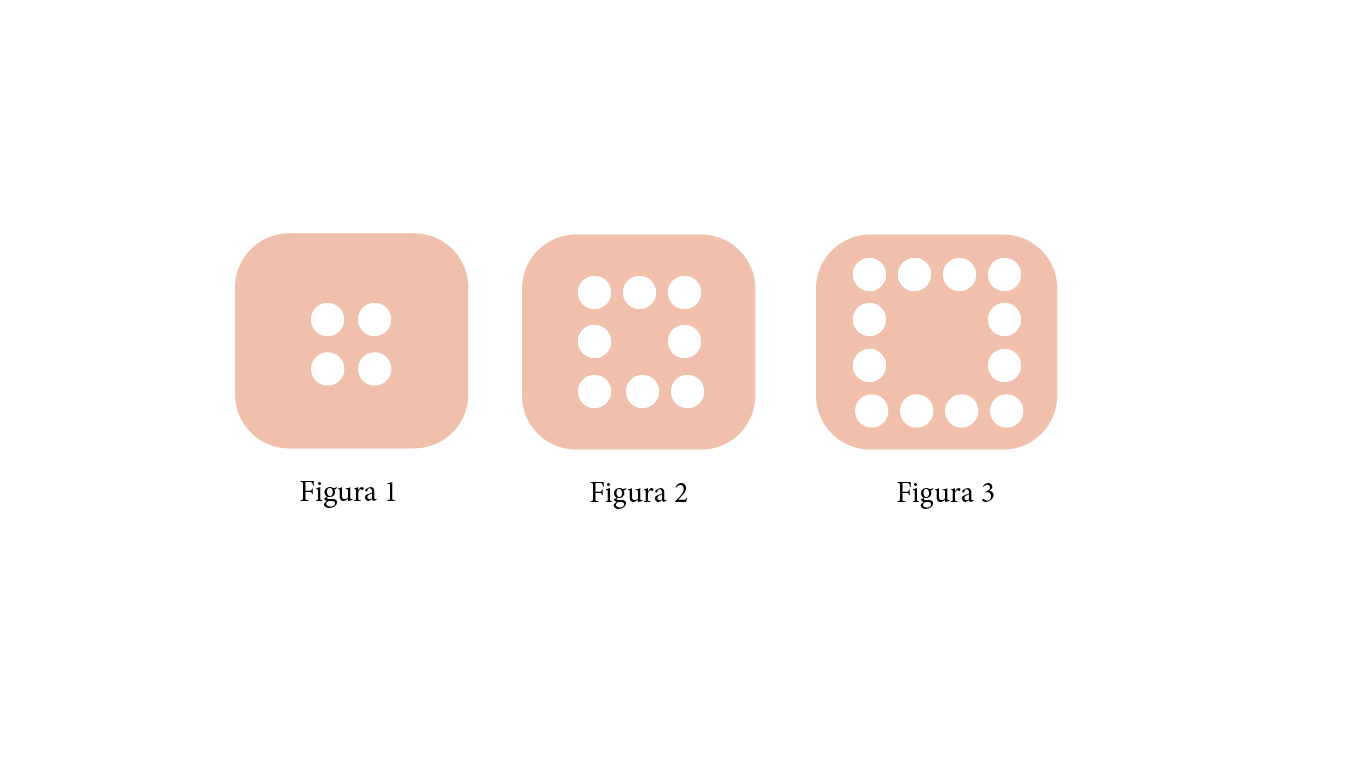
\includegraphics[width=\textwidth]{../ilustracoes/MAT5/SAEB_5ANO_MAT_figura25.png}
\end{figure}

\matlinhas{2}

\coment{(4; 8; 12; 16; 20; 24; 28; 32) ou 8 x 4 = 32}

\item\preencher\coment{40} bolinhas

\begin{figure}[htpb!]
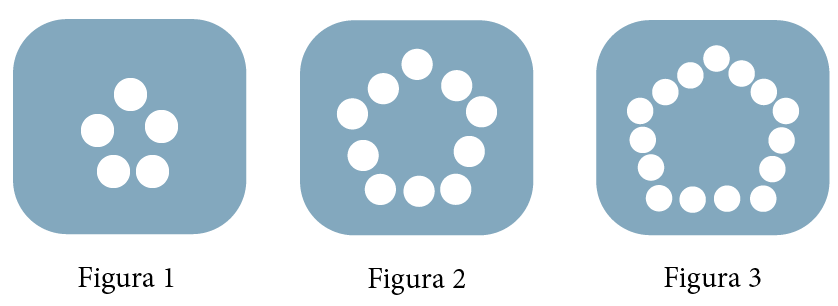
\includegraphics[width=\textwidth]{../ilustracoes/MAT5/SAEB_5ANO_MAT_figura26.png}
\end{figure}

\matlinhas{2}

\coment{(5; 10; 15; 20; 25; 30; 35; 40) ou 8 x 5 = 40}
\end{escolha}

\num{2} Genivaldo, um adulto de 45 anos, adora participar de corridas de
rua. Em uma delas ele correu com mais 49 pessoas e utilizou uma camiseta
de identificação com o número 28.

\begin{escolha}
\item
  Qual dos números que estão no texto acima representa uma
  quantidade?

\reduline{49, pois representa a quantidade de pessoas que correrem além de Genivaldo.\hfill}

\item
  Qual dos números que estão no texto acima representa um
  código?

\reduline{28, pois é o código de identificação da camiseta de Genivaldo.\hfill}

\item
  Qual dos números que estão no texto acima representa uma
  medida?

\reduline{45, pois mede a quantidade de anos que Genivaldo tem.\hfill}

\item
  Represente os números presentes no texto na forma de uma sequência
  decrescente e diga se ela é finita ou infinita.

\reduline{(49; 45; 28), que é uma sequência finita.\hfill}
\end{escolha}

\num{3} Encontre o número pedido em cada item a seguir.

\begin{escolha}
\item
  O sucessor de 3.089: \reduline{3.090 aparece, em sequência crescente, após 3.089.\hfill}
\item
  O antecessor de 4.301: \reduline{4.300 aparece, em sequência crescente, antes de 4.301.\hfill}
\item
  O sucessor e antecessor do número 3.259: \reduline{Antecessor: 3.258. Sucessor: 3.260. São os números que, em sequência crescente, aparecem antes e depois de 3.259.\hfill}
\end{escolha}

\coment{Professor, explore bastante os conceitos de sucessor e antecessor com
seus alunos, pois isso facilitará muitos entendimentos em módulos e anos futuros.}

\num{4} Ana Clara encontrou o papel representado a seguir entre os cadernos de seu irmão mais velho.

\begin{figure}[htpb!]
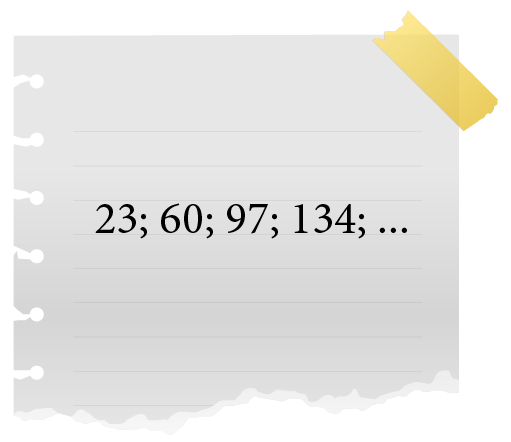
\includegraphics[width=\textwidth]{../ilustracoes/MAT5/SAEB_5ANO_MAT_figura27.png}
\end{figure}

Ela ficou muito curiosa, pois entendeu que essa era uma sequência
numérica e queria encontrar qual o próximo número dela.

Ajude Ana Clara a descobrir qual é o próximo número da sequência e o escreva no espaço que segue.

\reduline{A sequência foi montada sempre somando 37 ao número anterior para
encontrar o próximo. Portanto, o próximo número da sequência será: 134 + 37 = 171.\hfill}

\num{5} Utilizando apenas os algarismos 2, 3 e 4, escreva a sequência de
todos os números com 3 algarismos que podemos formar utilizando esses
três números sem que eles apareçam mais de uma vez em cada número.

\reduline{(234, 243, 324, 342, 423, 432)\hfill}
\linhas{2}

\num{6} O Pai de André montou a sequência de figuras a seguir.

\begin{figure}[htpb!]
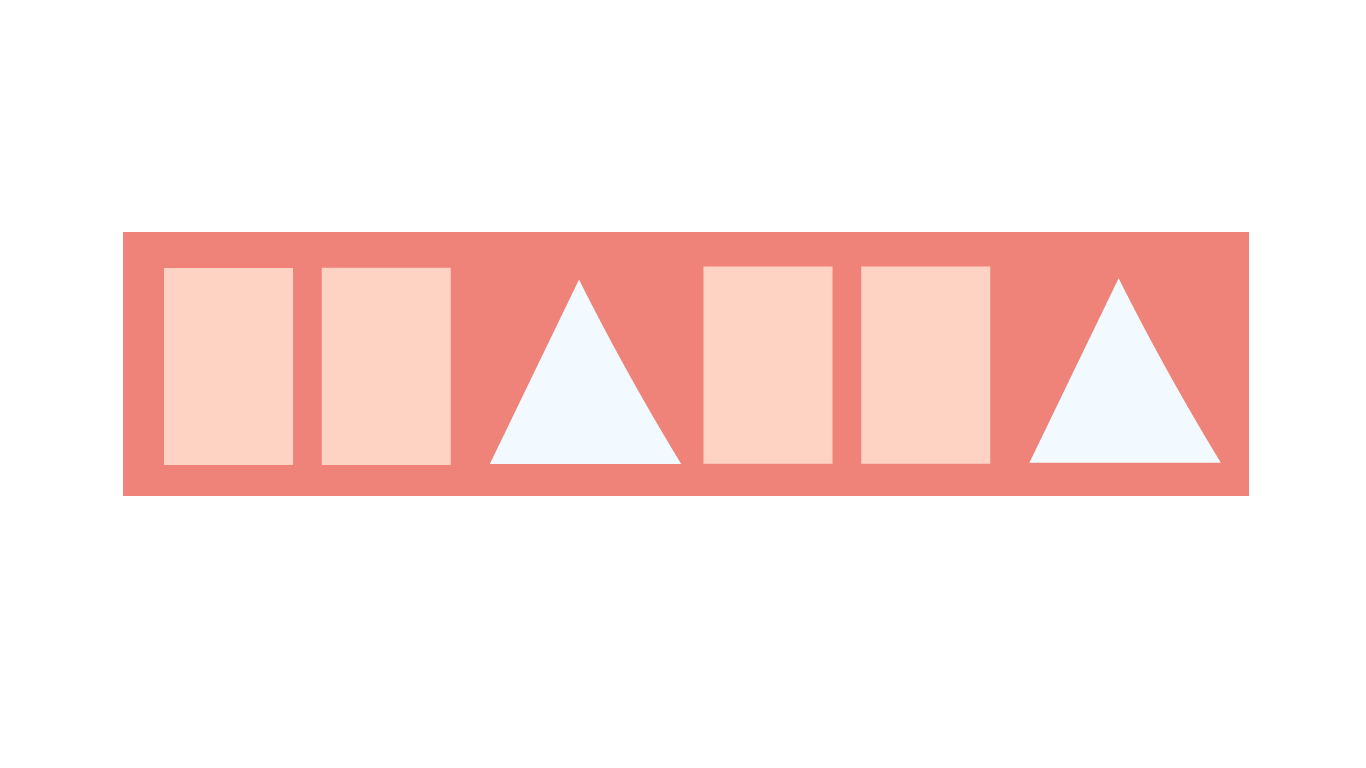
\includegraphics[width=\textwidth]{../ilustracoes/MAT5/SAEB_5ANO_MAT_figura28.png}
\end{figure}

Então, ele disse ao filho que o levaria ao cinema caso ele acertasse
qual seria o décimo termo dessa sequência. André, muito empolgado, começou a
pensar e logo deu a resposta a seu pai. O pai analisou a resposta e
disse que estava correta.

Qual a resposta que André deu a seu pai sobre qual era o décimo elemento da sequência?

\reduline{Só teremos triângulos em múltiplos de 3 e, portanto, como 10 não é um
múltiplo de 3, a figura será um quadrado. Professor, é possível que o aluno continue a sequência com desenhos até chegar à resposta. Não há problema algum e é muito válido, pois assim entenderá a lógica envolvida. \hfill}

\num{7} Relembre os conceitos de números naturais pares e ímpares e, em
seguida, resolva a atividade.

\begin{escolha}
\item
  Escreva os 10 primeiros números naturais pares em sequência crescente.
  Essa sequência é finita ou infinita? Como ela é formada?

\reduline{(0; 2; 4; 6; 8; 10; 12; 14; 16; 18). Essa é uma sequência finita e sempre
somamos 2 ao termo anterior para encontrar o próximo.\hfill}

\item
  Escreva os 12 primeiros números naturais ímpares em sequência
  crescente. Essa sequência e finita ou infinita? Como ela é formada?

\reduline{(1; 3; 5; 7; 9; 11; 13; 15; 17; 19; 21; 23). Essa é uma sequência finita
e sempre somamos 2 ao termo anterior para encontrar o próximo.
Professor, explorar como os alunos o conceito de que, na sequência dos
números naturais, após um número par sempre vem um numero ímpar; ou seja, eles se intercalam.\hfill}
\end{escolha}

\num{8} Estudando com a sua filha para a prova de matemática da semana
seguinte, Laura propõe a Luísa o seguinte exercício:

Escreva uma sequência de 6 números que aumentam de 2 em 2 unidades,
começando pelo número nove mil e novecentos e noventa e nove.

Ajude Luísa a resolver esse exercício, escrevendo os seis números pedidos no espaço demarcado.

\reduline{(9.999; 10.001; 10.003; 10.005; 10.007; 10.009)\hfill}
\linhas{1}

\num{9} Monte cada uma das sequências a seguir, com seis números cada uma,
prestando muita atenção em qual número começam e qual a regra elas devem
seguir.

\begin{enumerate}
\item
  Sequência de números que começa no 22 e cujos números aumentam de 9 em 9 unidades.

\reduline{(22; 31; 40; 49; 58; 67)\hfill}
\linhas{1}

\item
  Sequência de números que começa no 30 e cujos números aumentam de 40 em 40 unidades.

\reduline{(30; 70; 110; 150; 190; 230)\hfill}
\linhas{1}

\item
  Sequência de números que começa no 220 e cujos números diminuem de 5 em 5 unidades.

\reduline{(220; 215; 210; 205; 200; 195)\hfill}
\linhas{1}
\end{enumerate}

\num{10} Observe as sequências apresentadas e complete-as com os números que estão faltando.

\begin{longtable}[]{@{}llllll@{}}
\toprule
19 & 22 & 25 & \rosa{28} & \rosa{31} & 34\tabularnewline
\bottomrule
\end{longtable}

\begin{longtable}[]{@{}llllll@{}}
\toprule
198 & 194 & \rosa{190} & 186 & \rosa{182} & \rosa{178}\tabularnewline
\bottomrule
\end{longtable}

\coment{
(19; 22; 25; 28; 31; 34) - os números aumentam de 3 em 3.
(198; 194; 190; 186; 182; 178) - os números diminuem de 4 em 4.}

\colorsec{Treino}

\num{1} Observe a sequência a seguir e marque a alternativa que corresponde ao número de elementos que a figura 6 terá.

\begin{figure}[htpb!]
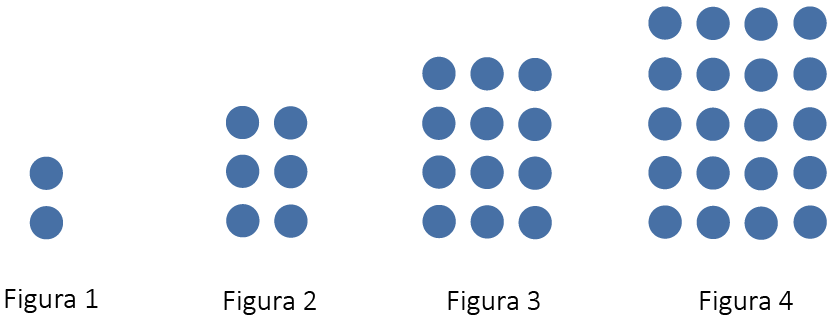
\includegraphics[width=\textwidth]{../ilustracoes/MAT5/SAEB_5ANO_MAT_figura29.png}
\end{figure}

\begin{minipage}{.5\textwidth}
\begin{escolha}
\item
  25
\item
  30
\item
  35
\item
  42
\end{escolha}
\end{minipage}
\sidetext{SAEB: Inferir os elementos ausentes em uma sequência de números naturais ordenados, objetos ou figuras.
Não há correspondência com a BNCC do quinto ano.}

\num{2} Analise com muita atenção a sequência apresentada e assinale a
alternativa que traz, de acordo com o padrão de formação, a classificação em crescente ou decrescente e
em finita ou infinita.

\begin{quote}
(66, 55, 44, 33, 22, 11)
\end{quote}

\begin{minipage}{.5\textwidth}
\begin{escolha}
\item
  Crescente e infinita.
\item
  Crescente e finita.
\item
  Decrescente e finita.
\item
  Decrescente e infinita.
\end{escolha}
\end{minipage}
\sidetext{SAEB: Inferir ou descrever atributos ou propriedades comuns que os elementos que constituem uma sequência recursiva de números naturais apresentam.
Não há correspondência com a BNCC do quinto ano.}

\num{3} Dois aplicativos exigem uma senha numérica para serem acessados.
Breno
criou a senha 6.081 para o primeiro e, para o segundo, utilizou como senha
o sucessor do sucessor do número escolhido para a primeira senha. Qual a
senha utilizada por Breno para o segundo aplicativo?

\begin{minipage}{.5\textwidth}
\begin{escolha}
\item
  6.079
\item
  6.080
\item
  6.082
\item
  6.083
\end{escolha}
\end{minipage}
\sidetext{SAEB: Inferir o padrão ou a regularidade de uma sequência de números naturais ordenados, objetos ou figuras.
Não há correspondência com a BNCC do quinto ano.}

\chapter{Medindo o mundo}
\markboth{Módulo 4}{}

\coment{Habilidade da BNCC: EF05MA19.}

\colorsec{Habilidades do SAEB}

\begin{itemize}
\item Reconhecer a unidade de medida ou o instrumento mais apropriado para
medições de comprimento, área, massa, tempo, capacidade ou temperatura.

\item Estimar/inferir medida de comprimento, capacidade ou massa de objetos,
utilizando unidades de medida convencionais ou não ou medir comprimento,
capacidade ou massa de objetos.

\item Explicar que o resultado de uma medida depende da unidade de medida utilizada.

\item Resolver problemas que envolvam medidas de grandezas (comprimento,
massa, tempo e capacidade) em que haja conversões entre as unidades mais
usuais.

\item Determinar o horário de início, o horário de término ou a duração de
um acontecimento.
\end{itemize}

\conteudo{Professor, durante todo este módulo, trabalhe com os alunos outras
unidades e medidas não tratadas nos exercícios, como
jardas, alqueires, hectares, milhas, milhas náuticas, medidas de som, entre outras.}

\begin{figure}[htpb!]
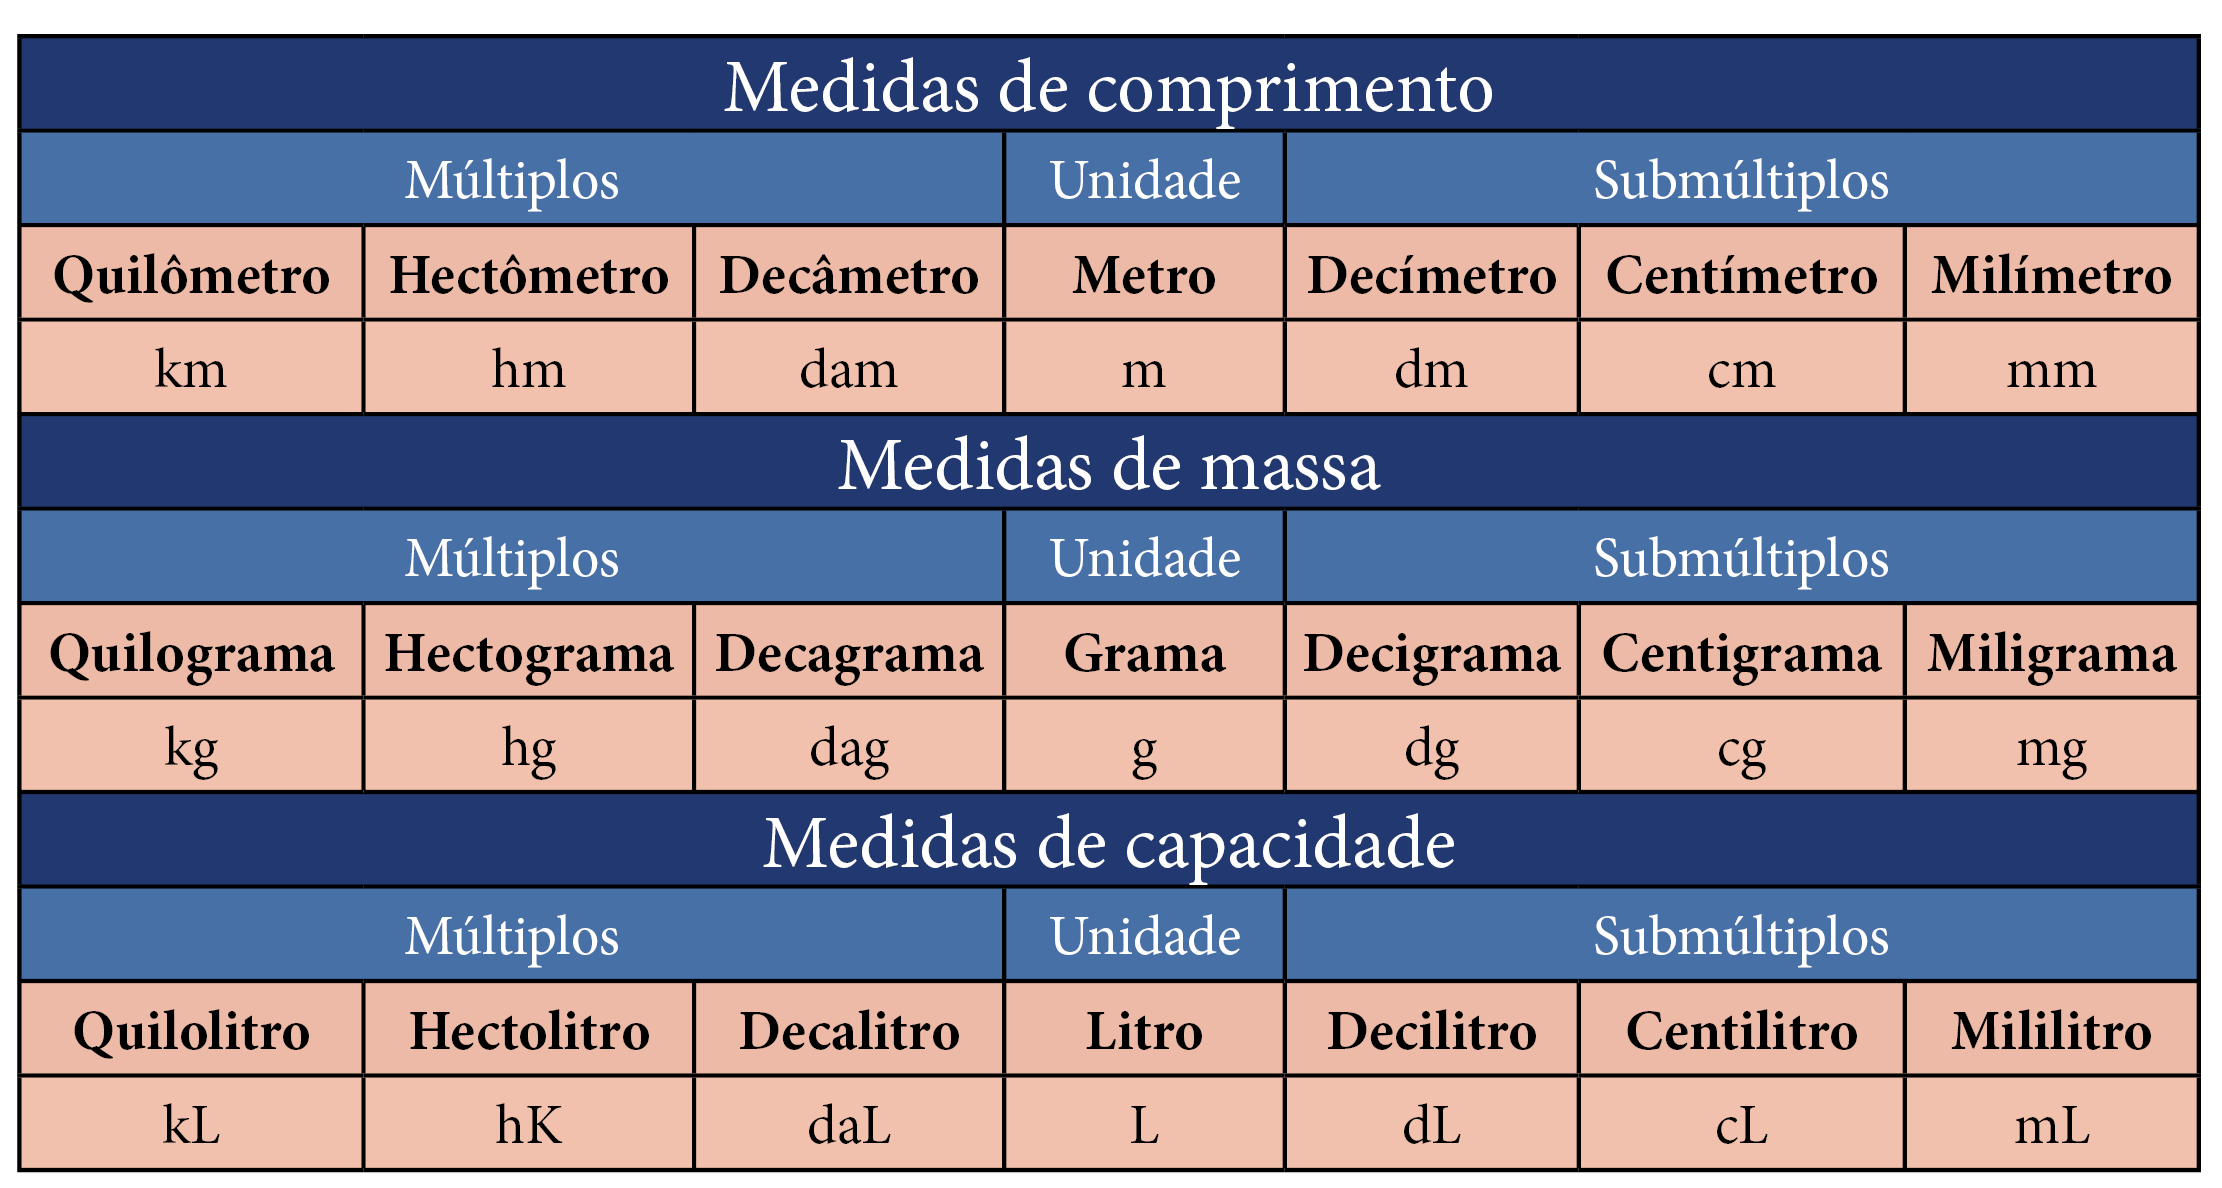
\includegraphics[width=\textwidth]{../ilustracoes/MAT5/SAEB_5ANO_MAT_figura30_1.png}
\end{figure}

\begin{figure}[htpb!]
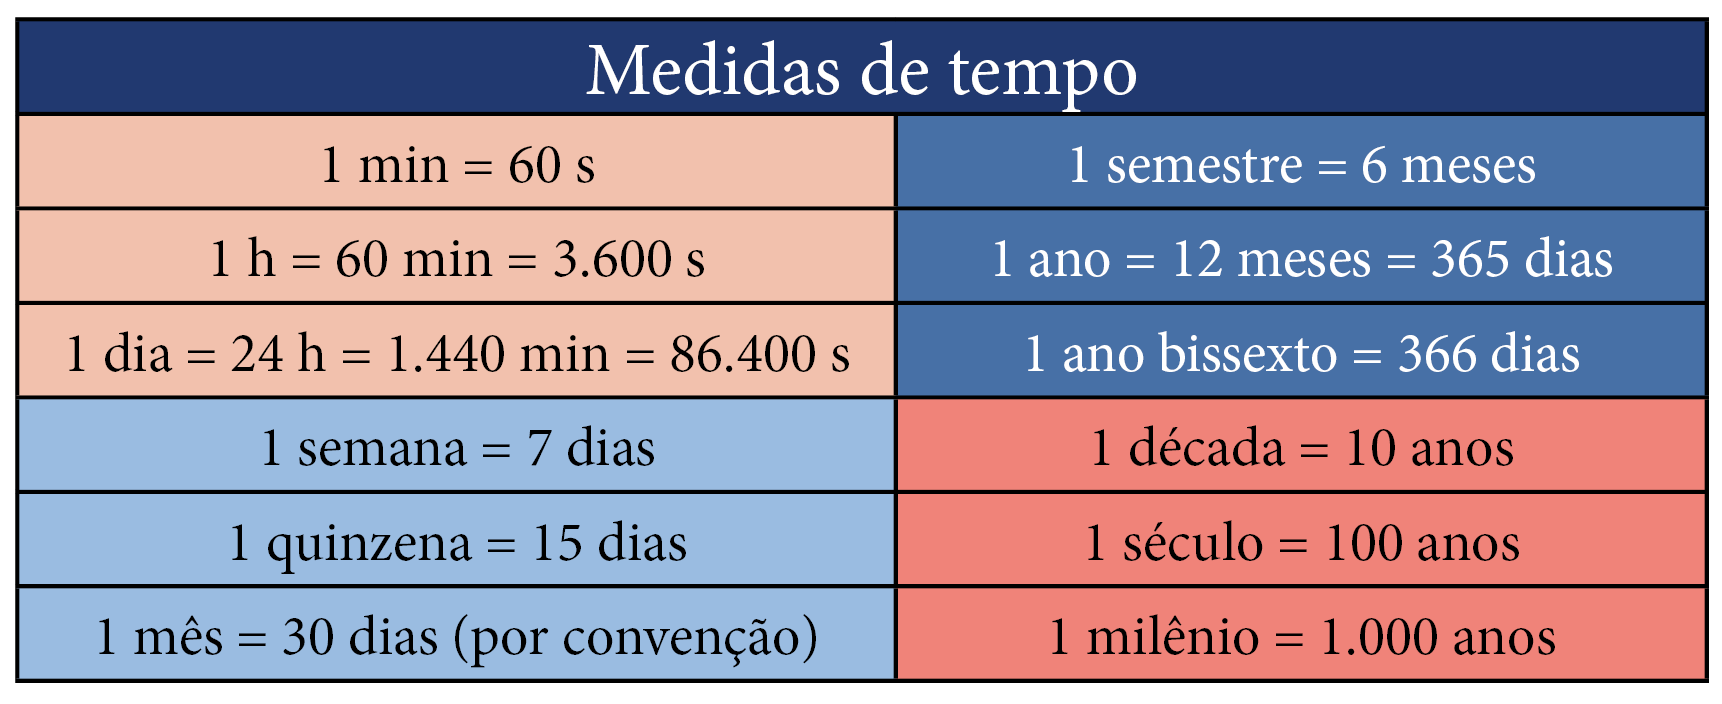
\includegraphics[width=\textwidth]{../ilustracoes/MAT5/SAEB_5ANO_MAT_figura30_2.png}
\end{figure}

\colorsec{Atividades}

\num{1} Relacione as quantidades que estão na coluna 1 com a leitura correta correspondente.

\begin{multicols}{2}
\red{1,935 kg} 

\red{2,340 km} 

\red{0,400 g} 

\red{0,35 m} 

\blue{Trinta e cinco centímetros.}

\blue{Um quilo e novecentos e trinta e cinco gramas.}

\blue{Dois quilômetros e trezentos e quarenta metros.}

\blue{Quatrocentos miligramas.}
\end{multicols}


\coment{
1.935 kg = um quilo e novecentos e trinta e cinco gramas.

2,340 km = Dois quilômetros e trezentos e quarenta metros.

0,400 g = quatrocentos miligramas.

0,35 m = trinta e cinco centímetros.}

\num{2} Relacione a primeira com a segunda coluna levando em conta qual
valor pode corresponder à medida mostrada.

\begin{multicols}{2}

Altura aproximada de uma porta (\coment{2 m})

Comprimento aproximado de um lápis (\coment{20 cm})

Comprimento médio de um quarteirão (\coment{90 m})

Comprimento aproximado de uma quadra de basquete (\coment{30 m})

\columnbreak

20 cm
 
90 m

30 m
 
2 m
\end{multicols}

\coment{Professor, explore bastante com os alunos esse senso de tamanho, pois 
é um conceito extremamente importante para eles.}

\num{3} Pinte a opção que corresponde à capacidade total de líquido que
há em:

\begin{figure}[htpb!]
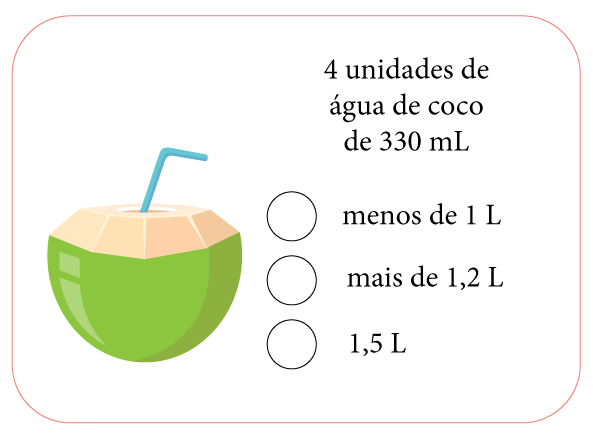
\includegraphics[width=.5\textwidth]{../ilustracoes/MAT5/SAEB_5ANO_MAT_figura31.png}
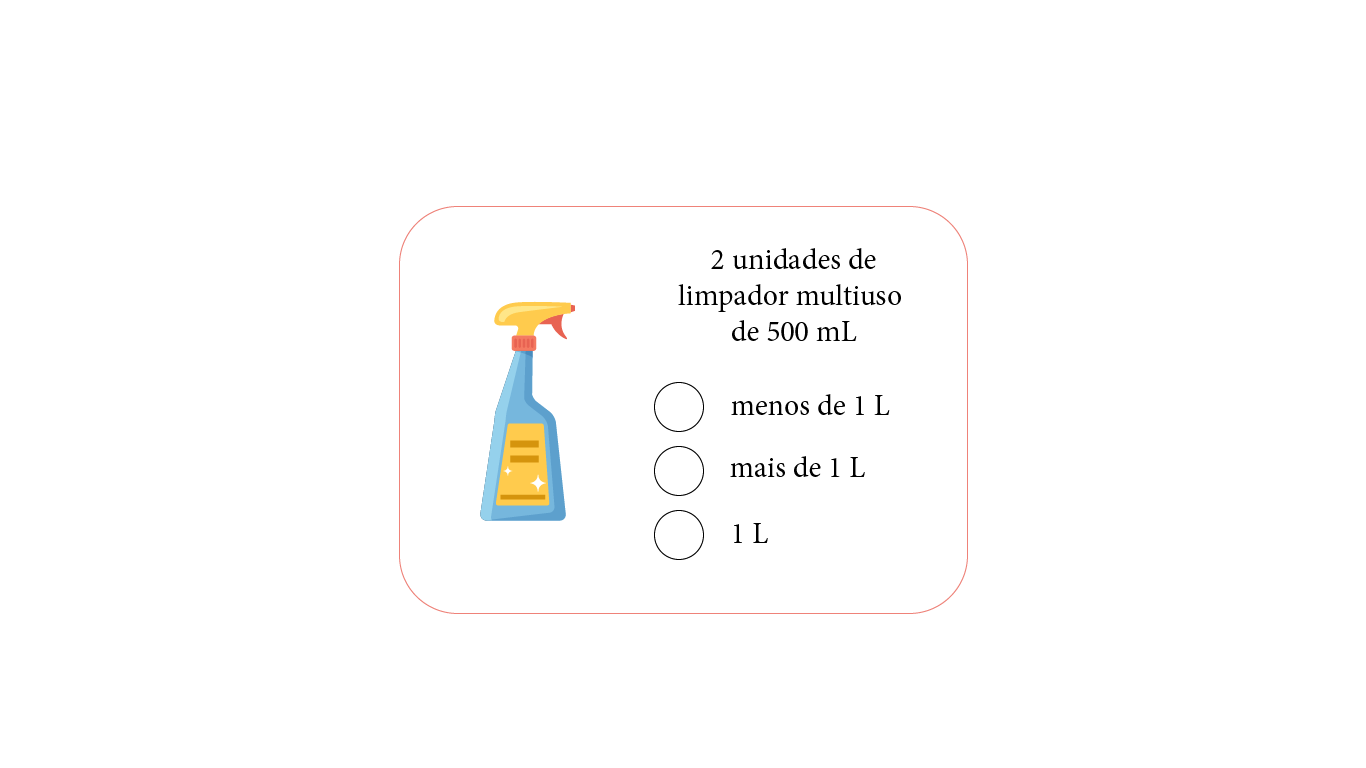
\includegraphics[width=.5\textwidth]{../ilustracoes/MAT5/SAEB_5ANO_MAT_figura31a.png}
\end{figure}

\begin{figure}[htpb!]
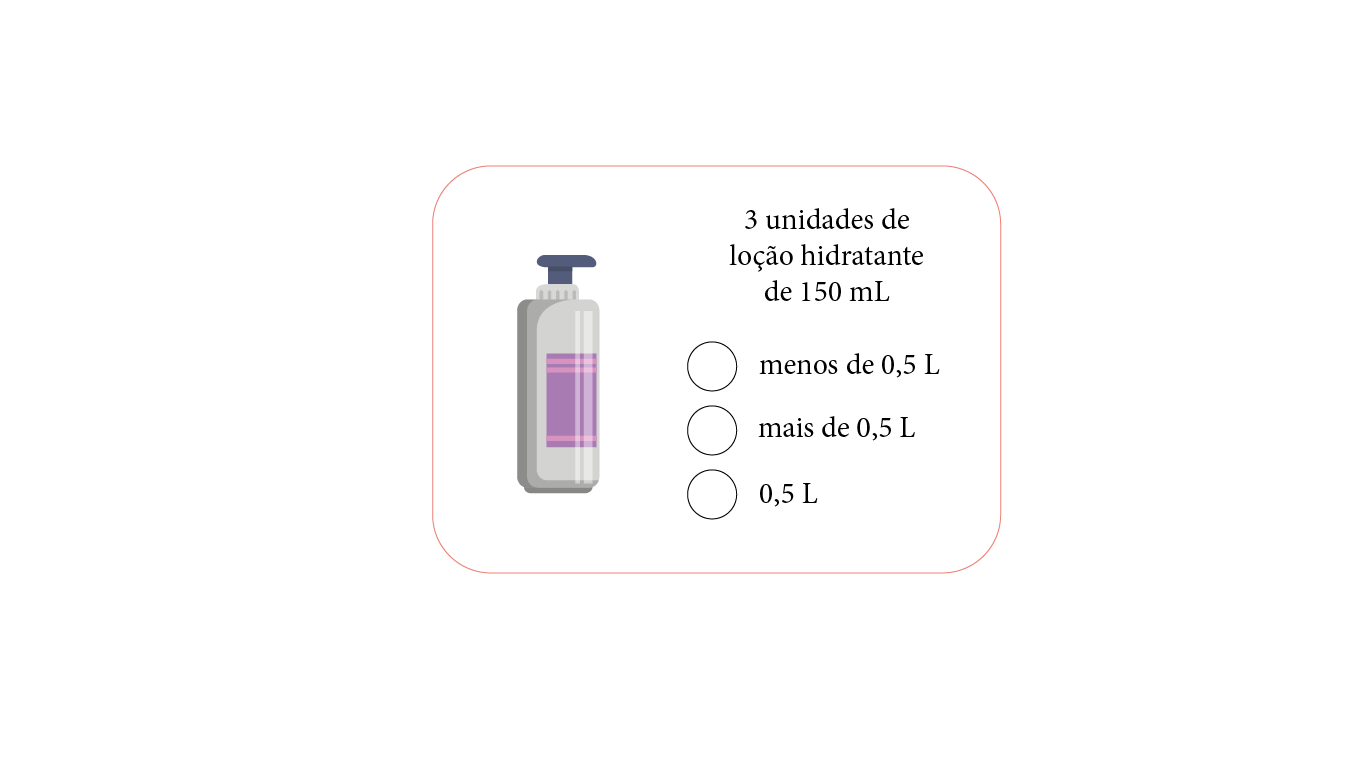
\includegraphics[width=.3\textwidth]{../ilustracoes/MAT5/SAEB_5ANO_MAT_figura31b.png}
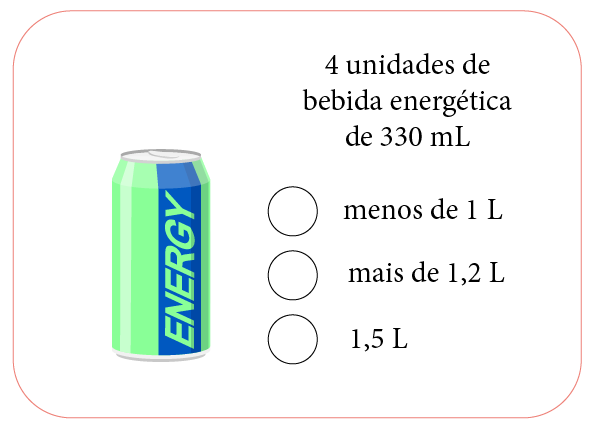
\includegraphics[width=.3\textwidth]{../ilustracoes/MAT5/SAEB_5ANO_MAT_figura31c.png}
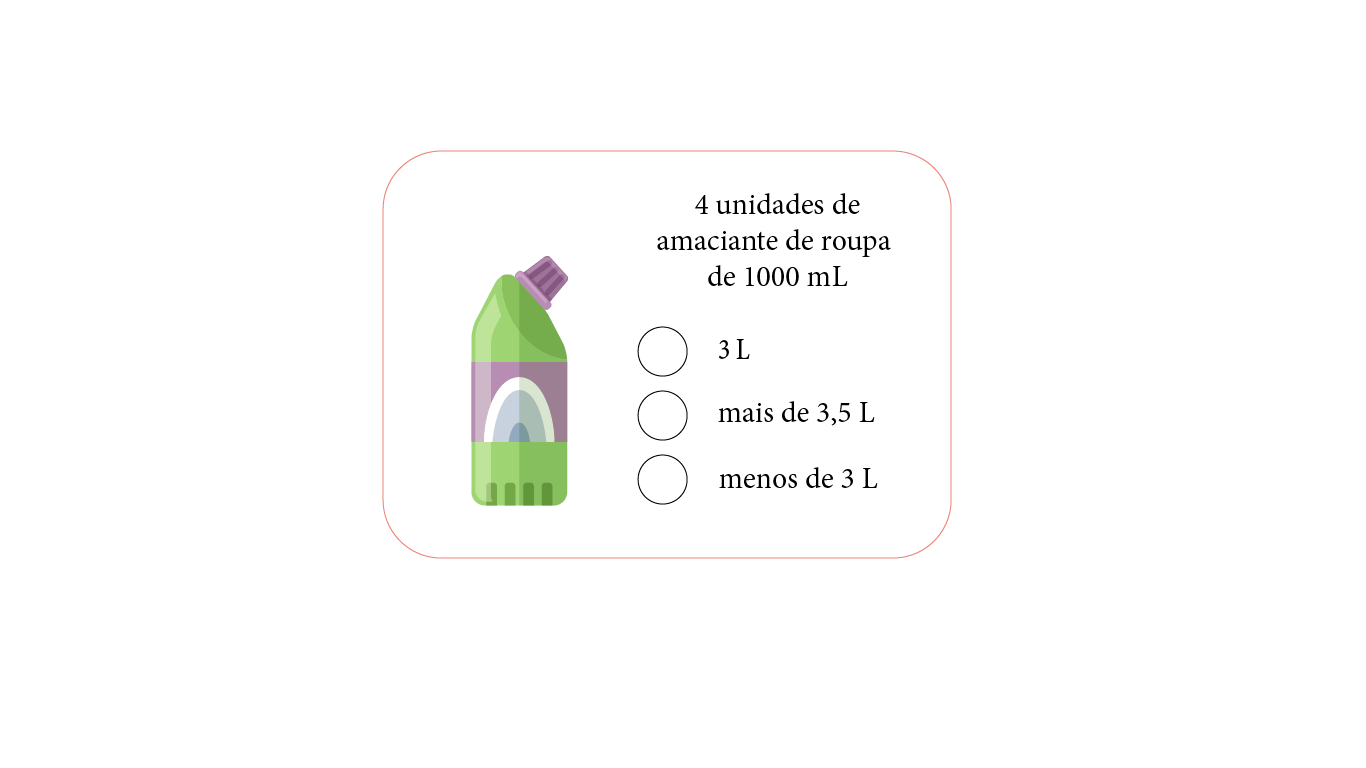
\includegraphics[width=.3\textwidth]{../ilustracoes/MAT5/SAEB_5ANO_MAT_figura31d.png}
\end{figure}


\coment{
2 unidades de limpador multiuso de 500 ml = 1 l

3 unidades de loção hidratante de 150 ml = 450 ml, que é menos que 0,5 l

4 unidades de água de coco de 330 ml = 1.320 ml = 1,32 l que é
menos do que 1,5 l

4 unidades de amaciante de roupas de 1 000 ml = 4 000 ml = 4 l, que é mais
do que 3,5 l}

\num{4} Débora decidiu estimar a medida do lápis com sua borracha.

\begin{figure}[htpb!]
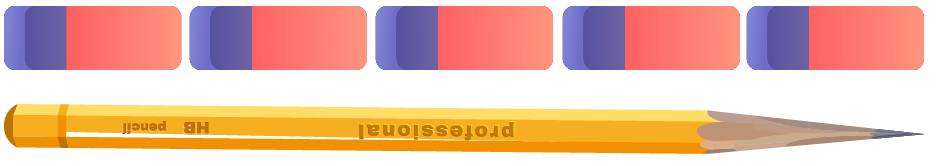
\includegraphics[width=\textwidth]{../ilustracoes/MAT5/SAEB_5ANO_MAT_figura32.png}
\end{figure}

Quantas borrachas, considerando a figura dada, aproximadamente, mede o
lápis de Débora?

\begin{escolha}
\item
  Entre 2 e 3.
\item
  Entre 4 e 5.
\item
  Entre 6 e 7.
\item
  Mais que 9.
\end{escolha}

\coment{Resposta: B.
Através da percepção de comparação de comprimentos, percebe-se que. no
comprimento de um lápis. cabem cerca de 4 a 5 borrachas conforme a figura
dada.}

\num{5} Um dos brinquedos do parque de diversões permanente de uma cidade
proíbe que crianças com uma altura menor que 1,20 m possam brincar nessa
atração. Manoel mediu sua altura e ele está com 93 cm. Quanto ele
precisa crescer para poder realizar seu sonho de andar nesse brinquedo?

\matlinhas{2}

\coment{
1,20 m = 120 cm

120 -- 93 = 23 cm

Portanto, Manoel ainda precisará crescer 23 cm para que esteja apto a brincar
nessa atração.}

\num{6} Roberto está com sintomas de dor de garganta e sua mãe decidiu levá-lo ao
médico. Chegando lá, sua temperatura foi medida e a foto do termômetro
está a seguir.

\begin{figure}[htpb!]
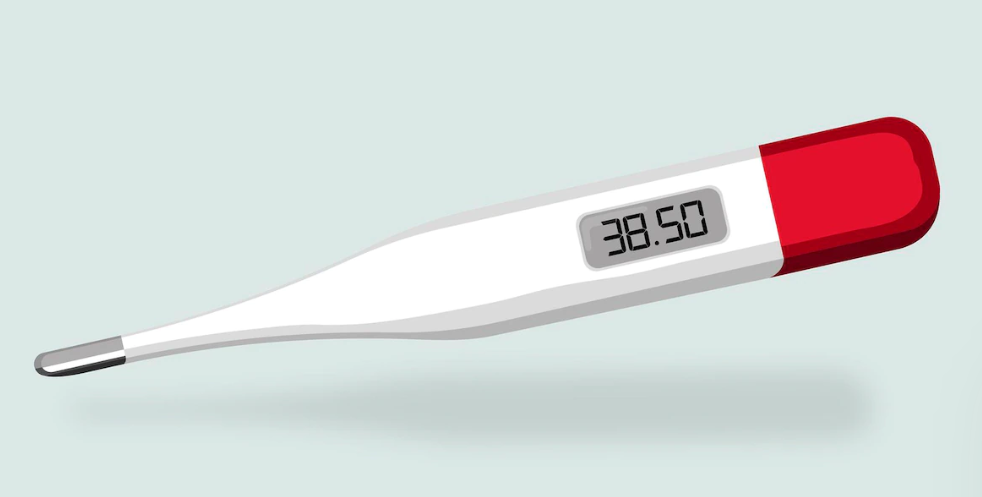
\includegraphics[width=.5\textwidth]{./imgs/mat4.png}
%https://img.freepik.com/vetores-gratis/elemento-termometro-digital-38-5-graus-celsius_53876-119949.jpg?w=1380\&t=st=1677436599~exp=1677437199~hmac=efddbcbdae2d4d75bd1e8476eee389a985a191d57800533acdff847111e69669
\end{figure}

Analisando a imagem do termômetro, podemos concluir que a temperatura de
Roberto, naquele instante, era de quanto?

\coment{38,5° C.
Observando a figura percebemos que o termômetro está marcando exatamente
38,5° C}

\num{7} Dados da prefeitura de uma determinada cidade revelam que cada
habitante, em média, produz 500 g de lixo por dia. Quantas toneladas de lixo,
aproximadamente, são produzidas, por dia, nessa cidade, que
possui uma população de 28.165 habitantes?

\matlinhas{3}

\coment{28.165 x 500 = 14.082.500 g = 14.082,50 kg = 14,0825 toneladas.}

\num{8} Para a festa de aniversário de Arthur, seu pai encomendou 24
garrafas de refrigerante. Dessas garrafas, 10 continham, cada uma, 3
litros. Nas demais garrafas, havia dois litros em cada uma. Com base
nessas informações, responda ao que se pede.

\begin{escolha}
\item
  Qual a quantidade, em mililitros, encomendada pelo pai de Arthur?

\matlinhas{3}

\item
  Se cada pessoa consumiu exatamente 400 mililitros de refrigerante e
  todo o refrigerante foi consumido durante a festa, quantas pessoas
  foram ao aniversário de Arthur?

\matlinhas{2}
\end{escolha}

\coment{
a) (10 x 3) + (14 x 2) = 30 + 28 = 58 l = 58.000 ml.
b) 58.000 : 400 = 145 pessoas compareceram à festa.}

\num{9} O comprimento de uma escrivaninha é de 1,6 m. Quantos palmos,
aproximadamente, mede a escrivaninha se, em média, um palmo tem 23 cm?

\coment{Resposta: 7.

1,6 m = 160 cm

160 : 23 = 6,95 palmos. Aproximadamente 7 palmos.}

\num{10} Uma série de televisão proporciona episódios com duração de 45
minutos. Se Jorge terminou de assistir a um desses episódios às 18 horas, qual
foi o horário em que ele começou a assistir a esse episódio, considerando que tenha assistido
no início ao fim sem parar nenhuma vez?

\matlinhas{2}

\coment{Ele começou a assistir ao episódio às 17 horas e 15 minutos, pois, se a esse
horário somarmos a duração do episódio, que é de 45 minutos, teremos o
horário final, que foi às 18 horas.}

\section{Treino}

\num{1} Reinaldo foi contratado por uma empresa que possui um horário bem
rígido e semanal que deve ser cumprido corretamente. No período da manhã,
ele deve cumprir 4 horas e 30 minutos de trabalho. Qual será o horário em que
Reinaldo sairá para almoçar nesses dias?

\begin{longtable}[]{@{}lll@{}}
\toprule
& Entrada & Saída\tabularnewline
\midrule
\endhead
Manhã & 8:00 & ?\tabularnewline
Tarde & 14:00 & 17:30\tabularnewline
\bottomrule
\end{longtable}

\begin{minipage}{.5\textwidth}
\begin{escolha}
\item
  11:00
\item
  11:30
\item
  12:00
\item
  12:30
\end{escolha}
\end{minipage}
\sidetext{SAEB: Determinar o horário de início, o horário de término ou a duração de um acontecimento.
BNCC: EF05MA19 -- Resolver e elaborar problemas envolvendo medidas das grandezas comprimento,
área, massa, tempo, temperatura e capacidade, recorrendo a transformações entre as unidades
mais usuais em contextos socioculturais.}

\num{2} Em uma receita médica que Marcela recebeu, o médico recomenda que ela tome um xarope 3
vezes ao dia e que, a cada vez, ela tome a quantidade de 10 ml. Isso deve se repetir durante 7
dias. Um frasco do remédio contém 100 ml. Sendo assim, qual a quantidade
de frascos que a mãe de Marcela terá que comprar para que todo o
tratamento seja concluído?

\begin{minipage}{.5\textwidth}
\begin{escolha}
\item
  1
\item
  2
\item
  3
\item
  4
\end{escolha}
\end{minipage}
\sidetext{SAEB: Reconhecer a unidade de medida ou o instrumento mais apropriado para medições de comprimento, área, massa, tempo, capacidade ou temperatura.
BNCC: EF05MA19 -- Resolver e elaborar problemas envolvendo medidas das grandezas comprimento,
área, massa, tempo, temperatura e capacidade, recorrendo a transformações entre as unidades
mais usuais em contextos socioculturais.}

\num{3} Vicente teve que fazer uma viagem para fechar um grande negócio. Seu
voo saiu do aeroporto às 10 horas e 42 minutos e chegou ao seu destino
às 14 horas e 8 minutos. Qual foi o tempo de duração do voo?

\begin{minipage}{.5\textwidth}
\begin{escolha}
\item
  12.300 segundos
\item
  9.542 segundos
\item
  5.364 segundos
\item
  2.500 segundos
\end{escolha}
\end{minipage}
\sidetext{SAEB: Determinar o horário de início, o horário de término ou a duração de um acontecimento.
BNCC: EF05MA19 -- Resolver e elaborar problemas envolvendo medidas das grandezas comprimento,
área, massa, tempo, temperatura e capacidade, recorrendo a transformações entre as unidades
mais usuais em contextos socioculturais.}


\chapter{Áreas, espaços, tamanhos}
\markboth{Módulo 5}{}

\colorsec{Habilidades do SAEB}

\begin{itemize}
\item Medir ou comparar perímetro ou área de figuras planas desenhadas em
malha quadriculada.

\item Identificar horas em relógios analógicos ou associar horas em relógios
analógicos e digitais.

\item Resolver problemas que envolvam perímetro de figuras planas.

\item Resolver problemas que envolvam área de figuras planas.
\end{itemize}

\conteudo{Professor, explore bastante os conceitos de identificação de horas e
relógio analógico e também a utilização da malha quadriculada para
identificação do perímetro e de área de figuras planas.

Ampliação: é o processo que realizamos quando queremos aumentar algo (como figuras planas, por exemplo) sem que suas características essenciais
sejam alteradas.

A figura representada teve seus lados dobrados e manteve as mesmas
características. Observe.

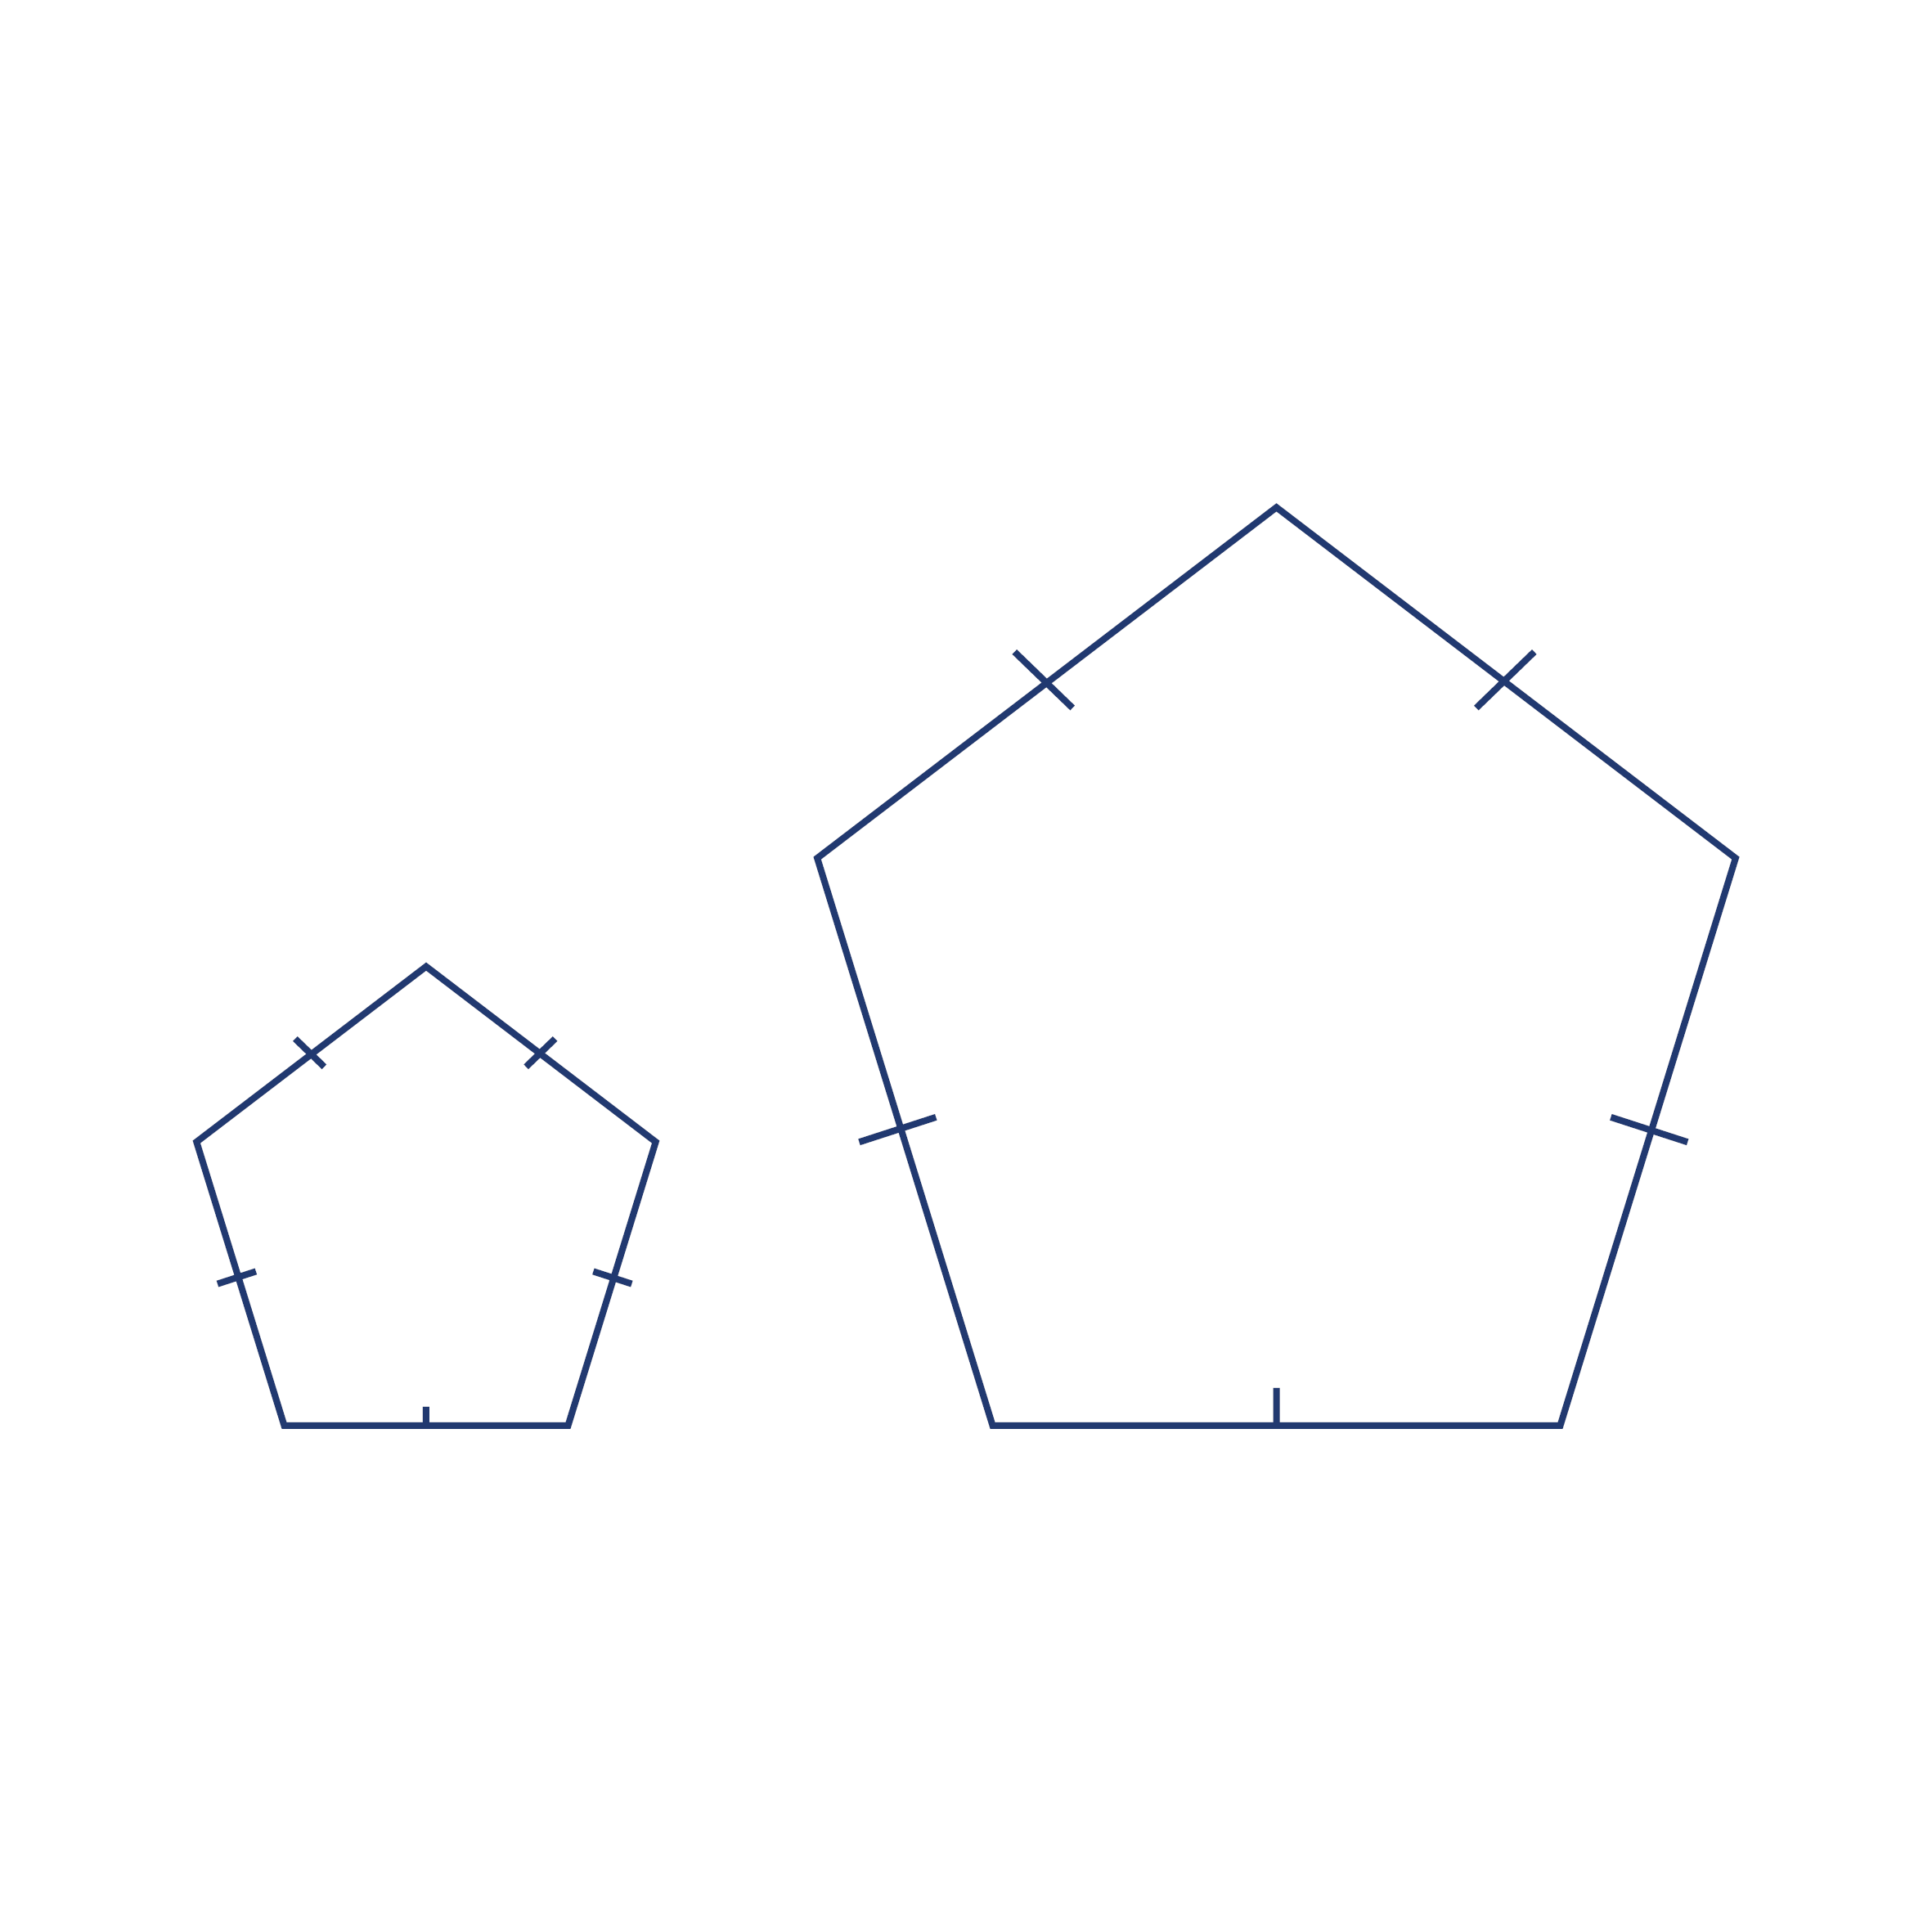
\includegraphics[width=\textwidth]{../ilustracoes/MAT5/SAEB_5ANO_MAT_figura33.png}

Redução: é o processo que realizamos quando queremos diminuir algo (como figuras planas, por exemplo) sem que suas características essenciais
sejam alteradas.

A figura representada teve seus lados divididos pela metade e manteve as mesmas
características. Observe.

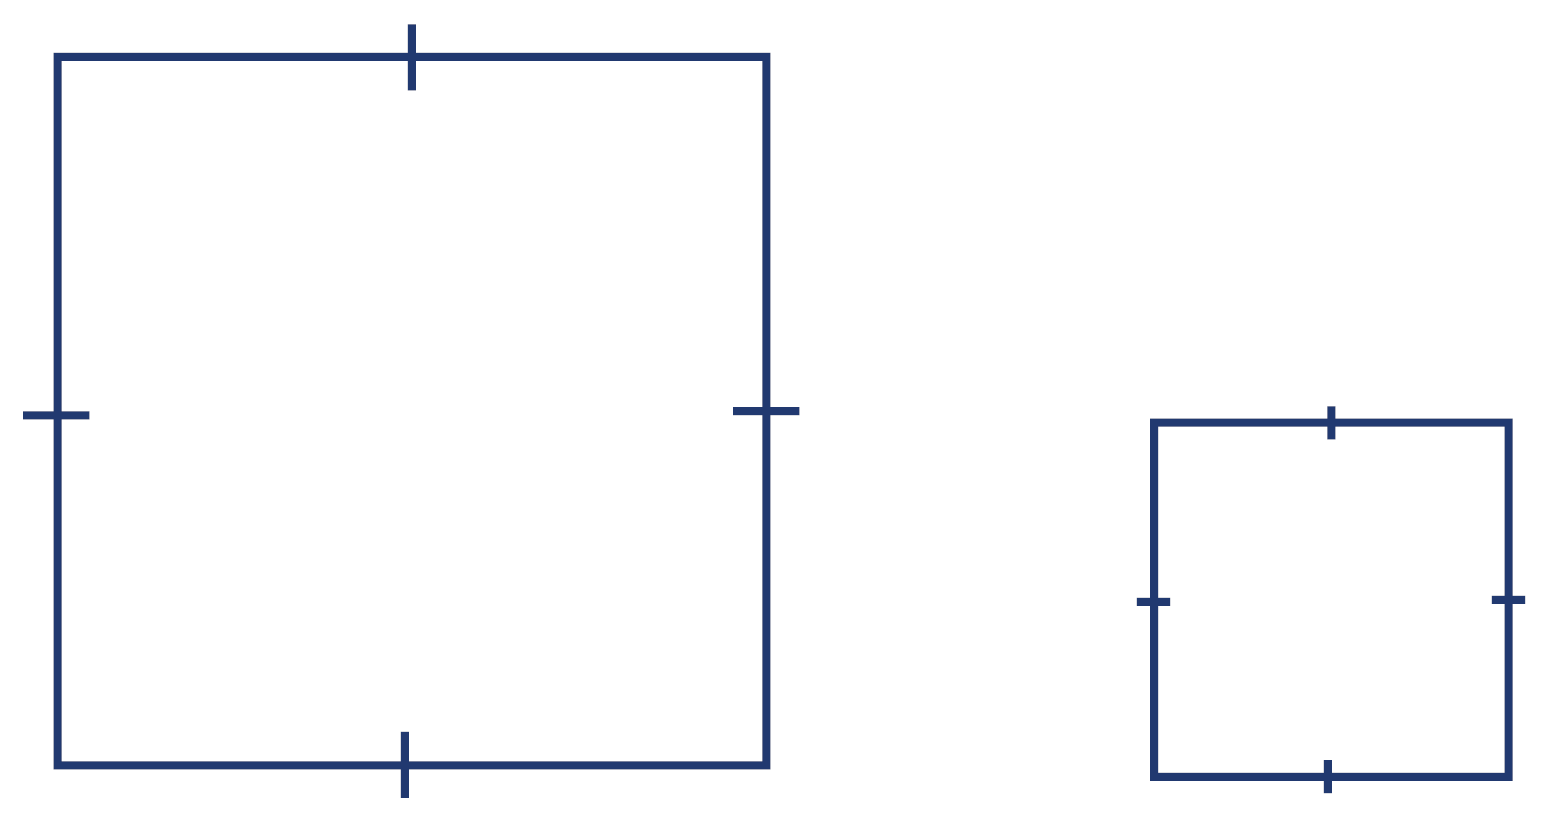
\includegraphics[width=\textwidth]{../ilustracoes/MAT5/SAEB_5ANO_MAT_figura34.png}

Muitas vezes recorremos ao auxílio de malhas quadriculadas para nos
ajudar nesse processo.}

\colorsec{Atividades}

\num{1} Renato, aos finais de semana, anda de bicicleta ao redor da praça
que fica no bairro em que mora.

\begin{figure}[htpb!]
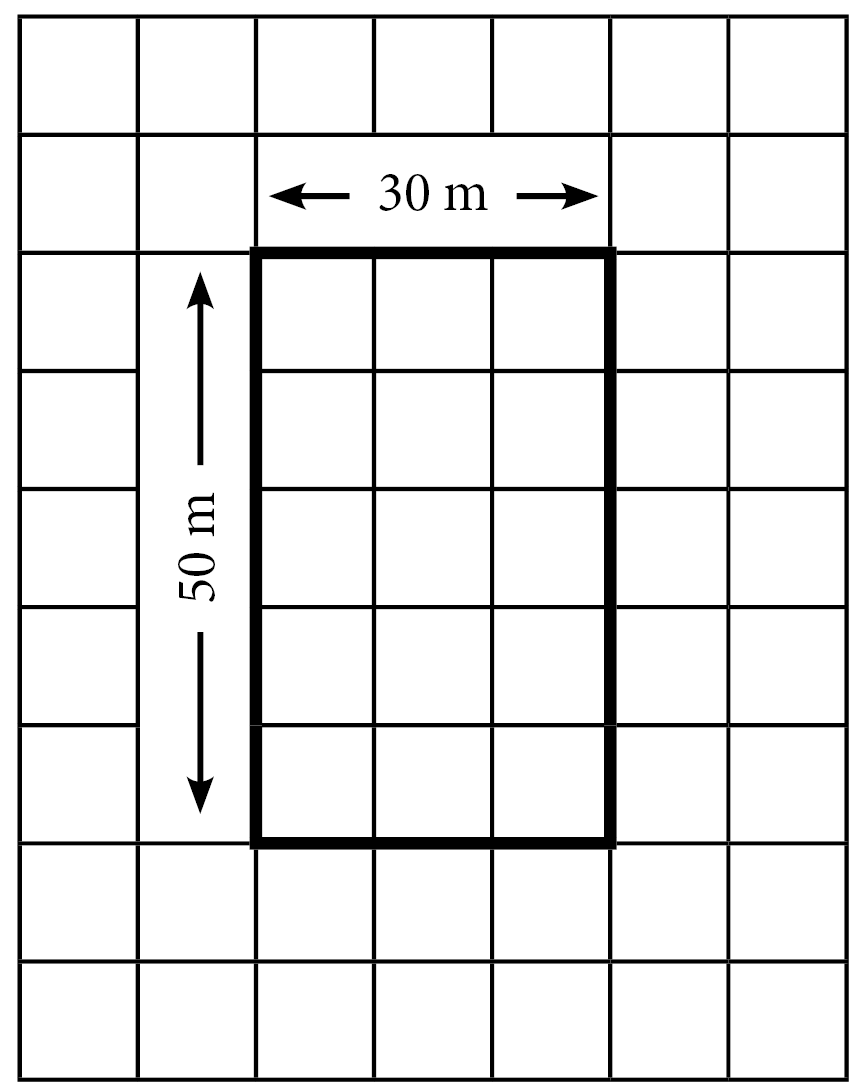
\includegraphics[width=\textwidth]{../ilustracoes/MAT5/SAEB_5ANO_MAT_figura35.png}
\end{figure}

Se ele der duas voltas completas ao redor da praça, ele percorrerá qual
distância?

\matlinhas{2}

\coment{(2 x 30 + 2 x 50) x 2 = 320 m

Professor, sempre que possível, estimule a montagem da expressão para que
os alunos comecem a se acostumar.}

\num{2} Em uma atividade escolar a professora Helena forneceu uma figura e
seus alunos Ana, Rosa, Bernardo e Daiane deveriam realizar uma ampliação. Após algum tempo, os alunos entregaram seus desenhos.

\begin{figure}[htpb!]
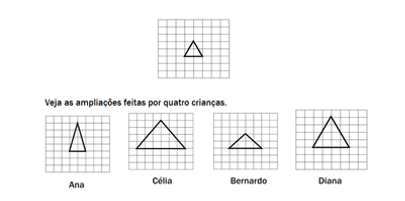
\includegraphics[width=.5\textwidth]{./imgs/mat5.png}
\end{figure}
% Construir uma figura conforme a anterior de acordo com os padrões do projeto.
% Colocar no lugar de Célia e Diana, os nomes Rosa e Daiane respectivamente.

Quem ampliou corretamente a imagem foi

\begin{escolha}
\item
  Ana.
\item
  Rosa.
\item
  Bernardo.
\item
  Daiane.
\end{escolha}

\coment{Resposta: Daiane, pois foi a única que manteve a proporcionalidade durante o
processo de ampliação.

Professor, devemos reforçar e discutir com os alunos os conceitos e
regras de ampliação e de redução.}

\num{3} Leandro resolveu cobrir de azuleijos o fundo de sua piscina, de tal
forma que apareça, nesse fundo, a letra inicial do nome de seu filho,
Arnaldo. Sabendo-se que cada quadradinho corresponde a um azuleijo,
quantos azuleijos foram utilizados para cobrir a letra inicial do nome
de seu filho?

\begin{figure}[htpb!]

\includegraphics[width=\textwidth]{../ilustracoes/MAT5/SAEB_5ANO_MAT_figura37.png}
\end{figure}


\coment{Resposta: 14.
Realizando a contagem do número de quadradinhos que formam a letra A,
percebemos que são 14 quadradinhos.}

\num{4} A entrada de um edifício está sendo reformada de tal forma que se
criem duas hortas comunitárias nas laterais; o restante do piso será coberto por um revestimento ecológico que permite a entrada da água da chuva no solo. Veja
a figura:

\begin{figure}[htpb!]
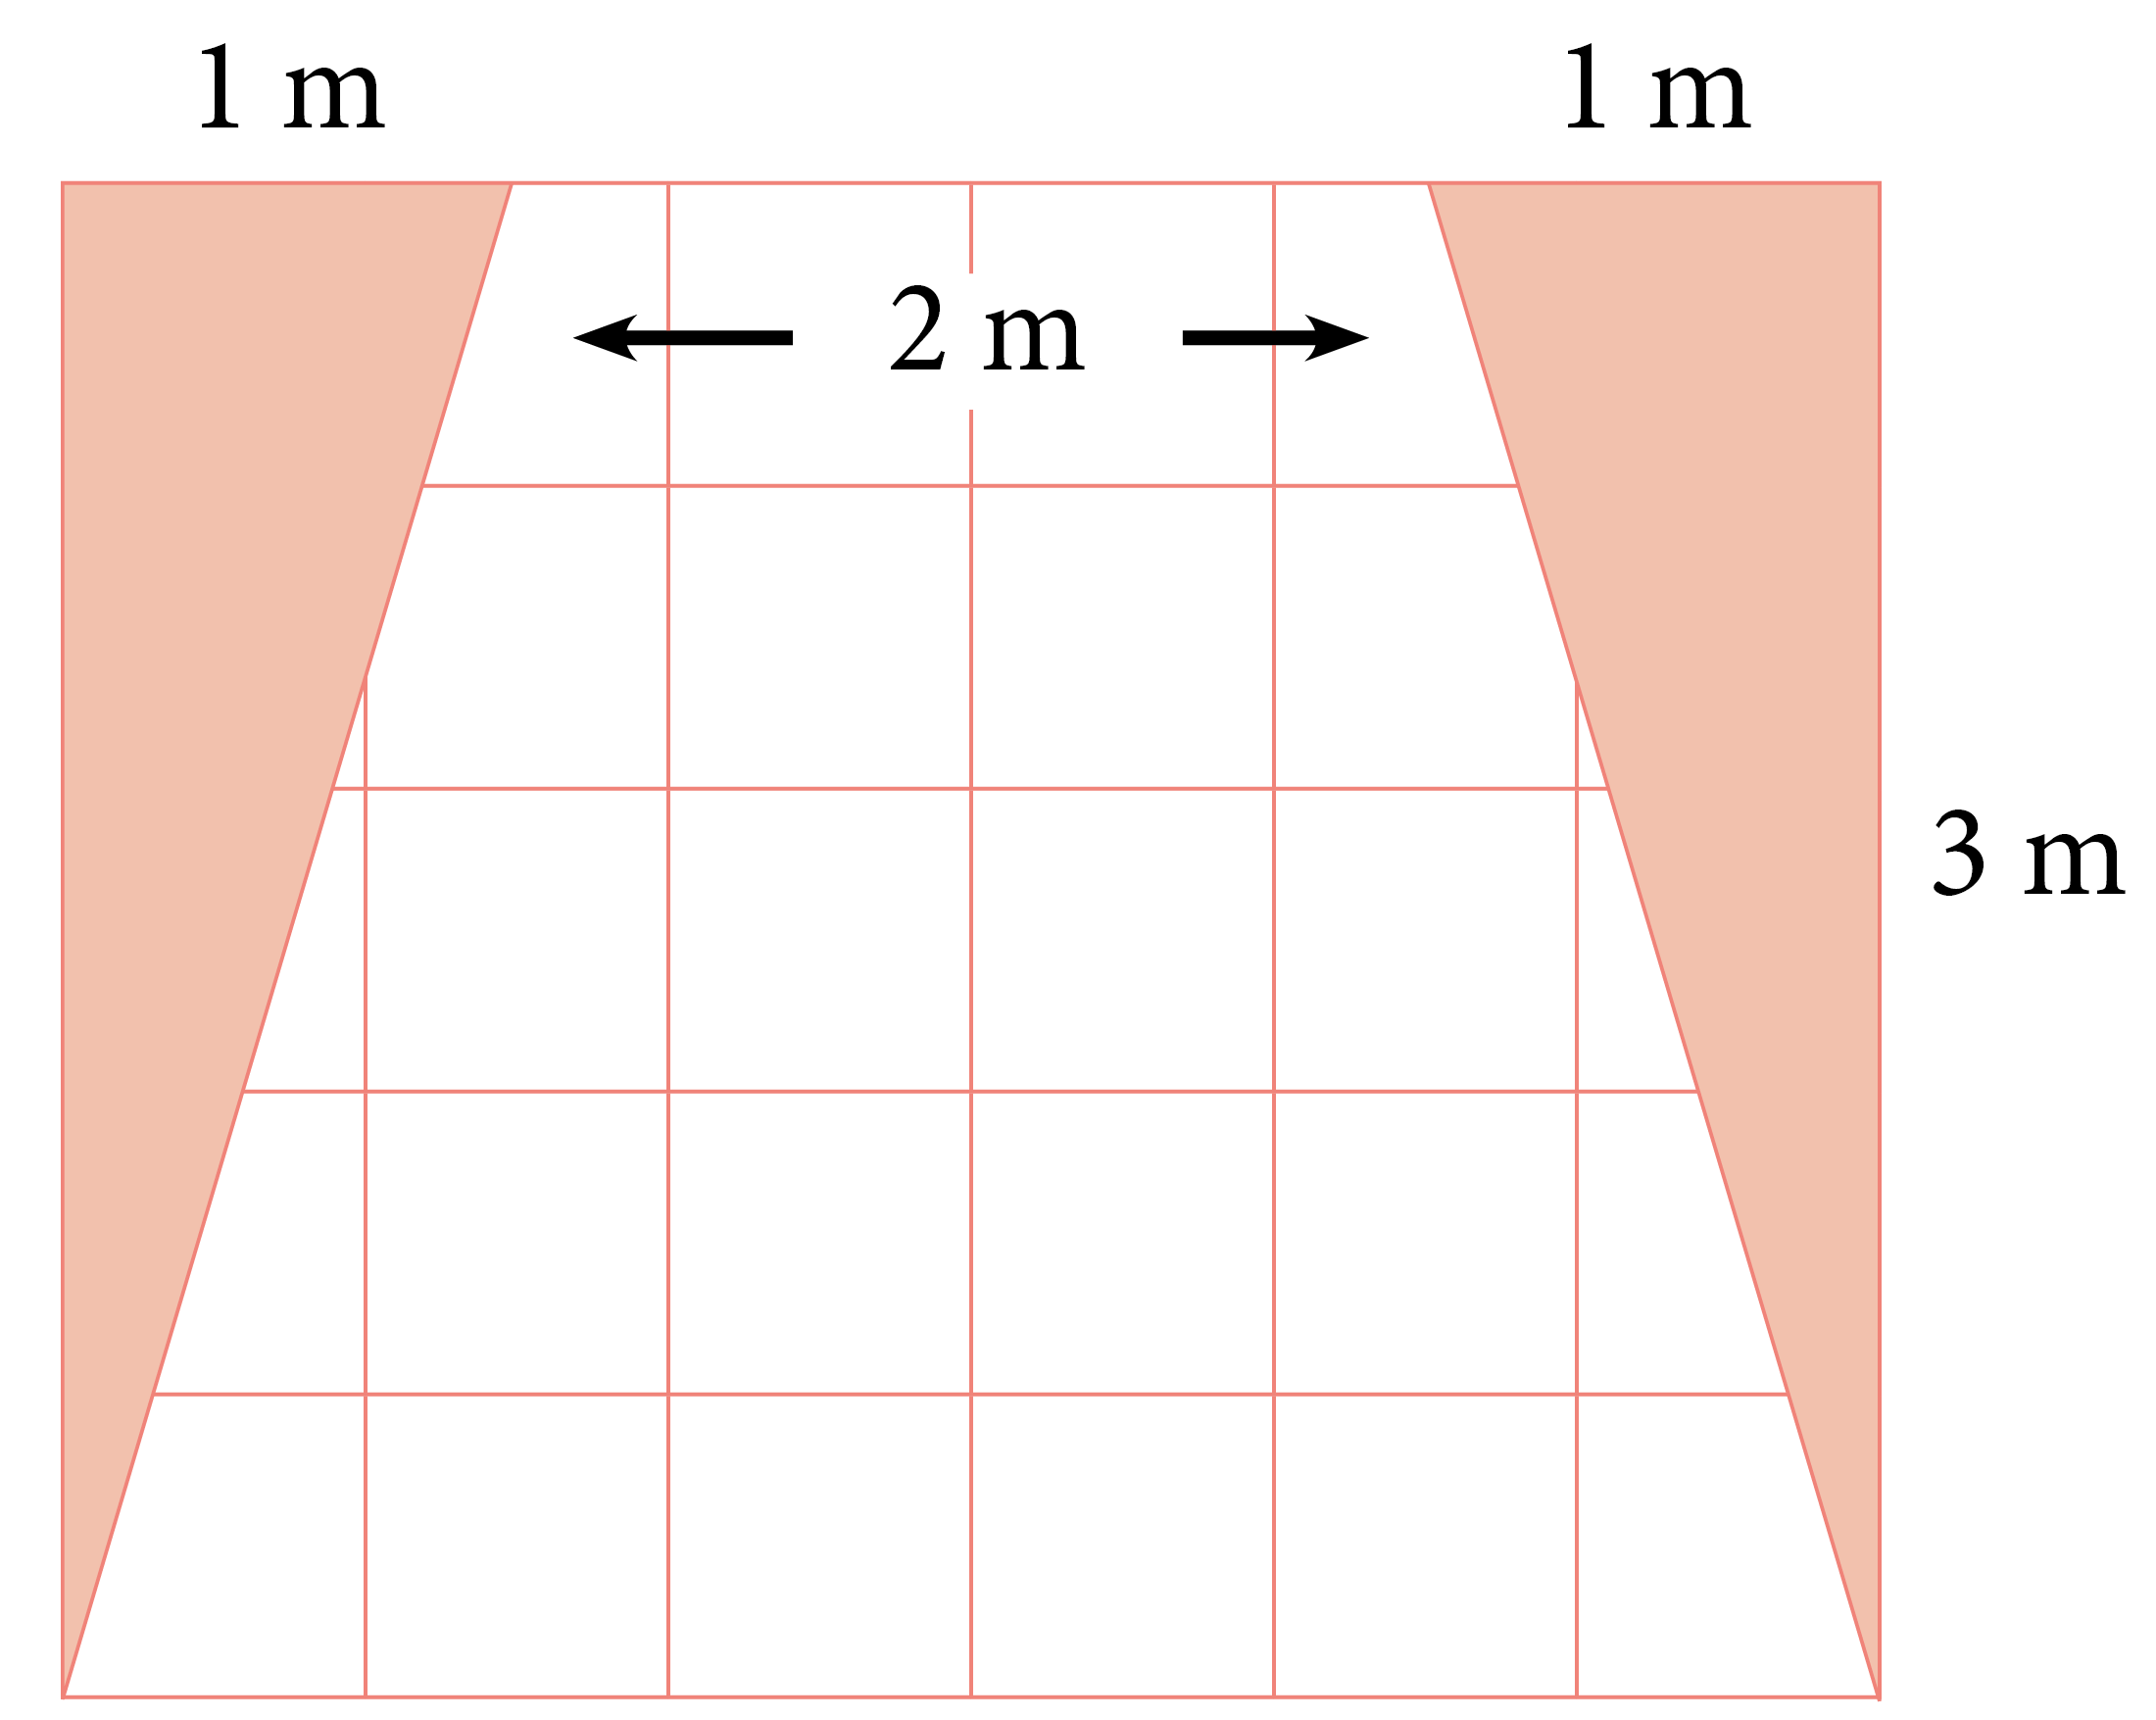
\includegraphics[width=\textwidth]{../ilustracoes/MAT5/SAEB_5ANO_MAT_figura38.png}
\end{figure}

Estime a área que será destinada às duas hortas comunitárias.

\matlinhas{3}

\coment{
Podemos efetuar o cálculo correto de área: 2 x [(1 x 3)/2] = 3 metros
quadrados.
Mas, como o exercício pede para estimar, pode-se simplesmente
contar o número de quadradinhos que as áreas destinadas às hortas
ocuparão.

Professor, devemos estimular os dois cálculos, principalmente o segundo,
pois foge um pouco das formas tradicionais de cálculo e aguça percepção.}

\num{5} Os desenhos representam os formatos, inicial  final, de uma praça que será construída em uma
área central de uma cidade. Inicialmente a previsão era de uma praça
pequena, mas, como a prefeitura conseguiu uma área maior ao lado da
primeira, optou-se por realizar a construção de uma praça maior.

\begin{figure}[htpb!]
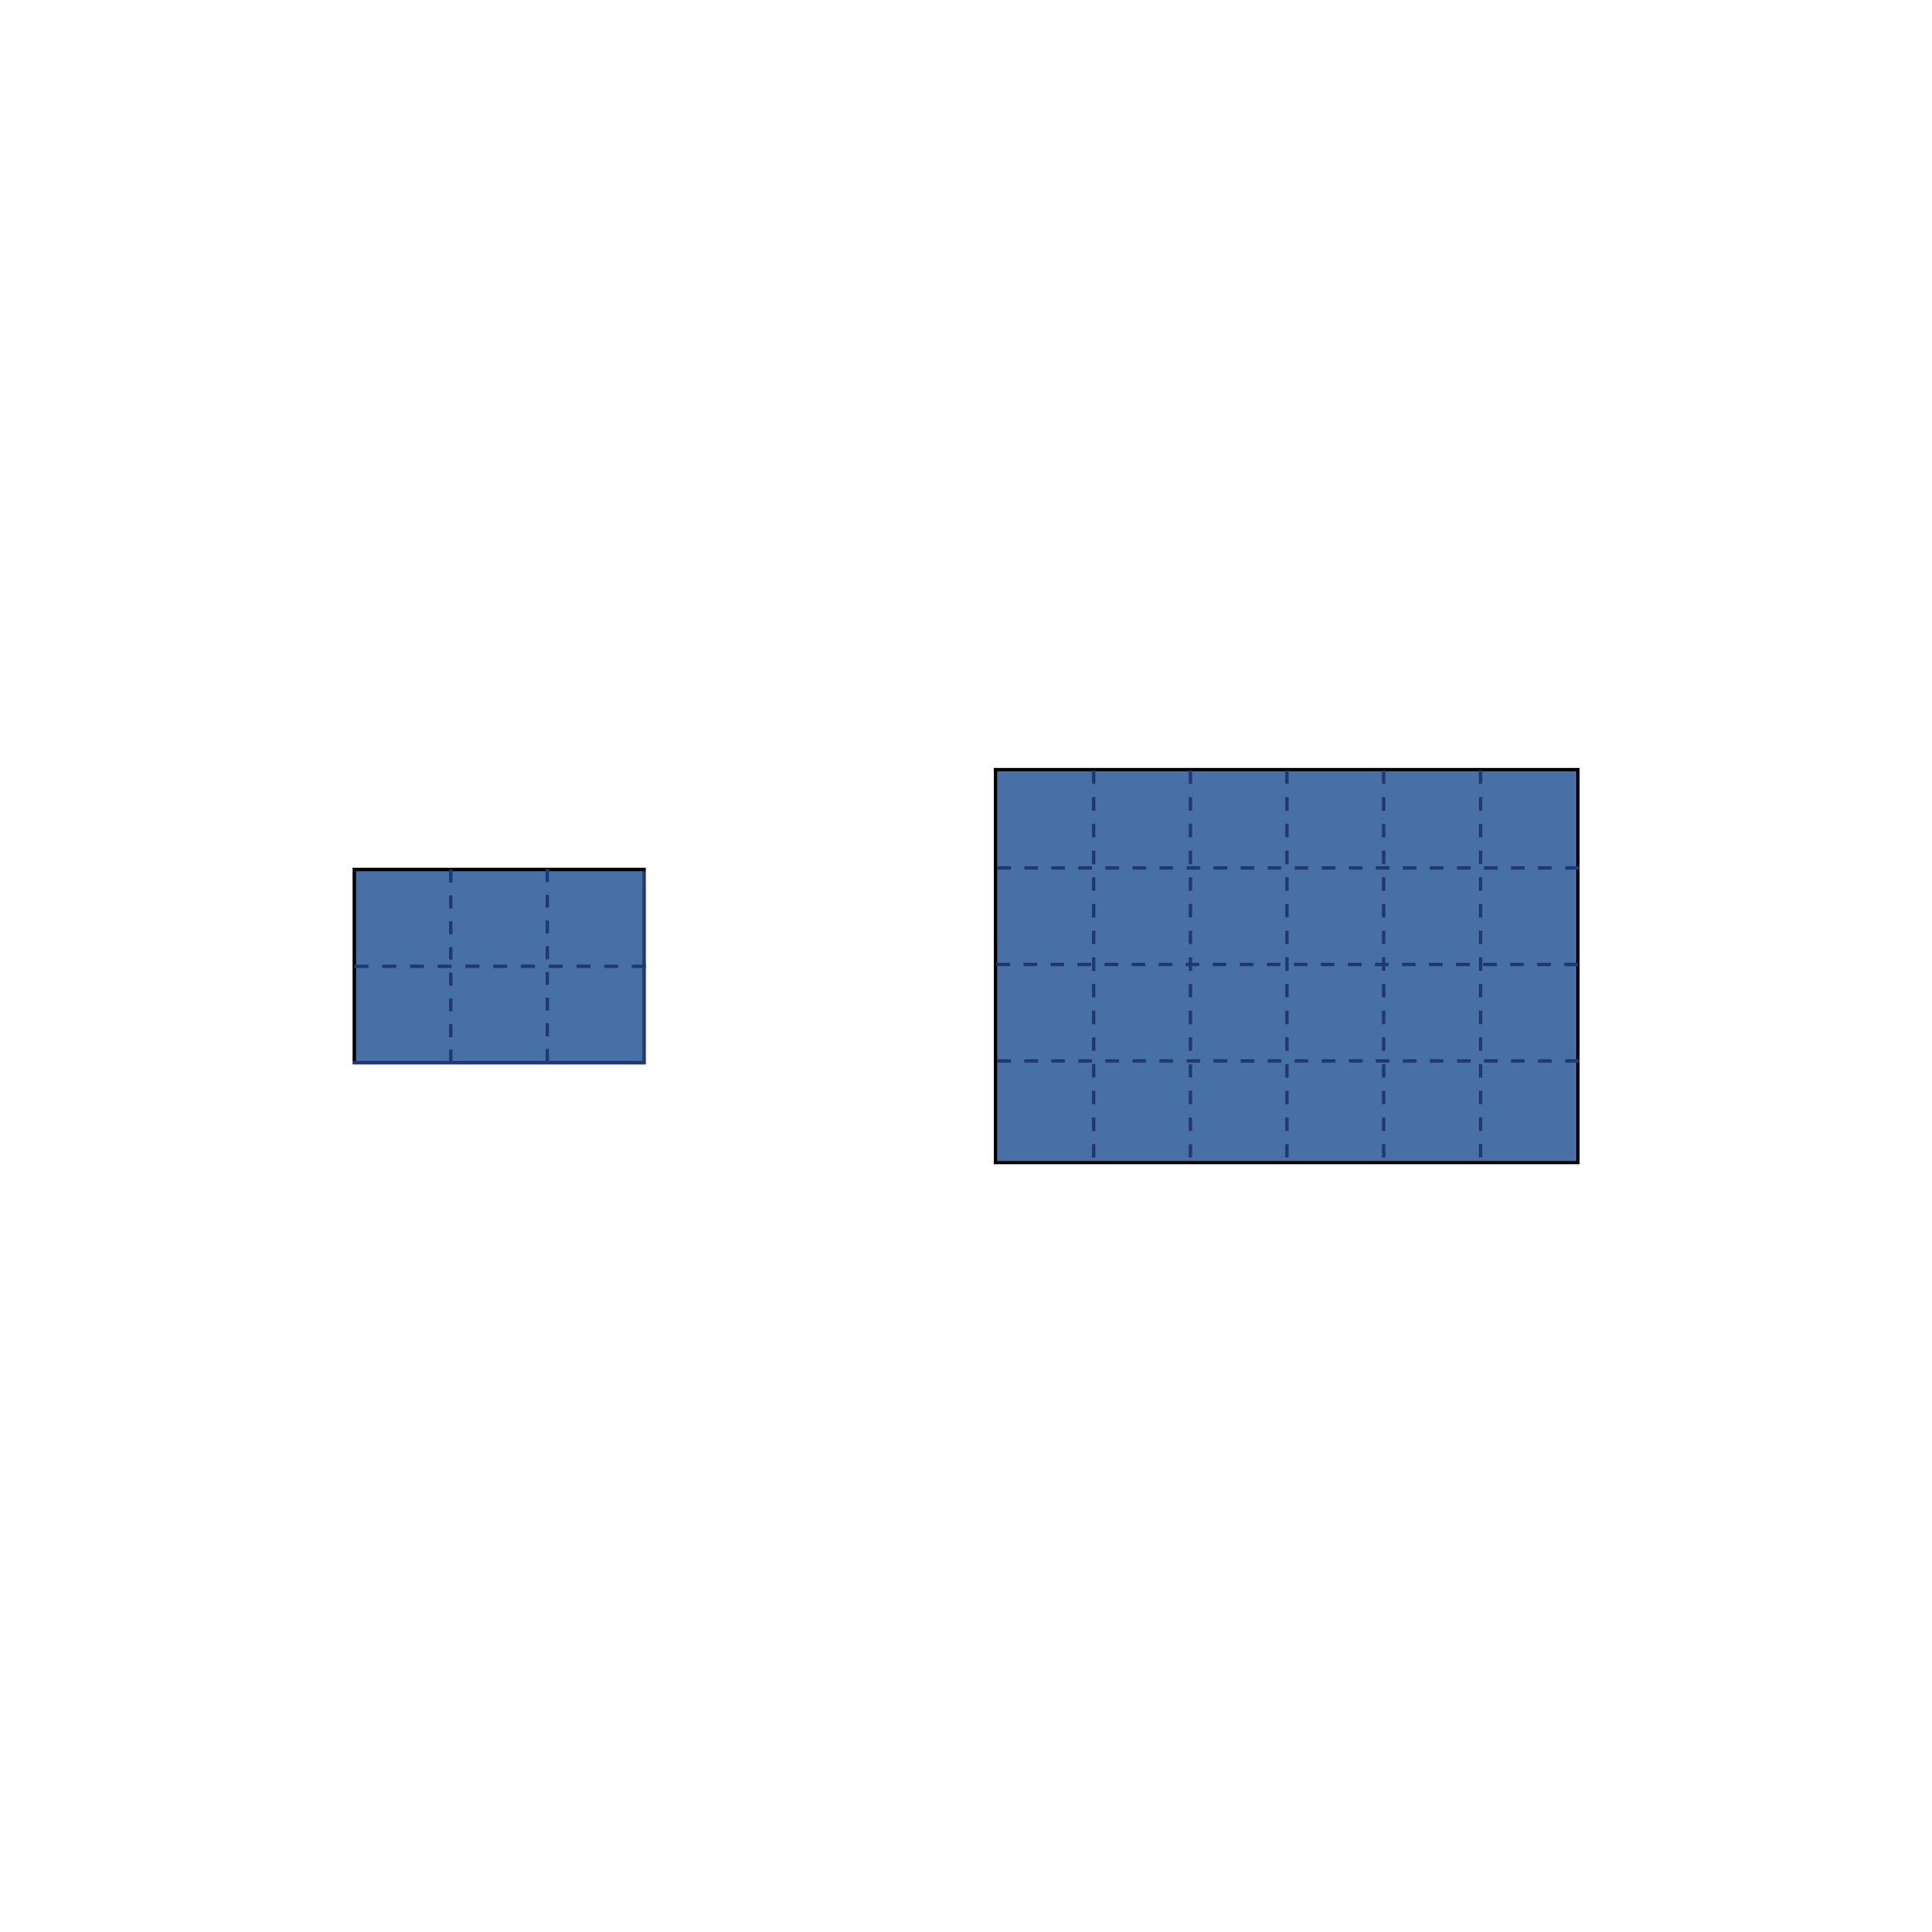
\includegraphics[width=\textwidth]{../ilustracoes/MAT5/SAEB_5ANO_MAT_figura39.png}
\end{figure}

Sendo assim, a nova praça terá, com relação à praça que se
desejava construir iniciamente, uma área

\begin{escolha}
\item
  2 vezes maior.
\item
  3 vezes maior.
\item
  4 vezes maior.
\item
  5 vezes maior.
\end{escolha}

\coment{Resposta: C.
A praça menor teria 6 quadradinhos preenchendo sua área, enquanto a
grande terá 24 quadradinhos; sendo assim, a área da praça maior é
quatro vezes a área da praça menor.}

\num{6} Observando atentamente as figuras, pode-se perceber que a figura com a menor área é:

\begin{figure}[htpb!]
\includegraphics[width=\textwidth]{../ilustracoes/MAT5/SAEB_5ANO_MAT_figura40.png}
\end{figure}


\coment{
A figura 2, composta por 4 quadradinhos.

A figura 1 é composta por 6 quadradinhos.
A figura 3 é composta por 5 quadradinhos.
A figura 4 é composta por 7 quadradinhos.

Como os quadradinhos são de mesmo tamanho, pode-se concluir que a figura
que possui a menor área é a figura 2, por ser composta por um número
menor de quadradinhos.

Professor, explore bastante esse conceito de percepção por meio da divisão
em pedaços menores de mesma medida, estimulando o senso de
comparação.}

\num{7} Um arquiteto fez um primeiro esboço de uma construção no formato de
cruz que teria que executar.

\begin{figure}[htpb!]
\includegraphics[width=\textwidth]{../ilustracoes/MAT5/SAEB_5ANO_MAT_figura41.png}
\end{figure}

Mas, no projeto final, todos os lados foram reduzidos à metade. Qual das
figuras a seguir representa a nova construção em cruz?

\begin{figure}[htpb!]
\includegraphics[width=.5\textwidth]{./imgs/mat6.png}
\end{figure}
%Construir uma figura conforme a anterior de acordo com os padrões do projeto.

\coment{Figura A.
Reduzindo todos os lados pela metade e mantendo-se a proporção, conclui-se
que a figura correta é a representada na alternativa A.}

\num{8} Na malha quadriculada, cada quadrado representa uma área de
20 metros quadrados.

\begin{figure}[htpb!]
\includegraphics[width=\textwidth]{../ilustracoes/MAT5/SAEB_5ANO_MAT_figura43.png}
\end{figure}

Qual área da malha quadriculada a figura destacada ocupa?

\reduline{Realizando a contagem de quadradinhos que preenchem a figura, chega-se à conclusão de que,
que para o preenchimento dela, são necessários 16 quadradinhos.
Portanto, 16 x 20 = 320 metros quadrados.\hfill}

\num{9} Gabriel achou nas coisas guardadas de seu irmão mais velho a
seguinte malha quadriculada com letras destacadas:

\begin{figure}[htpb!]
\includegraphics[width=.5\textwidth]{./imgs/mat7.png}
\end{figure}
%Construir uma figura conforme a anterior de acordo com os padrões do projeto.

Dentre elas existem duas que ocupam superfícies de mesmo tamanho, que são

  A e E


\coment{Resposta: A e E.
Letra A: 14 quadradinhos.
Letra C: 11 quadradinhos.
Letra D: 13 quadradinhos.
Letra E: 14 quadradinhos.
Portanto, as duas letras que o cumpam asuperfícies de mesmo tamanho são A
e E.}

\num{10} Observe o terreno que Raimunda comprou representado em uma malha
quadriculada.

\begin{figure}[htpb!]
\includegraphics[width=\textwidth]{../ilustracoes/MAT5/SAEB_5ANO_MAT_figura45.png}
\end{figure}

Considerando que o lado de cada quadradinho representa 1 unidade de
medida de comprimento, o que deve acontecer com a medida de cada lado
para que o perímetro do terreno se reduza à metade, já que Raimunda quer
dar de presente para seu filho metade do terreno e ficar com a outra
parte?

\coment{Cada lado deve ser dividido por 2.
Para que o perímetro se reduza à metade, cada lado deve ser dividido por 2.}

\colorsec{Treino}

\num{1} Paulo resolveu ir a uma exposição e, no momento, está na bilheteria. Quanto ele precisará andar para chegar à exposição,
considerando o caminho destacado, sabendo-se que o lado de cada quadradinho da malha tem medida de 2m?

\begin{figure}[htpb!]
\includegraphics[width=.5\textwidth]{./imgs/mat8.png}
\end{figure}
%Construir uma figura conforme a anterior de acordo com os padrões do projeto.

\begin{minipage}{.5\textwidth}
\begin{escolha}
\item
  8 m.
\item
  10 m.
\item
  12 m.
\item
  14 m.
\end{escolha}
\end{minipage}
\sidetext{SAEB: Medir ou comparar perímetro ou área de figuras planas desenhadas em malha quadriculada.
Não há correspondência com a BNCC do quinto ano.}

\num{2} O triângulo representado na malha quadriculada terá seus lados ampliados em duas vezes.

\begin{figure}[htpb!]
\includegraphics[width=\textwidth]{../ilustracoes/MAT5/SAEB_5ANO_MAT_figura47.png}
\end{figure}

As dimensões (lados) do novo triângulo terão que ser

\begin{minipage}{.5\textwidth}
\begin{escolha}
\item
  multiplicadas por 2.
\item
  divididas por 2.
\item
  subtraídas em duas unidades.
\item
  divididas por 4.
\end{escolha}
\end{minipage}
\sidetext{SAEB: Medir ou comparar perímetro ou área de figuras planas desenhadas em malha quadriculada.
Não há correspondência com a BNCC do quinto ano.}

\num{3} Maria começou a se arrumar para um passeio com suas amigas na hora
em que o relógio estava marcando as horas da forma que aparece a seguir.

\begin{figure}[htpb!]
\includegraphics[width=.5\textwidth]{./imgs/mat9.png}
\end{figure}
%Construir uma figura conforme a anterior de acordo com os padrões do projeto.

Sabendo-se que ela terminou de se arrumar em 35 minutos, qual o horário
que o relógio estava marcando quando ela terminou de se arrumar?

\begin{minipage}{.5\textwidth}
\begin{escolha}
\item
  11 horas e 50 minutos.
\item
  12 horas.
\item
  12 horas e 5 minutos.
\item
  12 horas e 10 minutos.
\end{escolha}
\end{minipage}
\sidetext{SAEB: Identificar horas em relógios analógicos ou associar horas em relógios analógicos e digitais. Não há correspondência com a BNCC do quinto ano.}

\chapter{Nosso dinheiro}
\markboth{Módulo 6}{}

\colorsec{Habilidades do SAEB}

\begin{itemize}
\item Relacionar valores de moedas e/ou cédulas do sistema monetário
brasileiro, com base nas imagens desses objetos.

\item Resolver problemas que envolvam moedas e/ou cédulas do sistema
monetário brasileiro.
\end{itemize}

\conteudo{Professor, talvez este módulo esteja entre os mais essenciais no estudo da matemática do quinto ano. É muito
importante que os alunos comecem a entender como lidar com o dinheiro.
Explore ao máximo as atividades, além de outras situações que podem
despertar o interesse e promover um início da educação e da conscientização
financeira.

Conhecendo nosso dinheiro

\includegraphics[width=.2\textwidth]{./imgs/mat10a.png}
\includegraphics[width=.2\textwidth]{./imgs/mat10b.png}
\includegraphics[width=.2\textwidth]{./imgs/mat10c.png}
\includegraphics[width=.2\textwidth]{./imgs/mat10d.png}
\includegraphics[width=.2\textwidth]{./imgs/mat10e.png}
%\caption{Moedas de 5 (R\$ 0,05), 10 (R\$ 0,10), 25 (R\$ 0,25), 50 (R\$ 0,50) centavos e de 1 real (R\$ 1,00.), respectivamente}

\includegraphics[width=.5\textwidth]{./imgs/mat10f.png}
%\caption{Nota de 2 reais: R\$ 2,00; Nota de 5 reais: R\$ 5,00; Nota de 10 reais: R\$ 10,00; Nota de 20 reais: R\$ 20,00. Nota de 50 reais: R\$ 50,00}

\includegraphics[width=.5\textwidth]{./imgs/mat10g.png}
\includegraphics[width=.5\textwidth]{./imgs/mat10h.png}
%\caption{Nota de 100 reais (R\$ 100,00) e de 200 reais (R\$ 200,00)}
}

\colorsec{Atividades}

\num{1} Marta foi à papelaria comprar uma caneta de que estava precisando para continuar seus estudos. Ela comprou uma caneta que custava 7 reais e 25
centavos. Sabendo-se que ela pagou com uma nota de 10 reais, quais
cédulas e moedas ela recebeu de troco?

\reduline{Como o enunciado esclarece que são cédulas e moedas, ela deve ter recebido de troco uma nota de 2 reais, 1 moeda de 50 centavos e uma moeda de 25
centavos. Existem outras opções; explore as outras combinações com seus alunos.\hfill}

\coment{Professor, explore com os alunos outras situações para que treinem um pouco esse conceito. Além disso, converse um pouco com os alunos sobre
outras moedas que existem no mundo e sobre qual o seu valor em relação ao real e vice-versa.}

\num{2} Caíque economizou muito dinheiro, pois queria comprar um videogame
usado que custava R\$ 2.490,00 à vista. Ele conversou com o vendedor, pediu um desconto extra e foi atendido com um desconto de R\$ 250,00.
Quanto ele pagou pelo videogame?

\matlinhas{3}

\coment{R\$ 2.490,00 -- R\$ 250,00 = R\$ 2.240,00}

\num{3} A contadora de uma empresa está conferindo o saldo da conta
bancária e está desconfiado de que existe erro, pois o valor não bate com
os lançados em sua planilha.

\begin{figure}[htpb!]
\includegraphics[width=\textwidth]{../ilustracoes/MAT5/SAEB_5ANO_MAT_figura49.png}
\end{figure}

Saldo anterior: R\$12.350,34

Transferência depósito R\$ 1.230,90

Saque R\$ 350,00

Compra débito: R\$ 231,05

Ajude a contadora, descobrindo qual o erro que há no extrato da conta para, assim, saber o saldo correto.

\matlinhas{3}

\coment{
O saldo anterior era de R\$ 12.350,34 e, logo em seguida, tivemos um
depósito de R\$ 1.230,90, ficando o saldo igual a R\$ 13.581,24. Logo após, tivemos um saque de R\$ 350,00 e uma compra em débito de R\$ 231,05. Isso deixou o saldo igual a R\$ 13.000,19.}

\num{4} Em muitas compras a prazo é exigida uma entrada, que é paga no ato
da compra. O restante do valor pode ser dividido em um número combinado
de parcelas mensais. Veja o exemplo.

\begin{figure}[htpb!]
\includegraphics[width=\textwidth]{../ilustracoes/MAT5/SAEB_5ANO_MAT_figura50.png}
\end{figure}

\begin{escolha}
\item
  Qual o valor que será dividido em 24 vezes?

\matlinhas{3}

\item
  Qual o valor que cada parcela terá?

\matlinhas{3}

\item
  Se à vista a loja fornece um desconto de R\$ 2. 580,00, quem optar por
  pagar à vista pagará quanto pela mercadoria?

\matlinhas{3}
\end{escolha}

\coment{
a) 24 x 1.500,00 = R\$ 36 000,00.
b) Lendo atentamente o texto, sabe-se que será de R\$ 1 500,00.
c) 25.000,00 + (24 x 1.500,00) -- 2.580,00 = R\$ 58 420,00.

Professor, incentive os alunos a fazer a montagem da expressão, mesmo que
encontrem outra saída de resolução. Não devemos inibir outras resoluções, mas sim mostrar várias formas e, dentre elas, a montagem da expressão.}

\num{5} Complete os quadros com as quantidades de cada nota para que se obtenham os valores estipulados.

\begin{figure}[htpb!]
\includegraphics[width=\textwidth]{../ilustracoes/MAT5/SAEB_5ANO_MAT_figura51.png}
\end{figure}

\begin{figure}[htpb!]
\includegraphics[width=\textwidth]{../ilustracoes/MAT5/SAEB_5ANO_MAT_figura52.png}
\end{figure}

\coment{
Professor, podem surgir outras combinações para a resposta. Incentive e estimule essa criatividade.

a) Uma possibilidade para R\$ 966,00 podem ser 48 notas de 20 reais e 3 notas de 2 reais.
b) Uma possibilidade para R\$ 3.940,00 podem ser 15 notas de 200 reais, 9 notas de 100 reais e 2 notas 20 reais.}

\num{6} Complete a tabela, levando em conta o valor real de cada
moeda, conforme o que aparece na primeira linha como exemplo.

\begin{figure}[htpb!]
\includegraphics[width=\textwidth]{../ilustracoes/MAT5/SAEB_5ANO_MAT_figura53.png}
\end{figure}


Mariana está pesquisando em um site de compras on-line o preço de
algumas coisas de que está precisando.

\begin{figure}[htpb!]
\includegraphics[width=\textwidth]{../ilustracoes/MAT5/SAEB_5ANO_MAT_figura54.png}
\end{figure}

\num{7} 
  Qual a menor quantidade de moedas de 1 real de que ela precisará para
  pagar 2 unidades de cada item, caso decida comprar?

\matlinhas{3}

\num{8} Qual o troco que ela deverá receber?

\matlinhas{2}

\coment{
Preço a pagar: 2 x (0,80 + 0,50 + 0,95 + 0,35) = R\$ 5,20. apara esse
valor ela precisará de 6 moedas de 1 real e terá R\$ 0,80 de troco.}

\num{9} Observe atentamente a propaganda de determinado supermercado.

\begin{figure}[htpb!]
\includegraphics[width=\textwidth]{../ilustracoes/MAT5/SAEB_5ANO_MAT_figura55.png}
\end{figure}

\begin{enumerate}
\item
  Escreva como deve ser lido o preço de cada um dos produtos anunciados.

\reduline{R\$ 3,75: três reais e setenta e cinco centavos.\hfill}

\reduline{R\$ 7,30: sete reais e trinta centavos.\hfill}

\reduline{R\$ 3,25: três reais e vinte e cinco centavos.\hfill}

\reduline{R\$ 3,99: três reais e noventa e nove centavos.\hfill}

\reduline{R\$ 15,80: quinze reais e oitenta centavos;\hfill}


\item
  Construa uma sequência decrescente com os preços dos produtos anunciados.

\reduline{(15,80; 7,30; 3,99; 3,75; 3,25).\hfill}

\item
  Quantas notas de 20 reais são necessárias para adquirir uma unidade de
  cada produto anunciado?

\reduline{3,75 + 7,30 + 3,25 + 3,99 + 15,80 = R\$ 34,09. Portanto, 2 notas de 20 reais são necessárias.}
\linhas{2}

\item
  Qual o troco que essa pessoa receberá se pagar conforme a situação anterior?

\reduline{40 -- 34,09 = R\$ 5,91.}
\linhas{2}
\end{enumerate}

\num{10} Valentina vendeu algumas coisas que não utilizava mais e, como
pagamento, recebeu um cheque em que estava escrito: “doze mil quatrocentos
e cinquenta e nove reais”. Como sua conta estava sem dinheiro algum, ela
resolveu depositar o cheque. No dia seguinte, realizou uma compra no cartão de débito no valor de R\$ 12.305,92. Após essa operação, qual o
saldo de Valentina em sua conta bancária?

\matlinhas{3}

\coment{R\$ 12.459,00 -- R\$ 12.305,92 = R\$ 153,08}

\colorsec{Treino}

\num{1} Maria Luísa resolveu trocar as moedas que ganhou de seu avô por
notas de 2 reais com seu primo, Francisco. Em seu cofre havia 12 moedas de 50 centavos e 8 moedas de 25 centavos. Quantas notas de 2
reais ela recebeu de seu primo nessa troca?

\begin{minipage}{.5\textwidth}
\begin{escolha}
\item
  4
\item
  6
\item
  8
\item
  20
\end{escolha}
\end{minipage}
\sidetext{SAEB: Resolver problemas que envolvam moedas e/ou cédulas do sistema monetário brasileiro.
Não há correspondência com a BNCC do quinto ano.}

\num{2} Letícia resolveu arrumar as coisas que estavam em sua bolsa e
encontrou os seguintes valores:

\begin{figure}[htpb!]
\includegraphics[width=\textwidth]{../ilustracoes/MAT5/SAEB_5ANO_MAT_figura56.png}
\end{figure}

Após uma contagem rápida, ela concluiu que possuía em sua bolsa a quantia de

\begin{minipage}{.5\textwidth}
\begin{escolha}
\item
  R\$ 9,00.
\item
  R\$ 9,90.
\item
  R\$ 10,10.
\item
  R\$ 10,15.
\end{escolha}
\end{minipage}
\sidetext{SAEB: Relacionar valores de moedas e/ou cédulas do sistema monetário brasileiro, com base nas imagens desses objetos.
Não há correspondência com a BNCC do quinto ano.}

\num{3} Na lanchonete a que Augusto costuma ir com seus amigos, encontra-se a
seguinte tabela de preços:

\begin{longtable}[]{@{}ll@{}}
\toprule
Produtos & Valor por unidade\tabularnewline
\midrule
\endhead
Pão de queijo & R\$ 3,00\tabularnewline
Bombom & R\$ 5,00\tabularnewline
Suco & R\$ 6,00\tabularnewline
Doce & R\$ 4,50\tabularnewline
Refrigerante & R\$ 4,50\tabularnewline
Cachorro-quente & R\$ 12,00\tabularnewline
\bottomrule
\end{longtable}

Na última vez que Augusto foi a esse lugar, ele comprou 2 bombons, 1
suco e 1 cachorro-quente. Qual o valor gasto por Augusto nesse dia?

\begin{minipage}{.5\textwidth}
\begin{escolha}
\item
  R\$ 18,00.
\item
  R\$ 22,00.
\item
  R\$ 28,00.
\item
  R\$ 30,00.
\end{escolha}
\end{minipage}
\sidetext{SAEB: Resolver problemas que envolvam moedas e/ou cédulas do sistema monetário brasileiro.
Não há correspondência com a BNCC do quinto ano.}

\chapter{Chances e possibilidades}
\markboth{Módulo 7}{}

\coment{Habilidades da BNCC: EF05MA22, EF05MA23.}

\colorsec{Habilidades do SAEB}

\begin{itemize}
\item Identificar, entre eventos aleatórios, aqueles que têm menos, maiores ou
iguais chances de ocorrência, sem utilizar frações.

\item Determinar a probabilidade de ocorrência de um resultado em eventos
aleatórios, quando todos os resultados possíveis têm a mesma chance de
ocorrer (equiprováveis).
\end{itemize}

\conteudo{Probabilidade é um conceito extremamente importante
em provas futuras que os alunos farão. Explore ao máximo os conceitos com eles,
falando de uma maneira leve e interessante para que desperte o gosto da maioria.

PROBABILIDADE: é um número p, , que indica a chance de um determinado
resultado ocorrer. O número 0 representa uma probabilidade de 0\%, ou
seja, chance nenhuma de o resultado ocorrer; o número 1
corresponde à probabilidade do 100\%, o que quer dizer que certamente o evento ocorrerá.

FENÔMENOS ALEATÓRIOS: são fenômenos sobre os quais, mesmo com conhecimento de todos os
resultados possíveis, não podemos, a cada ocorrência, precisar o
resultado final.

ESPAÇO AMOSTRAL (E): é o conjunto que reúne todos os resultados
possíveis de um fenômeno aleatório.

EVENTO (A): é o conjunto que reúne todos os resultados de interesse.}

\colorsec{Atividades}

\num{1} Em um estojo há 25 lápis coloridos e 18 lápis pretos. Retirando-se, ao
acaso, um lápis desse estojo, qual é a maior chance: retirar um lápis
colorido ou um preto? Justifique sua resposta.

\matlinhas{3}

\coment{Como há mais lápis coloridos do que pretos no estojo, a maior chance
quando se retira um único lápis desse estojo é que saia um lápis
colorido.

Professor, aproveite este exercício para dar outros exemplos e, aos poucos,
ir trabalhando esse conceito em seus alunos devido à importância de eles
desenvolverem essa habilidade para encontrarem maiores chances através de uma
simples análise.}

\num{2} Daniel joga um dado honesto. Calcule a probabilidade de Daniel:

\begin{escolha}
\item
  Tirar, na face voltada para cima, um número par.

\matlinhas{2}

\item
  Tirar, na face voltada para cima, um número ímpar.

\matlinhas{2}

\item
  Tirar, na face voltada para cima, um número menor do que 3.

\matlinhas{2}
\end{escolha}

\coment{
a)  Temos 6 possibilidades de números que podem sair: 1, 2, 3, 4, 5 e 6.
Interessa um número par: 2, 4 e 6.
Portanto, a probabilidade será de 3/6 = ½ = 0,50 = 50\%.
b)  Temos 6 possibilidades de números que podem sair: 1, 2, 3, 4, 5 e 6.
Interessa um número ímpar: 1, 3 e 5.
Portanto, a probabilidade será de 3/6 = ½ = 0,50 = 50\%.
c)  Temos 6 possibilidades de números que podem sair: 1, 2, 3, 4, 5 e 6.
Interessa um número menor que 3: 1 e 2.
Portanto, a probabilidade será de 2/6 = 1/3.

Professor, deixe bem claro para os alunos que podemos representar o
resultado com uma fração, com um decimal ou com uma porcentagem.}

\num{3} Uma sacola escura, que não permite visualizar o que há dentro,
contém 20 bolas idênticas, mas de cores diferentes. Sabe-se que 6 são
azuis, 8 são pretas, 4 são vermelhas e 2 são amarelas. Retirando-se uma
bola ao acaso, calcule:

\begin{escolha}
\item
  A probabilidade de ela ser azul.

\matlinhas{2}

\item
  A probabilidade de a bola não ser da cor preta.

\matlinhas{2}.
\end{escolha}

\coment{
a) 6/20 = 3/10 = 0,30 = 30\%.
b) (6 + 4 + 2)/20 = 12/20 = 6/10 = 0,60 = 60\%.

Professor, comece a mostrar para o aluno os conceitos de probabilidade
complementar e deixe bem claro que a probabilidade máxima de algo
acontecer é 100\%, assim como a mínima é 0\%.}

\num{4} Lucas tem guardados em uma caixa 12 livros de matemática, 3 de
história e 5 de Geografia. Retirando-se um desses livros, ao acaso, da
caixa, calcule:

\begin{escolha}
\item
  A probabilidade de ele ser um livro de matemática.

\matlinhas{2}

\item
  A probabilidade de ele ser um livro de português.

\matlinhas{2}
\end{escolha}

\coment{
a) 12/(12 +3 + 5) = 12/20 = 6/10 = 0,60 = 60\%.
b) A probabilidade é de 0\%; ou seja, é impossível sair um livro de
  português, visto que na caixa não há livros dessa disciplina.}

\num{5} Na sala em que Clarissa estuda há 26 alunos, dos quais 18 são
meninas. A professora irá escolher um aluno para verificar se este fez a
tarefa. Qual a probabilidade de um menino ser escolhido?

\matlinhas{3}

\coment{
Total de alunos: 26.
Número de meninos: 26 -- 18 = 8.
Portanto, a probabilidade será de 8/26 = 4/13.}

\num{6} Uma letra é escolhida ao acaso dentre as que formam a palavra
FUNDAMENTAL. Qual a probabilidade de a letra escolhida ser uma vogal?

\matlinhas{3}

\coment{
Total de letras: 11.
Vogais: 4.
Portanto, a probabilidade pedida será de 4/11.}

\num{7} O baralho convencional é composto por 52 cartas divididas em quatro
naipes (copas, paus, ouros e espadas), sendo 13 de cada naipe. Dessa
forma, se retirarmos uma carta ao acaso, qual a probabilidade de sair
uma carta do naipe de copas?

\matlinhas{3}

\coment{
Total de cartas: 52.
Cartas de copas: 13.
Probabilidade = 13/52 = ¼ = 0,25 = 25\%.}

\num{8} Vítor quer escolher um número para sua camiseta do time de futebol
e ele pode escolher qualquer número de 1 a 16. Qual a probabilidade de
que ele escolha um número maior que 8 e menor que 14?

\matlinhas{3}

\coment{
Total de números: 16.
Total de números que interessam: 5.
Probabilidade = 5/16}

\num{9} Os 500 estudantes de um colégio responderam a uma pergunta sobre
qual a sua área de conhecimento preferida (entre Exatas, Humanidades e
Biológicas). As respostas foram computadas e alguns dados foram colocados
na tabela.

\begin{longtable}[]{@{}ll@{}}
\toprule
Área & Sexo\tabularnewline
& Masculino (M)\tabularnewline
Exatas (E) & 120\tabularnewline
Humanas (H) & 45\tabularnewline
Biológicas (B) & 100\tabularnewline
Total & 265\tabularnewline
\bottomrule
\end{longtable}

Um estudante é escolhido ao acaso. Determine a probabilidade de esse
estudante preferir Humanidades.

\matlinhas{3}.

\coment{
Total de estudantes: 500.
Preferência por Humanidades: 125.
Probabilidade: 125/500 = ¼ = 0,25 = 25\%.}

\num{10} Carlos tem duas urnas com bolas que só são diferenciadas pela
cor. A distribuição das bolas nas urnas e por cor se encontra na tabela
a seguir.

\begin{longtable}[]{@{}lll@{}}
\toprule
Cor & Urna 1 & Urna 2\tabularnewline
\midrule
\endhead
Amarela & 4 & 0\tabularnewline
Azul & 3 & 1\tabularnewline
Branca & 2 & 2\tabularnewline
Verde & 1 & 3\tabularnewline
Vermelha & 0 & 4\tabularnewline
\bottomrule
\end{longtable}

Carlos colocará todas as bolas dessas duas urnas em uma única urna 3. Em
seguida, retirará uma bola, ao acaso, dessa última urna. Qual a
probabilidade de que ele retire uma bola verde?

\matlinhas{3}

\coment{
Total de bolas: 20.
Bolas verdes: 4.
Probabilidade: 4/20 = 2/10 = 0,20 = 20\%}

\colorsec{Treino}

\num{1} Mateus precisa ir ao dentista nesta semana. Escolhendo ao acaso um
dia da semana para ir ao dentista, qual a probabilidade de Mateus
escolher uma segunda-feira ou uma quinta-feira?

\begin{minipage}{.5\textwidth}
\begin{escolha}
\item
  1/7
\item
  2/7
\item
  1/5
\item
  2/5
\end{escolha}
\end{minipage}
\sidetext{SAEB: Determinar a probabilidade de ocorrência de um resultado em eventos aleatórios, quando todos os resultados possíveis têm a mesma chance de ocorrer (equiprováveis).
BNCC: EF05MA23 -- Determinar a probabilidade de ocorrência de um resultado em eventos aleatórios,
quando todos os resultados possíveis têm a mesma chance de ocorrer (equiprováveis).}

\num{2} Em determinado momento, um restaurante está com 28 clientes e 7
garçons. Se escolhermos uma pessoa que está no restaurante, ao acaso,
qual a probabilidade de ser um garçom?

\begin{minipage}{.5\textwidth}
\begin{escolha}
\item
  20\%
\item
  50\%
\item
  70\%
\item
  100\%
\end{escolha}
\end{minipage}
\sidetext{SAEB: Determinar a probabilidade de ocorrência de um resultado em eventos aleatórios, quando todos os resultados possíveis têm a mesma chance de ocorrer (equiprováveis).
BNCC: EF05MA22 -- Apresentar todos os possíveis resultados de um experimento aleatório,
estimando se esses resultados são igualmente prováveis ou não.}

\num{3} André, Benício e Carol foram selecionadas para um
concurso promovido por uma rádio. O apresentador faz um sorteio entre
André e Benício e o sorteado participará de outro sorteio, mas agora com
Carol. O vencedor deste último sorteio começará a disputa do concurso. Sabendo-se
que todos possuem a mesma chance de sorteio ao participarem de um, qual a probabilidade de Carol iniciar a disputa?

\begin{minipage}{.5\textwidth}
\begin{escolha}
\item
  12,5\%
\item
  25\%
\item
  33\%
\item
  50\%
\end{escolha}
\end{minipage}
\sidetext{SAEB: Determinar a probabilidade de ocorrência de um resultado em eventos aleatórios, quando todos os resultados possíveis têm a mesma chance de ocorrer (equiprováveis).
BNCC: EF05MA23 - Determinar a probabilidade de ocorrência de um resultado em eventos aleatórios,
quando todos os resultados possíveis têm a mesma chance de ocorrer (equiprováveis).}


\chapter{Estatisticamente}
\markboth{Módulo 8}{}

\coment{Habilidade da BNCC: EF05MA24.}

\colorsec{Habilidades do SAEB}

\begin{itemize}
\item Ler/identificar ou comparar dados estatísticos expressos em tabelas
(simples ou de dupla entrada).

\item Ler/identificar ou comparar dados estatísticos expressos em gráficos
(barras simples ou agrupadas, colunas simples ou agrupadas, pictóricos
ou de linhas).

\item Resolver problemas que envolvam dados apresentados tabelas (simples ou
de dupla entrada) ou gráficos estatísticos (barras simples ou agrupadas,
colunas simples ou agrupadas, pictóricos ou de linhas).
\end{itemize}

\conteudo{Tipos de gráficos mais utilizados em estatística:

\begin{itemize}
\item
  Gráfico de colunas ou barras
\end{itemize}

\includegraphics[width=\textwidth]{../ilustracoes/MAT5/SAEB_5ANO_MAT_figura57.png}

\begin{itemize}
\item
  Pictograma
\end{itemize}

\includegraphics[width=\textwidth]{../ilustracoes/MAT5/SAEB_5ANO_MAT_figura58.png}

\begin{itemize}
\item
  Gráfico de linhas
\end{itemize}

\includegraphics[width=\textwidth]{../ilustracoes/MAT5/SAEB_5ANO_MAT_figura59.png}

\begin{itemize}
\item
  Gráfico de setores
\end{itemize}

\includegraphics[width=\textwidth]{../ilustracoes/MAT5/SAEB_5ANO_MAT_figura60.png}
}

\colorsec{Atividades}

\num{1} Após um longo período de férias, as aulas de Regina voltaram a
acontecer. No primeiro dia de aula a professora fez uma pesquisa sobre
onde seus alunos tinham passado esse período gostoso de férias. Cada
aluno foi orientado a escolher somente um lugar e, após escutar todas as
respostas, a professora montou o seguinte gráfico sobre a pesquisa:

\begin{figure}[htpb!]
\includegraphics[width=.5\textwidth]{./imgs/mat11.png}
\end{figure}

Qual foi a resposta menos dada pelos alunos segundo esse gráfico?

\reduline{Fazenda do tio.
Observando o gráfico, percebemos que a resposta que menos apareceu foi a
fazenda do tio, com 5 aparições.\hfill}

\num{2} Durante uma aula de matemática sobre estatística, os alunos fizeram
uma pesquisa entre eles para consolidar seus aprendizados. A turma fez
uma pergunta a todos os alunos sobre o tipo de filme preferido e cada
aluno poderia dar apenas uma resposta. Após essa coleta de respostas,
eles fizeram a tabela a seguir, mostrando as respostas dos meninos e das meninas.

\begin{tabular}{l|cc}
\hline
\multirow{2}{*}{Tipo de filme} & \multicolumn{2}{c}{Número de votos} \\ \cline{2-3} 
 & \multicolumn{1}{c|}{Meninas} & Meninos \\ \hline
Aventura & \multicolumn{1}{c|}{6} & 15 \\ \hline
Comédia & \multicolumn{1}{c|}{4} & 2 \\ \hline
Desenho animado & \multicolumn{1}{c|}{6} & 1 \\ \hline
Terror & \multicolumn{1}{c|}{1} & 1 \\ \hline
\end{tabular}

Observando a tabela, conclui-se que qual é o tipo de filme preferido dos meninos?

\reduline{
Através da análise da tabela, conclui-se que o tipo de filme preferido
dos meninos é o de aventura, com 10 votos.\hfill}

\num{3} Após todas as rodadas de um campeonato de futebol, os organizadores
apresentaram o gráfico abaixo sobre o número de pontos ganhos por cada time.

\begin{figure}[htpb!]
\includegraphics[width=.5\textwidth]{./imgs/mat12.png}
\end{figure}

Observando atentamente o gráfico, podemos concluir que o time C fez quantos pontos?

\reduline{
Olhando atentamente para o gráfico, temos que o time C fez 40 pontos
durante esse campeonato.\hfill}

\num{4} Um empresa de doces resolveu contratar um matemático que realizasse
uma pesquisa para verificar o tipo preferido de sobremesa das pessoas
que frequentavam determinado supermercado. Os entrevistados poderiam dar
apenas uma resposta dentre as oferecidas na pesquisa e, após contagem dos
votos sobre a preferência, o matemático apresentou o gráfico a seguir
para a empresa que o contratou.

\begin{longtable}[]{@{}ll@{}}
\toprule
Sobremesa & Total de votos\tabularnewline
\midrule
\endhead
Pudim & 35\tabularnewline
Sorvete & 20\tabularnewline
Doce de leite & 22\tabularnewline
Goiabada com queijo & 10\tabularnewline
Salada de frutas & 13\tabularnewline
\bottomrule
\end{longtable}

Analisando o gráfico apresentado, resolva as atividades.

\begin{escolha}
\item
  Qual a sobremesa menos votada?

\reduline{A sobremesa menos votada foi a goiabada com queijo.\hfill}

\item
  Qual a sobremesa mais votada?

\reduline{ A sobremesa mais votada foi o pudim.\hfill}

\item
  Construa uma sequência crescente dos números apresentados na tabela.

\reduline{(10; 13; 20; 22; 35).\hfill}

\item

\reduline{ O número que ocupa a posição central na sequência é o 20.\hfill}
\end{escolha}


\num{5} O professor de educação física apresentou os dados da quantidade de
gols marcados pelos 4 times que dispuraram o interclasses de futebol no
ano.

\begin{figure}[htpb!]
\includegraphics[width=.5\textwidth]{./imgs/mat13.png}
\end{figure}

Analisando atentamente o gráfico, responda:

\begin{escolha}
\item
  Qual turma fez a maior quantidade de gols? E qual foi a quantidade que fizeram?

\reduline{A turma que fez a maior quantidade de gols foi a B, com 9 gols.\hfill}

\item
  Quais turmas fizeram um número de gols maior que 6?

\reduline{As turmas que fizeram um número de gols maior que 6 foram as turmas B e D. Professor, reforce com os alunos que maior que 6 não que dizer igual a 6; ou seja, o 6 não entra na contagem.\hfill}

\item
  Qual turma fez a menor quantidade de gols?

\reduline{A turma C foi a que fez a menor quantidade de gols, pois marcou apenas 2 vezes.\hfill}
\end{escolha}

\num{6} A tabela mostra parte do cadastro de uma escola.

\begin{tabular}{l|ccc}
\hline
\multirow{2}{*}{Nome} & \multicolumn{3}{l}{Data de nascimento} \\ \cline{2-4} 
 & \multicolumn{1}{c|}{Dia} & \multicolumn{1}{c|}{Mês} & Ano \\ \hline
Márcia & \multicolumn{1}{c|}{7} & \multicolumn{1}{c|}{Abril} & 1998 \\ \hline
Alex & \multicolumn{1}{c|}{12} & \multicolumn{1}{c|}{Abril} & 1998 \\ \hline
Samuel & \multicolumn{1}{c|}{26} & \multicolumn{1}{c|}{Abril} & 1998 \\ \hline
Aline & \multicolumn{1}{c|}{15} & \multicolumn{1}{c|}{Abril} & 1998 \\ \hline
\end{tabular}

Trata-se dos dados sobre o nascimento dos pais de quatro alunos da sala
de João. Analisando os dados, responda: quem é a pessoa mais jovem,
dentre as apresentadas na tabela?

\reduline{Como todos nasceram em abril do mesmo ano, a pessoa mais jovem será
aquela que nasceu no maior valor que representa os dias. Sendo assim,
o mais jovem é o Samuel.\hfill}

\num{7} O IBGE (Instituto Brasileiro de Geografia e Estatística) publicou a
seguinte tabela com os dados da população brasileira.

\begin{tabular}{c|c}
\hline
\multicolumn{1}{l|}{Censo} & \multicolumn{1}{l}{Contagem popular} \\ \hline
1890 & 14.333.915 \\ \hline
1940 & 41.236.315 \\ \hline
1980 & 121.150.573 \\ \hline
2000 & 169.590.693 \\ \hline
\end{tabular}

Analisando a tabela, pode-se perceber que a população brasileira
ultrapassou a marca de 150 milhoes de habitantes em que ano? Circule-o.

\begin{escolha}
\item
  1890
\item
  1940
\item
  1980
\item
  2000
\end{escolha}

\coment{Resposta: 2000.
No ano 2000 foi a primeira vez em que apareceu um número maior do que 150 milhões.}

\num{8} Os dados fornecidos na tabela abaixo começaram ser passados para um
gráfico pictórico.

\begin{figure}[htpb!]
\includegraphics[width=\textwidth]{../ilustracoes/MAT5/SAEB_5ANO_MAT_figura61.png}
\end{figure}

Utilizando os dados da tabela e a legenda que o gráfico fornece,
complete o gráfico desenhando as bolas de sorvete que faltam.

\coment{
No sorvete do dia 04/02 deveremos ter 5 bolas de sorvete, já que cada
bola representa 6 sorvetes.
No sorvete do dia 05/02 deveremos ter 7 bolas de sorvete, já que cada
bola representa 6 sorvetes.
No sorvete do dia 06/02 deveremos ter 6 bolas de sorvete, já que cada
bola representa 6 sorvetes.
No sorvete do dia 07/02 deveremos ter 8 bolas de sorvete, já que cada
bola representa 6 sorvetes.}

\num{9} Utilizando conceitos modernos de educação, a professora de Leonardo
pediu que eles realizassem uma pesquisa com 50 pessoas acreca da
preferência sobre determinados esportes. Sabendo que cada pessoa
escolheu uma única opção, os dados da pesquisa foram colocados em uma tabela.

\begin{figure}[htpb!]
\includegraphics[width=\textwidth]{../ilustracoes/MAT5/SAEB_5ANO_MAT_figura62.png}
\end{figure}

Em seguida, a professora pediu que os alunos contruíssem um gráfico de
colunas para representar os números da tabela. Construa o gráfico pedido
e ajude Leonardo a concluir a tarefa.

\matlinhas{10}

\num{10} Vanessa tem o hábito de realizar corridas diárias e construiu o
seguinte gráfico de barras com relação à distância percorrida em alguns dias.

\begin{figure}[htpb!]
\includegraphics[width=\textwidth]{../ilustracoes/MAT5/SAEB_5ANO_MAT_figura63.png}
\end{figure}

Observe atentamente o gráfico e responda:

\begin{escolha}
\item
  Em quais dias da semana ela percorreu a mesma distância?

\matlinhas{1}

\item
  Quantos quilômetros ela percorreu na sexta-feira?

\matlinhas{1}

\item
  Em que dia ela percorreu exatamente 10 km?

\matlinhas{1}

\item
  Quantos quilômetros, no total, ela percorreu nesses dias apresentados no gráfico?

\matlinhas{1}
\end{escolha}

\coment{
a)  Segunda-feira e quinta- feira ela percorreu a mesma distância: 14 km.
b)  Na sexta-feira ela percorreu 16 km.
c)  Na quarta-feira ela percorreu 10 km.
d)  16 + 2 x 14 + 10 + 12 = 16 + 28 + 10 +12 = 66 km.}

\colorsec{Treino}

\num{1} Uma lanchonete construiu um gráfico sobre a quantidade de
sanduíches naturais vendidos em alguns dias.

\begin{figure}[htpb!]
\includegraphics[width=\textwidth]{../ilustracoes/MAT5/SAEB_5ANO_MAT_figura64.png}
\end{figure}

Através da análise dos dados apresentados no gráfico, podemos concluir
que o dia em que se teve a maior quantidade de vendas foi:

\begin{minipage}{.5\textwidth}
\begin{escolha}
\item
  05/03.
\item
  06/03.
\item
  07/03.
\item
  08/03.
\end{escolha}
\end{minipage}
\sidetext{SAEB: Ler/identificar ou comparar dados estatísticos expressos em gráficos (barras simples ou agrupadas, colunas simples ou agrupadas, pictóricos ou de linhas).
BNCC: EF05MA24 -- Interpretar dados estatísticos apresentados em textos, tabelas e gráficos (colunas
ou linhas), referentes a outras áreas do conhecimento ou a outros contextos, como saúde e
trânsito, e produzir textos com o objetivo de sintetizar conclusões.}

\num{2} O gráfico mostra a quantidade de bolas que uma loja de
artigos espeortivos conseguiu vender durante os meses que antecederam e no mês em que aconteceu uma edição da copa do mundo de futebol.

\begin{figure}[htpb!]
\includegraphics[width=\textwidth]{../ilustracoes/MAT5/SAEB_5ANO_MAT_figura65.png}
\end{figure}

Analise o gráfico e responda:

Em qual mês a quantidade de bolas vendidas foi exatamente o triplo da vendida em algum outro mês?

\begin{minipage}{.5\textwidth}
\begin{escolha}
\item
  Abril.
\item
  Maio.
\item
  Junho.
\item
  Julho.
\end{escolha}
\end{minipage}
\sidetext{SAEB: Ler/identificar ou comparar dados estatísticos expressos em tabelas (simples ou de dupla entrada).
BNCC: EF05MA24 - Interpretar dados estatísticos apresentados em textos, tabelas e gráficos (colunas
ou linhas), referentes a outras áreas do conhecimento ou a outros contextos, como saúde e
trânsito, e produzir textos com o objetivo de sintetizar conclusões.}

\num{3} Uma loja de brinquedos efetuou uma pesquisa para
saber a faixa etária das crianças que visitaram a loja e os dados foram colocados em um gráfico.

\begin{figure}[htpb!]
\includegraphics[width=.5\textwidth]{./imgs/mat14.png}
\end{figure}

Através da análise do gráfico, podemos afirmar que o total de crianças de 7 a 12 anos que visitaram a loja é de:

\begin{minipage}{.5\textwidth}
\begin{escolha}
\item
  7
\item
  12
\item
  16
\item
  21
\end{escolha}
\end{minipage}
\sidetext{SAEB: Resolver problemas que envolvam dados apresentados tabelas (simples ou de dupla entrada) ou gráficos estatísticos (barras simples ou agrupadas, colunas simples ou agrupadas, pictóricos ou de linhas).
BNCC: EF05MA24 -- Interpretar dados estatísticos apresentados em textos, tabelas e gráficos (colunas
ou linhas), referentes a outras áreas do conhecimento ou a outros contextos, como saúde e
trânsito, e produzir textos com o objetivo de sintetizar conclusões.}

\chapter{Frações e partes}
\markboth{Módulo 9}{}

\coment{Habilidades da BNCC: EF05MA03, EF05MA04, EF05MA06.}

\colorsec{Habilidades do SAEB}

\begin{itemize}
\item Representar frações menores ou maiores que a unidade (por meio de
representações pictóricas) ou associar frações a representações pictóricas.

\item Identificar frações equivalentes.

\item Resolver problemas que envolvam fração como resultado de uma divisão
(quociente).

\item Resolver problemas que envolvam 10\%, 25\%, 50\%, 75\% e 100\%,
associando essas representações, respectivamente, a décima parte, quarta parte, metade,
três quartos e um inteiro.
\end{itemize}

%\coment{Todas as frações deste módulo devem ser colocadas em pé.}

\conteudo{Algumas frações e frações equivalentes.

Professor, durante todo este módulo, explore bastante as operações entre
frações, pois esses conceitos são essenciais aos alunos em todas as
fases de aprendizado que ainda terão. Isso evitará problemas futuros com
esses tipos de operações, que serão cada vez mais recorrentes.

\includegraphics[width=\textwidth]{../ilustracoes/MAT5/SAEB_5ANO_MAT_figura67.png}
}

\colorsec{Atividades}

\num{1} Uma escola, em período de copa do mundo, resolveu fornecer aos
alunos um álbum coletivo de figurinhas. Eles deveriam contribuir com o
preenchimento do álbum fornecendo as figurinhas. Sabe-se que Cássia
contribuiu com 1/6 da quantidade total de figurinhas enquanto Marcos doou 2/4 do total.

\begin{escolha}
\item
  Qual a fração do total de figurinhas do álbum que os dois juntos doaram?

\matlinhas{3}

\item
  Qual a fração do total de figurinhas do álbum que ainda falta para que os
  alunos o completem?

\matlinhas{3}
\end{escolha}

\coment{
a) 1/6 + 2/4 = 1/6 + ½ = 4/6 = 2/3 do total de figurinhas foram doadas por Cássia e por Marcos.
b)  1 -- 2/3 = 3/3 -- 2/3 = 1/3.}

\num{2} Durante uma campanha de recapeamento dos ruas de uma cidade, a rua
em que André mora começou a ser consertada. Até hoje, 5/9 dessa rua já
foram arrumados. Qual a fração da extensão total da rua que ainda falta para ser totalmente recapeada?

\matlinhas{3}

\coment{1 -- 5/9 = 9/9 -- 5/9 = 4/9}

\num{3} Em quais das imagens a parte destacada representa 50\% da figura?

\begin{figure}[htpb!]
\includegraphics[width=\textwidth]{../ilustracoes/MAT5/SAEB_5ANO_MAT_figura68.png}
\end{figure}

\reduline{50\% = 50/100 = ½.
Portanto, procuramos pelas figuras que tenham exatamente metade pintada.
Nesse contexto, teremos as figuras 1, 3, 5 e 6 com 50\% de sua área pintada.\hfill}

\coment{Professor, trabalhe bastante com os alunos o conceito de frações
equivalentes, essencial para a compreensão do conceito de forma mais ampla.}

\num{4} Em cada item temos duas figuras. Analise com calma e escreva no
espaço entre elas se a primeira figura tem área pintada maior ou menor
do que a região destacada na segunda figura.

\begin{figure}[htpb!]
\includegraphics[width=\textwidth]{../ilustracoes/MAT5/SAEB_5ANO_MAT_figura69-1.png}
\end{figure}

\begin{figure}[htpb!]
\includegraphics[width=\textwidth]{../ilustracoes/MAT5/SAEB_5ANO_MAT_figura69-2.png}
\end{figure}

\begin{figure}[htpb!]
\includegraphics[width=\textwidth]{../ilustracoes/MAT5/SAEB_5ANO_MAT_figura69-3.png}
\end{figure}

\coment{
a) Na primeira figura temos 4/9 pintados e na segunda 3/9; sendo assim, a
  área pintada da primeira é maior do que a área pintada da segunda.
b)  Na primeira figura temos 5/12 pintados e na segunda 9/12; sendo assim,
  a área pintada da primeira é menor do que a área pintada da segunda.
c)  Na primeira figura temos 4/15 pintados e na segunda 7/15; sendo assim,
  a área pintada da primeira é menor do que a área pintada da segunda.}

\num{5} Pinte a quantidade de itens solicidada em cada caso e escreva qual fração do total você pintou.

\begin{escolha}
\item
  Um quarto das lapiseiras.

\begin{figure}[htpb!]
\includegraphics[width=\textwidth]{../ilustracoes/MAT5/SAEB_5ANO_MAT_figura70.png}
\end{figure}

\item
  Um terço das borrachas.

\begin{figure}[htpb!]
\includegraphics[width=\textwidth]{../ilustracoes/MAT5/SAEB_5ANO_MAT_figura71.png}
\end{figure}

\item
  A quinta parte das canetas.

\begin{figure}[htpb!]
\includegraphics[width=\textwidth]{../ilustracoes/MAT5/SAEB_5ANO_MAT_figura72.png}
\end{figure}

\item
  Um décimo das esferas.

\begin{figure}[htpb!]
\includegraphics[width=\textwidth]{../ilustracoes/MAT5/SAEB_5ANO_MAT_figura73.png}
\end{figure}
\end{escolha}

\coment{
a) Como temos 24 lapiseiras e queremos pintar ¼ delas, deveremos pintar 6 lapiseiras.
b)  Como temos 42 borrachas e queremos pintar 1/3 delas, deveremos pintar 14 borrachas.
c)  Como temos 35 canetas e queremos pintar 1/5 delas, deveremos pintar 7 canetas.
d)  Como temos 20 esferas e queremos pintar 1/10 delas, deveremos pintar 2 esferas.}

\num{6} Identifique a fração da figura estipulada em cada item, colorindo a
quantidade indicada. Em seguida, complete a frase com o número correto de unidades que você pintou.

\begin{figure}[htpb!]
\includegraphics[width=\textwidth]{../ilustracoes/MAT5/SAEB_5ANO_MAT_figura74-1.png}
\end{figure}

\begin{figure}[htpb!]
\includegraphics[width=\textwidth]{../ilustracoes/MAT5/SAEB_5ANO_MAT_figura74-2.png}
\end{figure}

\begin{figure}[htpb!]
\includegraphics[width=\textwidth]{../ilustracoes/MAT5/SAEB_5ANO_MAT_figura74-3.png}
\end{figure}

\begin{figure}[htpb!]
\includegraphics[width=\textwidth]{../ilustracoes/MAT5/SAEB_5ANO_MAT_figura74-4.png}
\end{figure}

\coment{
a) Devem-se pintar 6 quadradinhos e colocar o número 6 no espaço em branco da frase.
b)  Devem-se pintar 16 quadradinhos e colocar os números 24 e 16, respectivamente, nos espaços em branco da frase.
c)  Devem-se pintar 8 retângulos e colocar os números 16 e 8, respectivamente, nos espaços em branco da frase.
d)  Devem-se pintar 10 retângulos e colocar os números 25 e 10, respectivamente, nos espaços em branco da frase.}

\num{7} Observe a quantidade total de ovos contida em cada uma das caixas
representadas nos itens e escreva no local destinado a fração que
representa os ovos de cada cor com relação ao total contido na caixa.

\begin{figure}[htpb!]
\includegraphics[width=\textwidth]{../ilustracoes/MAT5/SAEB_5ANO_MAT_figura75-1.png}
\end{figure}

\begin{figure}[htpb!]
\includegraphics[width=\textwidth]{../ilustracoes/MAT5/SAEB_5ANO_MAT_figura75-2.png}
\end{figure}

\begin{figure}[htpb!]
\includegraphics[width=\textwidth]{../ilustracoes/MAT5/SAEB_5ANO_MAT_figura75-3.png}
\end{figure}

\begin{figure}[htpb!]
\includegraphics[width=\textwidth]{../ilustracoes/MAT5/SAEB_5ANO_MAT_figura75-4.png}
\end{figure}

\coment{
a)  Vermelhos: 12/16 = 3/4 Azuis: 4/16 = ¼.
b)  Vermelhos: 12/32 = 3/8 Azuis: 20/32 = 5/8.
c)  Vermelhos: 10/25 = 2/5 Azuis: 15/25 = 3/5.
d)  Vermelhos: 15/24 = 5/8 Azuis: 9/24 = 3/8.}

\num{8} Renato percebeu que, na sua coleção de cards, havia 2/5 do total que eram de carros. Se a coleção dele tem ao todo 25 cards,
quantos são os cards de carros?

\matlinhas{3}

\coment{2/5 de 25 = 2 x 5 = 10.

Professor, comece a trabalhar com os alunos o conceito de simplicação por meio de frações equivalentes.}

\num{9} Um centro comunitário resolveu realizar uma campanha do agasalho.
Dos 100 agasalhos arrecadados, 10/50 foram doados para uma instituição
que cuida de idosos e o restante foi doado a uma instituição que acolhe
crianças carentes.

\begin{escolha}
\item
  Qual a quantidade doada aos idosos?

\matlinhas{3}

\item
  Qual a quantidade doada às crianças?

\matlinhas{3}
\end{escolha}

\coment{
a) 10/50 x 100 = 1/5 x 100 = 20 agasalhos para idosos.
b) 100 -- 20 = 80 agasalhos para crianças.}

\num{10} Na classe em que Ana Luísa estuda há 36 alunos. Desses alunos, 2/3 são meninas.

\begin{escolha}
\item
  Qual o número total de meninas na sala em que Ana Luísa estuda?

\matlinhas{3}

\item
  Qual o número de colegas (meninos) que Ana Luísa tem em sua sala de aula?

\matlinhas{3}
\end{escolha}

\coment{
a) 2/3 x 36 = 24 meninas.
b)  36 -- 24 = 12 meninas.}

\colorsec{Treino}

\num{1}Lúcia faz bombons e os vende em caixas iguais à representada.

\begin{figure}[htpb!]
\includegraphics[width=\textwidth]{../ilustracoes/MAT5/SAEB_5ANO_MAT_figura76.png}
\end{figure}

Qual das frações abaixo representa a relação entre a quantidade de
bombons de chocolate branco e a quantidade de bombons de chocolate ao leite?

\begin{minipage}{.5\textwidth}
\begin{escolha}
\item
  3/3
\item
  2/5
\item
  1/2
\item
  4/6
\end{escolha}
\end{minipage}
\sidetext{SAEB: Resolver problemas que envolvam fração como resultado de uma divisão (quociente).
BNCC: EF05MA03 - Identificar e representar frações (menores e maiores que a unidade),
associando-as ao resultado de uma divisão ou à ideia de parte de um todo, utilizando a reta
numérica como recurso.}

\num{2} Assinale a alternativa que traz corretamente a divisão das partes e a fração correspondente escrita.

\begin{figure}[htpb!]
\includegraphics[width=.5\textwidth]{../ilustracoes/MAT5/SAEB_5ANO_MAT_figura77-1.png}
\includegraphics[width=.5\textwidth]{../ilustracoes/MAT5/SAEB_5ANO_MAT_figura77-2.png}
\end{figure}

\begin{figure}[htpb!]
\includegraphics[width=.5\textwidth]{../ilustracoes/MAT5/SAEB_5ANO_MAT_figura77-3.png}
\includegraphics[width=.5\textwidth]{../ilustracoes/MAT5/SAEB_5ANO_MAT_figura77-4.png}
\end{figure}

\coment{SAEB: Representar frações menores ou maiores que a unidade (por meio de representações pictóricas) ou associar frações a representações pictóricas.
BNCC: EF05MA03 -- Identificar e representar frações (menores e maiores que a unidade),
associando-as ao resultado de uma divisão ou à ideia de parte de um todo, utilizando a reta
numérica como recurso.}

\num{3} Uma professora fará uma excursão com seus alunos para um museu. No
planejamento da visita, foi informada de que, em cada sessão de visita, só
pode levar 25\% de seus alunos. Como a turma a que ela proporcionará a
visita tem 36 alunos, qual o número de alunos poderão ir a cada sessão,respeitando o limite imposto?

\begin{minipage}{.5\textwidth}
\begin{escolha}
\item
  8
\item
  9
\item
  10
\item
  11
\end{escolha}
\end{minipage}
\sidetext{SAEB: Resolver problemas que envolvam 10\%, 25\%, 50\%, 75\% e 100\% associando essas representações, respectivamente, à décima parte, quarta parte, metade, três quartos e um inteiro.
BNCC: EF05MA06 -- Associar as representações 10\%, 25\%, 50\%, 75\% e 100\% respectivamente à
décima parte, quarta parte, metade, três quartos e um inteiro, para calcular porcentagens,
utilizando estratégias pessoais, cálculo mental e calculadora, em contextos de educação
financeira, entre outros.}

\chapter{Proporcional}
\markboth{Módulo 10}{}

\coment{Habilidade da BNCC: EF05MA12.}

\colorsec{Habilidades do SAEB}

\begin{itemize}
\item Resolver problemas que envolvam variação de proporcionalidade direta
entre duas grandezas.

\item Resolver problemas que envolvam a partilha de uma quantidade em duas
partes proporcionais.
\end{itemize}

\conteudo{
\begin{longtable}[]{@{}l@{}}
\toprule
RAZÕES ESPECIAIS\tabularnewline
\midrule
\endhead
ESCALA é uma \emph{razão} entre um \emph{comprimento} considerado no
\emph{desenho} e o \emph{comprimento} \emph{real}, medidos na mesma
unidade.\tabularnewline
\tabularnewline
VELOCIDADE MÉDIA de um objeto em movimento é a \emph{razão} entre a
\emph{distância} percorrida pelo objeto e o \emph{tempo} gasto para
percorrer essa distância.\tabularnewline
\tabularnewline
DENSIDADE DEMOGRÁFICA de uma região é a \emph{razão} entre o
\emph{número} de \emph{habitantes} e a \emph{área} dessa
região\tabularnewline
\tabularnewline
DENSIDADE de um material é a \emph{razão} entre certa quantidade de
\emph{massa} e o \emph{volume} dessa quantidade de massa.\tabularnewline
PROPRIEDADE DAS PROPORÇÕES\tabularnewline
\bottomrule
\end{longtable}

\begin{longtable}[]{@{}l@{}}
\toprule
Grandezas DIRETAMENTE proporcionais\tabularnewline
\midrule
\endhead
Duas grandezas são diretamente proporcionais quando ambas aumentam ou
ambas diminuem na mesma proporção.\tabularnewline
Grandezas INVERSAMENTE proporcionais\tabularnewline
Duas grandezas são inversamente proporcionais quando uma aumenta e outra
diminui na mesma proporção.\tabularnewline
\bottomrule
\end{longtable}
}

\colorsec{Atividades}

\num{1} Para a festa de aniversário de Camila, sua avó preparou um bolo de tamanho adequado para receber 25 convidados, mas, olhando novamente a
lista de pessoas, percebeu que iria receber mais do que 25 e, assim, um bolo maior seria necessário.

O que a avó de Camila deverá fazer para que tenha um bolo que sirva
adequadamente o número de pessoas que irão à festa de aniversário de sua neta? Marque a resposta correta.

\begin{escolha}
\item
  Apenas comprar mais pratos descartáveis.
\item
  Aumentar a quantidade de alguns ingredientes.
\item
  Diminuir alguns ingredientes e aumentar outros.
\item
  Ampliar a quantidade de todos os ingredientes na mesma proporção inicial.
\end{escolha}

\coment{Deve-se ampliar a quantidade de todos os ingredientes seguindo a mesma
proporção inicial.

Professor, explore com seus alunos a grandeza diretamente proporcional,
explicando que, quando se aumenta o tamanho, todos os ingredientes devem ser
aumentados na mesma proporção e, se for para diminuir, todos os
ingredientes devem ser diminuídos também na mesma proporção.}

\num{2} As figuras a seguir podem ser utilizadas para medir. O que elas podem medir? Circule a resposta adequada.

\begin{figure}[htpb!]
\includegraphics[width=\textwidth]{../ilustracoes/MAT5/SAEB_5ANO_MAT_figura78.png}
\end{figure}

\begin{escolha}
\item
  Grandezas
\item
  Razão
\item
  Proporção
\item
  Tempo
\end{escolha}

\coment{“Grandezas” deve ser circulada. Os objetos mostrados servem para medir diversos tipos de grandezas.
Termômetro mede a grandeza temperatura.
Fita métrica mede a grandeza comprimento.
Balança mede a grandeza massa.

Professor, tenha um diálogo com os alunos sobre outros objetos que também
servem para medir grandezas.}

\num{3} Senhor Geraldo contratou uma empresa para realizar a pintura dos 8
metros de muro da sua casa. Para realizar esse serviço, um pintor
trabalhou 5 dias. Quantos dias ele teria que trabalhar se o muro tivesse
48 metros de comprimento?

\matlinhas{3}

\coment{
Se ele gasta 5 dias para pintar 8 m e 48 m são 6 vezes mais, então seriam gastos 6 x 5 dias, ou seja, ele teria que trabalhar durante 30 dias para concluir a pintura de um muro
com 48 metros de comprimento.

Professor, explore bastante o conceito de proporção por meio de frações equivalentes, mas também comece a introduzir o conceito de incógnita
para resolver situações como esta. Não devemos fazer apenas de uma forma,
mas mostrar as duas e até outras possíveis dependendo da situação.}

\num{4} Durante uma viagem de 50 km, o automóvel de Roger consumiu 5 l de
gasolina. No dia seguinte ele realizará uma viagem mais longa, de 120 km.
Quantos litros de gasolina serão necessários para que ele faça a viagem,
considerando que o consumo não foi alterado?

\matlinhas{3}

\coment{
Situação oferecida: 50 km/5 l = 10 km por litro de combustível será o consumo do carro.
Como percorrerá 120 km, o gasto de combústivel será de 120/10 = 12
litros de gasolina.}

\num{5} O depósito de água potável da cozinha de Gabriela tem capacidade
para armazenar 20 litros. Sabendo-se que a caixa de água da casa dela tem capacidade para 500 litros, quantas vezes o depósito de
água da cozinha pode ser enchido com a água que cabe em uma caixa de completamente cheia?

\matlinhas{3}

\coment{
O número de vezes que Gabriela conseguirá encher o reservatória da cozinha será
igual a 500/20 = 25 vezes.}

\num{6} Durante a viagem de férias familiar de Gabriel, o carro de seu pai
demorou 2 horas para percorrer 120 km. Se a próxima viagem demora 6
horas, considerando que a velocidade do carro é a mesma da primeira
viagem, podemos estimar que a distância que irão percorrer nessa próxima viagem será de quanto?


\coment{
Em 6 horas cabem 3 vezes 2 horas. Portanto, podemos concluir que a
distância será a de 2 horas multiplicada por 3, já que a velocidade não
mudou.

3 x 120 = 360 km.

Professor, conforme já comentado em outros exercícios, explore muito com
os alunos estratégias diferentes de resolução, pois engrandece o conhecimento e amplia as ferramentas que o aluno terá para anos futuros.}

\num{7} Para que se iniciassem as atividades de uma empresa, foram investidos
inicialmente R\$ 200.000,00 ao todo pelos dois sócios envolvidos. O primeiro
sócio investiu R\$ 120.000,00 e o segundo, R\$ 80.000,00. Ao final do ano,
após deixarem reservado dinheiro para investimentos e para necessidades
futuras, eles perceberam que poderiam fazer uma retirada total de R\$ 800.000,00. Decidiram que a retirada seria diretamente proporcional ao que
cada uma investiu no início das atividades da empresa. Sendo assim,
calcule quanto cada sócio receberá desses R\$ 800.000,00.

\matlinhas{5}

\coment{
Primeiramente, deve-se encontar a fração do investimento inicial que
coube a cada sócio:

120.000/200.000 = 3/5; portanto, o outro sócio contribuiu com 2/5 do total investido.

Em seguinda dividimos os 800.000 proporcionalmente por meio da multiplicação pela fração encontrada para cada um.

3/5 x 800.000 = R\$ 480.000,00 para o sócio que investiu R\$ 120.000,00

2/5 x 800.000 = R\$ 320.000,00 para o sócio que investiu R\$ 80.000,00}

\num{8} Veja a tabela com a produção de pães da padaria de Manoel em relação à quantidade de fornos em operação.

\begin{tabular}{l|l|l|l}
\hline
Quantidade de fornos & 4 & 8 & 16 \\ \hline
Número de pães produzidos & 200 & 400 & 800 \\ \hline
\end{tabular}

\begin{escolha}
\item
  Com 32 fornos em uso, qual o máximo de pães que ele conseguirá
  produzir seguindo os dados da tabela?

\reduline{4/200 -- multiplicando numerador e denominador por 8, teremos: 32/1.600;
  conclui-se que ele conseguirá produzir 1.600 pães com 32 fornos.\hfill}

\item
  Se a padaria está operando hoje com 6 fornos, qual a produção máxima
  de pães nesse determinado dia?

\reduline{4/200 -- multiplicando o numerador e o denominador por 1,5 teremos: 6/300; conclui-se que 300 pães, no máximo, serão produzidos nesse dia.\hfill}
\end{escolha}

\num{9} Márcio pratica todo dia antes de ir ao trabalho uma corrida de 30
minutos e consegue percorrer 4,5 km. Se aos finais de semana ele aumenta o
tempo de corrida para 2 horas, quantos metros ele percorrerá se sua
velocidade for a mesma em toda corrida que realiza?

\matlinhas{4}

\coment{
O tempo que Márcio irá correr, com a mesma velocidade, será quadruplicado; sendo assim, a distância quadruplica também.

4 x 4,5 = 18 km. Isso equivale a 1.800 m.}

\num{10} A mãe de Carlos faz refresco seguindo a seguinte receita:

\begin{figure}[htpb!]
\includegraphics[width=\textwidth]{../ilustracoes/MAT5/SAEB_5ANO_MAT_figura79.png}
\end{figure}

Se uma pessoa pretende seguir essa receita, mas necessita fazer 12 litros de refresco, quanto ela precisará de cada componente da receita?

\matlinhas{4}

\coment{
Quantidade de água para o total de refresco: 5/2 -- multiplicando numerador
e denominador por 6, teremos: 30/12; portanto, deverão ser utilizados 30 copos de água.

Quantidade total de suco concentrado para o total de refresco: 2/2. Multiplicando o numerador e o denominador por 6: 12/12. Portanto deverão
ser utilizado 12 copos de suco concentrado.}

\colorsec{Treino}

\num{1} Fred foi comemorar a promoção que recebeu de seu chefe em uma
pizzaria. Inicialmente resolveram pedir 2 pizzas e perceberam que o
valor total seria de R\$ 81,60. Se após alguns cálculos resolvessem
comprar 6 pizzas, o valor que seria pago passou a ser de 

\begin{figure}[htpb!]
\includegraphics[width=.5\textwidth]{./imgs/mat15.png}
%https://img.freepik.com/fotos-gratis/pizza-de-ingredientes-misturados-em-uma-placa-de-madeira_114579-9317.jpg?w=1060\&t=st=1677438726~exp=1677439326~hmac=414162b34390b8a3e55b259971404deb4b174cfe1661757105e4ac4078bf44b1
\end{figure}

\begin{minipage}{.5\textwidth}
\begin{escolha}
\item
  R\$ 40,80.
\item
  R\$ 81,60.
\item
  R\$ 120,00.
\item
  R\$ 244,80.
\end{escolha}
\end{minipage}
\sidetext{SAEB: Resolver problemas que envolvam variação de proporcionalidade direta entre duas grandezas.
BNCC: EF05MA12 - Resolver problemas que envolvam variação de proporcionalidade direta entre
duas grandezas, para associar a quantidade de um produto ao valor a pagar, alterar as
quantidades de ingredientes de receitas, ampliar ou reduzir escala em mapas, entre outros.}


\num{2} José passou enfrente a uma cafeteria que tinha um cartaz com parte
da receita do cafezinho que se servia ali.

\begin{figure}[htpb!]
\includegraphics[width=\textwidth]{../ilustracoes/MAT5/SAEB_5ANO_MAT_figura80.png}
\end{figure}

José anotou a receita e levou consigo para seu trabalho. Chegando lá,
entregou a recita para Maria, responsável por fazer o café servido no
escritório. Se ela precisa fazer 48 cafezinhos, qual a
quantidade de pó de que precisará se estiver seguindo exatamente a receita que José lhe entregou?

\begin{minipage}{.5\textwidth}
\begin{escolha}
\item
  9 colheres de pó de café.
\item
  18 colheres de pó de café.
\item
  24 colheres de pó de café.
\item
  48 colheres de pó de café.
\end{escolha}
\end{minipage}
\sidetext{SAEB: Resolver problemas que envolvam variação de proporcionalidade direta entre duas grandezas.
BNCC: EF05MA12 - Resolver problemas que envolvam variação de proporcionalidade direta entre
duas grandezas, para associar a quantidade de um produto ao valor a pagar, alterar as
quantidades de ingredientes de receitas, ampliar ou reduzir escala em mapas, entre outros.}

\num{3} A gráfica responsável pela impressão do jornal que circula na
cidade de Jeremias tem uma máquina capaz de imprimir 100 folhas desse jornal por minuto. Sabendo-se que o jornal tem 5 folhas dessas, em
quanto tempo ficaria pronta a produção de 700 jornais?

\begin{minipage}{.5\textwidth}
\begin{escolha}
\item
  1 minuto.
\item
  15 minutos.
\item
  35 minutos.
\item
  55 minutos.
\end{escolha}
\end{minipage}
\sidetext{SAEB: Resolver problemas que envolvam variação de proporcionalidade direta entre duas grandezas.
BNCC: EF05MA12 - Resolver problemas que envolvam variação de proporcionalidade direta entre
duas grandezas, para associar a quantidade de um produto ao valor a pagar, alterar as
quantidades de ingredientes de receitas, ampliar ou reduzir escala em mapas, entre outros.}

\chapter{Contar de várias formas}
\markboth{Módulo 11}{}

\coment{Habilidade da BNCC: EF05MA09.}

\colorsec{Habilidades do SAEB}

\begin{itemize}
\item Resolver problemas simples de contagem (combinatória).
\end{itemize}


\conteudo{Professor, estimular bastante a criatividade nas formas de contar e
abusar da utilização do princípio multiplicativo com eles.

O Princípio Fundamental da Contagem

O princípio multiplicativo, outro nome para o princípio fundamental da
contagem, é utilizado para encontrar o número total de possibilidades
para um evento constituído de várias etapas sucessivas e independentes.

Se a primeira etapa do evento possui \textbf{n} possibilidades e a
segunda etapa \textbf{m} possibilidades, então existem \textbf{n x m}
possibilidades para que algo aconteça.

Resumindo, podemos dizer que é a multiplicação das opções dadas para
determinar o total de possibilidades.

Mas é bom ter em mente que ele nos dá o número de possibilidade e não
quais são elas. Muitas vezes se torna necessário saber quais são, então devemos
recorrer a encontrar uma a uma manualmente}

\colorsec{Atividades}

\num{1} A lanchonete de Rogéria tem um cardápio variado e as pessoas
podem escolher uma opção de pão, uma de carne, uma de queijo e uma
salada dentre as disponíveis como opção, conforme a foto do cardápio.

Escolha seu pão:

\begin{figure}[htpb!]
\includegraphics[width=\textwidth]{../ilustracoes/MAT5/SAEB_5ANO_MAT_figura81a.png}
\end{figure}

Escolha sua carne:

\begin{figure}[htpb!]
\includegraphics[width=\textwidth]{../ilustracoes/MAT5/SAEB_5ANO_MAT_figura81b.png}
\end{figure}

Escolha seu queijo:

\begin{figure}[htpb!]
\includegraphics[width=\textwidth]{../ilustracoes/MAT5/SAEB_5ANO_MAT_figura81c.png}
\end{figure}

Escolha sua salada:

\begin{figure}[htpb!]
\includegraphics[width=\textwidth]{../ilustracoes/MAT5/SAEB_5ANO_MAT_figura81d.png}
\end{figure}

Analise e observe com atenção o cardápio e responda:

\begin{escolha}
\item
  Quantas combinações temos nessa lanchonete se considerarmos apenas o
  pão e a carne?

\matlinhas{4}

\item
  Acrescentando agora as opções de queijo, quantas combinações temos?

\matlinhas{6}

\item
  Finalmente, quantos sanduíches diferentes podemos montar com o
  cardápio dessa lanchonete, escolhendo-se 1 pão, 1 carne,1 queijo e uma
  salada?

\matlinhas{8}
\end{escolha}

\coment{
a) 3 x 3 = 9 opções.
b)  3 x 3 x 2 = 18 opções.
c)  3 x 3 x 2 x 2 = 36 opções.

Professor, explore com os alunos o conceito do princípio multiplicativo,
já que, fazendo item a item, eles irão perceber esse fato.

Além disso, pode ser interessante resolver antes com o auxílio do
diagrama de ávore para que visualizem as opções e, depois, discutir o
princípio multiplicativo que trará o número total de opções e não quais são essas opções.}

\num{2} O diagrama de árvore a seguir mostra todas as opções de cardápio
para o almoço de Alfredo.

\begin{figure}[htpb!]
\includegraphics[width=\textwidth]{../ilustracoes/MAT5/SAEB_5ANO_MAT_figura82.png}
\end{figure}

Quantos são os cardápios diferentes que Alfredo pode escolher, sabendo-se
que ele deve optar, obrigatoriamente, por um tipo de acompanhamento, uma
carne e uma sobremesa para compor seu almoço?

\matlinhas{2}

\coment{2 x 3 x 6 = 36 opções.

É muito possível que os alunos simplesmente contem as opçoes indo pela
última coluna, mas seria interessante frisar também o princípio
fundamental da contagem.}

\num{3} Júnior irá fazer uma viagem de 10 dias de duração com seus colegas
para uma acampamento. Nesse momento ele está arrumando sua mala e
resolveu levar 12 camisetas, 4 calças e 4 bermudas para a viagem.
Sabe-se que no acampamento é obrigatório o uso de uma camiseta combinada
com uma calça ou bermuda por dia.

Ele tem opções de roupa suficientes para os 10 dias de viagem sem
precisar repetir alguma peça de roupa? Justifique sua resposta.

\matlinhas{2}

\coment{
Não, pois, como terá somente 8 partes inferiores (calças mais bermudas) e não se
pode repetir qualquer peça, ele teria roupa só para 8 dias de viagem.}

\num{4} Em um restaurante que vende pratos prontos, os cliente podem escolher entre 4 tipos diferentes de pratos, 3 tipos de suco, 5 opções de fruta e 2 opções de brinde. Quantas combinações diferentes se podem formar escolhendo 1 prato, 1 suco, 1 fruta e um brinde para
formar seu combo?

\matlinhas{2}

\coment{4 x 3 x 5 x 2 = 120 combinações diferentes.}

\num{5} Gabriel foi à papelaria próxima de sua casa para comprar material
escolar. Ele levou consigo R\$ 3,00 e, chegando à papelaria, olhou a
prateleira com o que estava à venda e seus respectivos preços.

\begin{figure}[htpb!]
\includegraphics[width=\textwidth]{../ilustracoes/MAT5/SAEB_5ANO_MAT_figura83.png}
\end{figure}

Ele decide, então, comprar uma unidade de algo que custe R\$ 1,00 e uma unidade de
algo que custe R\$ 2,00. Quantas combinações diferentes ele pode fazer
desses produtos da forma que ele pretende organizar sua compra?

\matlinhas{2}

\coment{
Possibilidades de escolha para o que custa R\$ 1,00: 3 opções;
possibilidade de escolha para o que custa R\$ 2,00: 2 opções.
Portanto: 3 x 2 = 6 combinações possíveis para essa compra.}

\num{6} Uma pessoa precisa inventar uma senha que utilizará no banco quando
for realizar alguma retirada de dinheiro ou pagamento. A senha que esse
banco exige é composta de 4 números e o banco pede para que os números
não se repitam. Quantas senhas diferentes essa pessoa pode inventar
utilizando os algarismos 0, 1, 2, 3, 4, 5, 6, 7, 8, 9?

\matlinhas{2}

\coment{10 x 9 x 8 x 7 = 5.040 senhas diferentes podem ser criadas.}

\num{7} Em um campeonato de xadrez, 16 pessoas participam do evento.
Sabendo-se que cada jogador joga com todos os demais duas vezes, sendo
uma com torcida para ele e outra com torcida para o adversário, quantas
partidas de xadrez teremos nesse campeonato?

\matlinhas{2}

\coment{16 x 15 = 240 jogos (lembre-se de que a pessoa não joga com ela mesma).}

\num{8} Em uma etapa do campeonato de surf, 8 competidores chegaram à fase
final. De quantas formas diferentes podemos ter os três primeiros
colocados dessa etapa (ou seja, o primeiro colocado, o segundo e,
finalmente, o terceiro colocado da competição), sabendo-se que todos
têm as mesmas chances de ganhar?

\matlinhas{2}

\coment{8 x 7 x 6 = 336 possibilidades diferentes para compor o pódio.}

\num{9}Num carro com cinco lugares mais o lugar do motorista, viajam 6
pessoas, das quais três sabem dirigir. De quantos modos podemos dispor
essas 6 pessoas em viagem?

\matlinhas{2}

\coment{3 (pessoas que sabem dirigir) x 5 x 4 x 3 x 2 x 1 = 360 maneiras de se
acomodar essas pessoas no carro, deixando uma pessoa que saiba dirigir
na posição dos comandos de direção.}

\num{10} Um trem de passageiros é constituído de uma locomotiva e 6 vagões
distintos, sendo um deles o restaurante. Sabendo que a locomotiva deve ir
à frente e que o vagão restaurante não pode ser colocado imediatamente
após a locomotiva, qual o número de modos diferentes de montar a composição?

\matlinhas{2}

\coment{1 (locomotiva) x 5 (sem o restaurante) x 5 x 4 x 3 x 2 x 1 = 600 composições diferentes para esse trem.}

\colorsec{Treino}

\num{1} Um clube de futebol está criando uma nova bandeira para o clube.
Inicialmente decidiram como ela seria e um desenho foi criado.

\begin{figure}[htpb!]
\includegraphics[width=.5\textwidth]{./imgs/mat16.png}
\end{figure}

Além disso, decidiram que ela seria composta por duas cores, sendo cada
região pintada de uma única cor. Sabendo-se que foram sugeridas 8 cores
diferentes para serem utilizadas, qual a quantidade total de combinações
diferentes de cores para compor essa bandeira?

\begin{minipage}{.5\textwidth}
\begin{escolha}
\item
  8
\item
  15
\item
  56
\item
  64
\end{escolha}
\end{minipage}
\sidetext{SAEB: Resolver problemas simples de contagem (combinatória).
BNCC: EF05MA09 - Resolver e elaborar problemas simples de contagem envolvendo o princípio
multiplicativo, como a determinação do número de agrupamentos possíveis ao se combinar
cada elemento de uma coleção com todos os elementos de outra coleção, por meio de
diagramas de árvore ou por tabelas.}


\num{2} Na sorveteria do Seu José está acontecendo uma grande promoção
para sorvetes com uma bola de sorvete e uma cobertura. Certo dia, estão disponíveis na soverteria 6 opções para cobertura e o triplo dessa quantidade de sabores de sorvete.

Quanas combinações de sorvetes diferentes compostas de uma bola de
sorvete e uma cobertura temos disponíveis nesse dia de promoção na soverteria?

\begin{minipage}{.5\textwidth}
\begin{escolha}
\item
  108
\item
  36
\item
  12
\item
  324
\end{escolha}
\end{minipage}
\sidetext{SAEB: Resolver problemas simples de contagem (combinatória).
BNCC: EF05MA09 - Resolver e elaborar problemas simples de contagem envolvendo o princípio
multiplicativo, como a determinação do número de agrupamentos possíveis ao se combinar
cada elemento de uma coleção com todos os elementos de outra coleção, por meio de
diagramas de árvore ou por tabelas.}

\num{3} Observe o diagrama a seguir, que Rafael criou com as possibilidades de ir da cidade X para a cidade Z:

\begin{figure}[htpb!]
\includegraphics[width=\textwidth]{../ilustracoes/MAT5/SAEB_5ANO_MAT_figura84.png}
\end{figure}

Quantos caminhos diferentes ele pode fazer para ir da cidade X para a
cidade Z?

\begin{minipage}{.5\textwidth}
\begin{escolha}
\item
  39
\item
  41
\item
  35
\item
  45
\end{escolha}
\end{minipage}
\sidetext{SAEB: Resolver problemas simples de contagem (combinatória).
BNCC: EF05MA09 - Resolver e elaborar problemas simples de contagem envolvendo o princípio
multiplicativo, como a determinação do número de agrupamentos possíveis ao se combinar
cada elemento de uma coleção com todos os elementos de outra coleção, por meio de
diagramas de árvore ou por tabelas.}

\chapter{Módulo 12}
\markboth{Módulo 12}{}

\coment{Habilidades da BNCC: EF05MA07, EF05MA08}

\colorsec{Habilidades do SAEB}

\begin{itemize}
\item Resolver problemas de adição ou de subtração, envolvendo números
racionais apenas na sua representação decimal finita até a ordem dos
milésimos, com os significados de juntar, acrescentar, separar, retirar,
comparar ou completar.

\item Resolver problemas de multiplicação ou de divisão, envolvendo números
racionais apenas na representação decimal finita até a ordem dos
milésimos, com os significados de formação de grupos iguais (incluindo
repartição equitativa de medida), proporcionalidade ou disposição
retangular.
\end{itemize}

\coment{Professor, revise com os alunos todas as operações (adição, subtração,
divisão e multiplicação) com números racionais e a colocação correta das
vírgulas, pois pode haver dificuldades que eles enfrentam com essas
operações, principalmente a divisão.
Reforce também que todos números naturais e inteiros também são
racionais.}

\conteudo{Exemplo do que são frações equivalentes:

Se dividirmos um círculo em 2 partes iguais e sombreamos 1 parte, teremos
a metade do círculo:

\includegraphics[width=\textwidth]{../ilustracoes/MAT5/SAEB_5ANO_MAT_figura85-1.png}

Mas, se dividirmos o mesmo círculo em 8 partes iguais e sombreamos 4 partes, algo semelhante acontece.

\includegraphics[width=\textwidth]{../ilustracoes/MAT5/SAEB_5ANO_MAT_figura85-2.png}

Percebe-se, assim, que a área pintada será a mesma em ambos os casos e,
portanto, dizemos que as frações são equivalentes.

\includegraphics[width=\textwidth]{../ilustracoes/MAT5/SAEB_5ANO_MAT_figura85-3.png}

Além dos conceitos de frações equivalentes, devem-se lembrar as operações
com números racionais, ou seja, como proceder em operações que envolvam
adição, subtração, multiplicação e divisão entre frações e também entre
números decimais. Revise um pouco esses conceitos antes de partir para as atividades.}

\colorsec{Atividades}

\num{1} Observe os números escritos pelo pai de Josué em uma planilha computacional.

\begin{figure}[htpb!]
\includegraphics[width=\textwidth]{../ilustracoes/MAT5/SAEB_5ANO_MAT_figura86.png}
\end{figure}

\begin{escolha}
\item
  Quais desses números são maiores que 1?

\matlinhas{1}

\item
  Qual é o menor valor que o pai de Josué anotou?

\matlinhas{1}

\item
  Qual a soma dos dois maiores valores que estão escritos na planilha?

\matlinhas{2}
\end{escolha}

\coment{
a) 1,7; 1,68; 7,5; 1,45; 14,5.
b)  0,28.
c)  14,5 + 7,5 = 22.}

\num{2} Eduardo e Tales estavam estudando para a prova de matemática com o
auxílio da mãe de Tales. Ela propôs a eles uma série de exercícios.
Resolva as contas propostas pela mãe de Tales em cada item.

\begin{escolha}
\item
  4,36 -- 2,501

\matlinhas{3}

\item
  9,57 + 1,04

\matlinhas{3}

\item
  20,957 + 4,58

\matlinhas{3}

\item
  36 -- 6,054

\matlinhas{3}
\end{escolha}

\coment{
a)  1,859.
b)  10,61.
c)  25,537.
d)  29,946.}

\num{3} A professora Mara corrigiu as provas de seus alunos e colocou-as em
uma reta numérica conforme a figura.

\begin{figure}[htpb!]
\includegraphics[width=\textwidth]{../ilustracoes/MAT5/SAEB_5ANO_MAT_figura87.png}
\end{figure}

\begin{escolha}
\item
  Quais alunos tiraram nora superior a 8,3?

\matlinhas{1}

\item
  Quais alunos tiraram nota maior que nove?

\matlinhas{3}

\item
  Quantos pontos faltaram para que Mariana tirasse nota 10?

\matlinhas{3}
\end{escolha}

\coment{
a)  Pela análise da reta numérica dada, os alunos que tiraram nota acima
  de 8,3 foram Lara, Diego, Enzo e Amanda.
b)  Os alunos que obtiveram nota maior do que 9 foram Enzo e Amanda.
c)  10 -- 7,9 = 2,1.}

\num{4} Relacione a posição do número na reta numérica na coluna 1 com o
número que essa posição representa na coluna 2.

\begin{figure}[htpb!]
\includegraphics[width=\textwidth]{../ilustracoes/MAT5/SAEB_5ANO_MAT_figura88.png}
\end{figure}

\coment{
Pela observação das retas numéricas dadas, podemos perceber que:

A = 1,25

B = 2,4

C = 0,25

D = 0,75

E = 1,8}

\num{5} Resolva cada umas das contas indicadas no quadro, anotando o
resultado na coluna em branco. Depois, responda às perguntas propostas em cada item.

\begin{longtable}[]{@{}ll@{}}
\toprule
1/1 & 1\tabularnewline
\midrule
\endhead
1/2 & 0,5\tabularnewline
1/3 & 0,333...\tabularnewline
1/4 & 0,25\tabularnewline
1/5 & 0,2\tabularnewline
1/6 & 0,1666...\tabularnewline
1/7 & 0,142857142857...\tabularnewline
1/8 & 0,125\tabularnewline
1/9 & 0,111...\tabularnewline
1/10 & 0,1\tabularnewline
\bottomrule
\end{longtable}

\begin{escolha}
\item
  Quais números possuem uma representação decimal finita?

\reduline{1/1; ½; ¼; 1/5; 1/8; 1/10.\hfill}

\item
  Quais números possuem uma representação decimal infinita?

\reduline{1/3; 1/6; 1/7; 1/9.\hfill}

\item
  Dos números, qual é o maior? E o menor?

\reduline{Maior: 1; menor: 0,1.\hfill}
\end{escolha}

\num{6} Complete os espaços deixados com o valor que completa corretamente cada expressão.

\begin{escolha}
\item
  44,08 + 12,43 = \preencher56,51\preencher
\item
  127,19 + 86,65 = \preencher213,84\preencher
\item
  8,23 -- 5,12 = \preencher3,11\preencher
\item
  67 -- 37,13 = \preencher29,87\preencher
\item
  54,36 + \preencher82,64\preencher = 137
\item
  148 -- \preencher40,88\preencher = 107,12
\item
  \preencher154,89\preencher + 56 = 210,89
\item
  \preencher64,49\preencher -- 28,3 = 36,19
\end{escolha}

\matlinhas{10}

\num{7} Pedro está colecionando o álbum de figurinhas de seu desenho
animado favorito. O álbum custou R\$ 3,50 e cada pacote de figurinha
saiu por R\$ 0,75. Sabendo-se que, além do álbum, ele comprou 26 pacotes
de figurinha, calcule quanto Pedro gastou nessa compra.

\matlinhas{3}

\coment{3,50 + 26 x 0,75 = R\$ 23,00.}

\num{8} Jorge é proprietário de uma lanchonete famosa em uma cidade do
litoral do Ceará. Ele foi ao supermercado repor alguns produtos e
comprou caixas de biscoito que custaram R\$ 144,65, refrigerantes no
valor de R\$ 237,35 e diversos salgadinhos por R\$ 150,00.

\begin{escolha}
\item
  Quanto ele gastou no total?

\matlinhas{3}

\item
  Sabendo-se que cada refrigerante custa R\$ 2,35, quantas unidades
  desse produto ele comprou?

\matlinhas{3}

\item
  Se cada chocolate nesse supermercado custa R\$ 3,35 e ele tivesse
  levado ao supermercado mais R\$ 120,00, quantos chocolates ele teria
  comprado se gastasse esse dinheiro extra somente com chocolates?

\matlinhas{3}
\end{escolha}

\coment{
a) 144,65 + 237,35 + 150 = R\$ 531,85.
b)  237,35/2,35 = 101 unidades de refrigerante.
c)  35 chocolates e ainda teria um troco.}

\num{9} Resolva cada umas das contas indicadas no quadro abaixo anotando o
resultado na coluna em branco.

\begin{longtable}[]{@{}ll@{}}
\toprule
8 x 1,4 & 112\tabularnewline
\midrule
\endhead
3,3 x 1,5 & 4,95\tabularnewline
0,8 x 0,92 & 0,736\tabularnewline
124,5 x 12,45 & 1 550,025\tabularnewline
4,32 : 3,08 & 1,402597...\tabularnewline
63,7 : 12,25 & 5,2\tabularnewline
0,35 : 0,4 & 0,875\tabularnewline
243 : 7,5 & 32,4\tabularnewline
\bottomrule
\end{longtable}

\num{10} Uma televisão à vista custa R\$ 5.400,00 em determinada loja.
Se o cliente quiser dividir o valor em até 5 vezes, esse valor tem um
acréscimo de R\$ 260,00. Quanto ficará o valor de cada parcela se o
cliente resolveu dividir em 4 parcelas iguais?

\matlinhas{4}

\coment{
Valar para dividir: 5.400 + 260 = R\$ 5 660,00.

Valor de cada parcela: 5.660 / 4 = RS 1.415,00.}

\colorsec{Treino}

\num{1} Adalberto tem uma coleção de carros em miniatura. Ele acabou de
comprar dois carrinhos para aumentar sua coleção.

\begin{figure}[htpb!]
\includegraphics[width=.5\textwidth]{./imgs/mat17a.png}
\includegraphics[width=.5\textwidth]{./imgs/mat17b.png}
\caption{Preço dos carrinhos: R\$ 38,25 e R\$ 21,55, respectivamente}
\end{figure}
%https://img.freepik.com/fotos-premium/carro-de-brinquedo-cabrio-vintage-em-fundo-de-madeira_90153-738.jpg?w=1060

Considerando o preço de cada carrinho que podemos observar na figura e sabendo-se que ele pagou com uma nota de 100 reais, qual o valor
que Adalberto recebeu de troco?

\begin{minipage}{.5\textwidth}
\begin{escolha}
\item
  R\$ 40,20.
\item
  R\$ 52,40.
\item
  R\$ 58,60.
\item
  R\$ 158,60.
\end{escolha}
\end{minipage}
\sidetext{SAEB: Resolver problemas de adição ou de subtração, envolvendo números racionais apenas na sua representação decimal finita até a ordem dos milésimos, com os significados de juntar, acrescentar, separar, retirar, comparar ou completar.
BNCC: EF05MA07 - Resolver e elaborar problemas de adição e subtração com números naturais e
com números racionais, cuja representação decimal seja finita, utilizando estratégias diversas,
como cálculo por estimativa, cálculo mental e algoritmos.}

\num{2} Danilo precisou ir ao centro da cidade e decidiu estacionar seu
carro em um estacionamento onde havia uma placa que dizia:

\begin{figure}[htpb!]
\includegraphics[width=\textwidth]{../ilustracoes/MAT5/SAEB_5ANO_MAT_figura89.png}
\end{figure}

Ele deixou seu carro estacionado por 5 horas. Qual o valor que terá de pagar pela utilização do estacionamento?

\begin{minipage}{.5\textwidth}
\begin{escolha}
\item
  R\$ 18,75.
\item
  R\$ 23,00.
\item
  R\$ 26,75.
\item
  R\$ 40,00.
\end{escolha}
\end{minipage}
\sidetext{SAEB: Resolver problemas de multiplicação ou de divisão, envolvendo números racionais apenas na representação decimal finita até a ordem dos milésimos, com os significados de formação de grupos iguais (incluindo repartição equitativa de medida), proporcionalidade ou disposição retangular.
BNCC: EF05MA08 - Resolver e elaborar problemas de multiplicação e divisão com números naturais e
com números racionais cuja representação decimal é finita (com multiplicador natural e divisor
natural e diferente de zero), utilizando estratégias diversas, como cálculo por estimativa,
cálculo mental e algoritmos.}

\num{3} Uma fábrica que produz suco de laranja embala todo esse suco em
garrafas com capacidade igual a 345 ml. Se ela acabou de produzir 248,40
litros de suco, quantas embalagens serão necessárias para que metade do
suco produzido seja embalado?

\begin{minipage}{.5\textwidth}
\begin{escolha}
\item
  180.
\item
  360.
\item
  720.
\item
  1.440.
\end{escolha}
\end{minipage}
\sidetext{SAEB: Resolver problemas de multiplicação ou de divisão, envolvendo números racionais apenas na representação decimal finita até a ordem dos milésimos, com os significados de formação de grupos iguais (incluindo repartição equitativa de medida), proporcionalidade ou disposição retangular.
BNCC: EF05MA08 -- Resolver e elaborar problemas de multiplicação e divisão com números naturais e
com números racionais cuja representação decimal é finita (com multiplicador natural e divisor
natural e diferente de zero), utilizando estratégias diversas, como cálculo por estimativa,
cálculo mental e algoritmos.}

\chapter{Expressões numéricas}
\markboth{Módulo 13}{}

\colorsec{Habilidades do SAEB}

\begin{itemize}
\item Identificar/inferir a equação que modela um problema envolvendo
adição, subtração, multiplicação ou divisão.
\end{itemize}

\coment{Neste módulo é de extrema importância aprofundar-se na
montagem das expressões e equações, para que os alunos possam
desenvolver e fixar esse conceito de forma adequada.}

\conteudo{Quando temos uma relação de ordenação de dois ou mais elementos,
surgem termos como \textbf{antecessor} e \textbf{sucessor}.

O \textbf{antecessor} nada mais é do que o número que vem antes
de um outro número em uma sequência ordenada.

Quando estamos falando da sequência ordenada dos números naturais,
exceto o zero, todos os outros possuem um antecessor. O antecessor 
de 5 é o número 4; o de 8, o número 7.

Por sua vez, o \textbf{sucessor} nada mais é do que o número que
vem depois de um outro número em uma sequência ordenada.

Quando estamos falando da sequência ordenada dos números naturais, todos
os números possuem um sucessor. O sucessor de 8 é 9; o sucessor 
de 13 é 14.

Finalmente, para formar uma \textbf{expressão numérica},
é essencial saber quais operações devem ser realizadas primeiramente:
adição, subtração, multiplicação ou divisão. Mas só isso não basta, 
pois, para transformar um texto em expressão matemática, na maioria 
das vezes, temos que ter uma boa interpretação do que o texto está
dizendo. Portanto, uma leitura calma e adequada é essencial.}

\colorsec{Atividades}

\num{1} Angélica bolou um desafio para sua amiga Clara
resolver. Ela escreveu o seguinte no caderno de Clara:

\begin{figure}[htpb!]
\includegraphics[width=\textwidth]{../ilustracoes/MAT5/SAEB_5ANO_MAT_figura90.png}
\end{figure}

Ajude Clara a montar essa expressão e depois resolva encontrando o
número que Angélica quer.

\matlinhas{4}

\coment{2 x (56 + 64) = 240}

\num{2} No estoque de uma oficina foram encontradas duas caixas.
Uma delas continha 2 unidades de milhar de parafusos pequenos; a outra, 8
centenas de parafusos grandes. Escreva por extenso a quantidade total de
parafusos que foram encontrados no estoque dessa oficina.

\matlinhas{3}

\coment{(2 x 1.000) + (8 x 100) = 2 800. Dois mil e oitocentos parafusos.}

\num{3} Um comerciante estava dizendo em voz alta uma conta que precisava
resolver:

\begin{figure}[htpb!]
\includegraphics[width=\textwidth]{../ilustracoes/MAT5/SAEB_5ANO_MAT_figura91.png}
\end{figure}

Ajude o comerciante a montar uma expressão numérica que resolva
essa situação descrita e, após a montagem da expressão, você deve
encontrar o número desejado pelo comerciante.

\matlinhas{3}

\coment{(81 + 32) - (51-37) = 113 -- 14 = 99.}

\num{4} Proponha a um colega uma situação-problema em que seja necessário
criar uma expressão númerica. Essa expressão deve traduzir e resolver a
situação apresentada e pode conter adições, subtrações, multiplicações 
ou divisões. Em seguida troque resolva uma situação-problema bolada por 
seu colega.

\matlinhas{6}

\coment{Resposta pessoal. O professor deve estimular a criatividade 
dos alunos durante este exercício, circulando entre eles para eventuais
orientações que solicitem.}

\num{5} Isabele comprou para sua festa de aniversário três pacotes de
bexiga. O primeiro deles contém 225 bexigas de cor azul; cada um dos
outros dois contêm 135 bexigas amarelas.

Monte uma expressão numérica que descreva a situação acima 
e, em seguida, encontre o número total de bexigas compradas por Isabele.

\matlinhas{4}

\coment{225 + (2 x 135) = 225 + 270 = 495 bexigas foram compradas.}

\num{6} Felipe tem 21 anos de idade, e seu primo Guilherme é 5 anos mais
novo. Monte e resolva a expressão númerica que revele a
idade de Guilherme.

\matlinhas{4}

\coment{21 - 5 = 16. Guilherme tem, portanto, 16 anos de idade.}

\num{7} Uma turma de 5° ano tem 31 alunos e a professora de artes, Grace,
precisa dividir essa sala em grupos menores para um trabalho em grupo.
Se inicialmente ela montou 2 grupos com 7 alunos cada e um grupo com 5,
quantos alunos ainda faltam para ela distribuir em grupos?

\matlinhas{4}

\coment{31 -- (2 x 7) + (1 x 5) = 31 -- 14 -- 5 = 12 
Existem ainda 12 alunos sem grupo.}

\num{8} Quando Ananias nasceu, 10 anos atrás, sua irmã Glória tinha 4 
anos. Hoje, após 10 anos eles se divertem juntos, brincando sem parar.

\begin{escolha}
\item
  Qual a diferença de idade entre os irmãos quando Ananias nasceu?

\matlinhas{4}

\item
  Qual a diferença de idade entre eles hoje?

\matlinhas{4}
\end{escolha}

\coment{
a) Quando Ananias nasceu, Glória tinha quatro anos, isto é: a diferença 
de idade entre eles é de quatro anos. 
b) Dez anos depois do nascimento de Ananias, a diferença de idade entre 
ele e a irmã continua sendo de quatro anos, porque ela não se altera com
a passagem do tempo, que é a mesma para os dois. 
Este exercício é importante, pois alguns alunos tendem a dizer que
a diferença de idade aumenta com a passagem do tempo.}

\num{9} A tabela abaixo contém dados sobre a quantidade de picolés que
Senhor Geraldo possui em seu carrinho para serem vendidos.

\begin{figure}[htpb!]
\includegraphics[width=\textwidth]{../ilustracoes/MAT5/SAEB_5ANO_MAT_figura92.png}
\end{figure}

%Obs. do Rogério: não consegui editar nem avaliar o gabarito acima porque não tenho a figura e os dados. 

Sobre os dados da tabela, responda:

\begin{escolha}
\item
  Qual o número total de picolés disponíveis para venda?

\matlinhas{2}

\item
Quantos picolés de uva Senhor Geraldo possui a mais do que de chocolate
para venda?

\matlinhas{2}

\item
Monte e resolva uma expressão que dê o número total de picolés que Senhor
Geraldo terá se ele vender 5 picolés de uva e 3 picolés de chocolate.

\matlinhas{2}
\end{escolha}

\coment{
a) 29 + 15 = 44 picolés.
b)  29 -- 15 = 14 picolés de uva a mais do que os de chocolate.
c)  Uma possibilidade é montar a expressão com o número total 
de picolés: 44 -- (5 + 3) = 36.
Também é possível criar uma expressão que considere os números de 
picolés de uva e chocolate: (29-5) + (15-3) = 36}

\num{10} Henrique sacou de sua conta no banco R\$ 2.565,00 para comprar
um computador. Em seguida, retirou metade do que havia sobrado para
despesas fixas no mês. Ao final seu saldo era de R\$ 6.375,00. Quanto
Henrique tinha guardado no banco antes dessas duas operações de retirada?

\matlinhas{2}

\coment{
O valor de R\$ 6.375,00 corresponde ao saldo final da conta, depois do
pagamento das despesas fixas do mês e do computador. Podemos dizer que 
essas despesas mensais são iguais ao montante de R\$ 6.375,00, porque, 
depois de comprar o computador, Henrique sacou metade do que havia
sobrado para pagá-las. Isto é, o saldo na conta depois do pagamento do 
computador era o seguinte: R\$ 6.375,00 X 2 = R\$ 12.750,00. Somando 
esse valor com o que foi sacado para a compra do computador teremos: 
R\$ 12.750,00 + 2.565,00 = R\$ 15.315,00.

Esse raciocínio pode ser sintetizado na seguinte expressão numérica: 
(2 x R\$ 6.375,00) + R\$ 2.565,00 = R\$ 15 315,00}

\colorsec{Treino}

\num{1}Uma sala de teatro passou por uma grande reforma de modernização.
Nesse processo, todas as cadeiras foram retiradas e trocadas por outras,
mais confortáveis. Sabendo-se que no total foram instaladas 25 fileiras
com 8 cadeiras cada uma e mais 6 fileiras com 6 cadeiras cada uma,
podemos afirma que a expressão númerica que fornece o número total de
cadeiras que teremos nesse teatro após a reforma é de:

\begin{minipage}{.5\textwidth}
\begin{escolha}
\item
  25 x 6 + 6 x 8
\item
  31 x 7
\item
  25 x 8 + 6 x 6
\item
  25 x 14
\end{escolha}
\end{minipage}
\sidetext{SAEB: Identificar/inferir a equação que modela um problema
envolvendo adição, subtração, multiplicação ou divisão.}



\num{2} Para uma seção de cinema, os preços dos ingressos estão na placa
abaixo:

\begin{figure}[htpb!]
\includegraphics[width=\textwidth]{../ilustracoes/MAT5/SAEB_5ANO_MAT_figura93.png}
\end{figure}

Sabe-se que foram vendidos 87 ingressos ao preço de inteira e 65
ingressos ao preço de meia entrada. Qual o valor total arrecadado com a
venda desses ingressos?

\begin{minipage}{.5\textwidth}
\begin{escolha}
\item
  R\$ 2.262,00
\item
  R\$ 845,00
\item
  R\$ 1.417,00
\item
  R\$ 3.107,00
\end{escolha}
\end{minipage}
\sidetext{SAEB: Identificar/inferir a equação que modela um problema
envolvendo adição, subtração, multiplicação ou divisão.}

\num{3} Marcel conversando com um amigo disse:

\begin{figure}[htpb!]
\includegraphics[width=\textwidth]{../ilustracoes/MAT5/SAEB_5ANO_MAT_figura94.png}
\end{figure}

Em que número Marcel pensou?

\begin{minipage}{.5\textwidth}
\begin{escolha}
\item
  16
\item
  8
\item
  4
\item
  2
\end{escolha}
\end{minipage}
\sidetext{SAEB: Identificar/inferir a equação que modela um problema
envolvendo adição, subtração, multiplicação ou divisão.}

\chapter{As pesquisas e suas variáveis}
\markboth{Módulo 14}{}

\colorsec{Habilidades do SAEB}

\begin{itemize}
\item Identificar os indivíduos (universo ou população-alvo da pesquisa),
as variáveis ou os tipos de variáveis (quantitativas ou categóricas) em 
um conjunto de dados.

\item Representar ou associar os dados de uma pesquisa estatística ou
de um levantamento em listas, tabelas (simples ou de dupla entrada) ou
gráficos (barras simples ou agrupadas, colunas simples ou agrupadas,
pictóricos ou de linhas).
\end{itemize}

\conteudo{Para fazer uma pesquisa, alguns dados são fundamentais.

A \textbf{população} é composta por todos os indivíduos do 
grupo estudado.

Uma \textbf{amostra} corresponde à porção da população que representa
o que aconteceria se a pesquisa fosse feita com o total da população.

\includegraphics[width=\textwidth]{../ilustracoes/MAT5/SAEB_5ANO_MAT_figura95.png}

Uma \textbf{variável quantitativa} pode ser facilmente descrita em
números, como altura, tempo, ou quantidades de irmãos ou de animais de 
estimação. 

As variáveis quantitatativas podem ser discretas ou contínuas.
As \textbf{quantitativas discretas} são resultado de contagens e só podem
ser medidas com números inteiros --- como número de livros, de bactérias, 
ou de casos de alguma doença. Já as \textbf{quantitativas contínuas}
assumem valores em uma escala contínua, por isso podem ser medidas com
frações, por meio de algum instrumento --- como o peso, aferido 
pela balança, fracionável em gramas, quilogramas e toneladas; a altura, 
medida com régua, divisível em centímetros e metros; ou tempo, contado
pelo relógio e cronometrado em frações de segundo, segundos, minutos e 
horas.  

As \textbf{variáveis qualitativas}, por sua vez, são aquelas que não
são representadas em quantidades, ou seja, não podem ser medidas por
números, como cor dos olhos, nível de escolaridade ou tamanho de roupa 
(P, M e G).}

\colorsec{Atividades}

\num{1} Analisando atentamente o gráfico abaixo, responda:

\begin{figure}[htpb!]
\includegraphics[width=\textwidth]{../ilustracoes/MAT5/SAEB_5ANO_MAT_figura96.png}
\end{figure}

\begin{escolha}
\item
  Que informação o gráfico apresenta?

\reduline{O gráfico contém informações sobre a quantidade de veículos novos emplacados anualmente entre 2014 e 2020.\hfill}

\item
  Qual a fonte dos dados da tabela?

\reduline{A fonte dos dados da tabela é Fenabrave (Federação Nacional da Distribuição de Veículos Automotores).\hfill}

\item
  Que tipo de gráfico é esse?

\reduline{Esse é um gráfico de colunas.\hfill}

\item
  Em que ano houve mais veículos novos emplacados?

\reduline{O maior número de veículos novos emplacados --- 3.497.805 --- foi
alcançado em 2014.\hfill}
\end{escolha}

\num{2} Identifique as variáveis e classifique-as em quantitativa 
ou qualitativa.

\begin{escolha}
\item
  Classificação das colunas de um jornal, por seu editor, como
  excelentes, boas ou ruins.

\reduline{Qualitativa.\hfill}

\item
  Grau de escolaridade dos governantes dos estados brasileiros.

\reduline{Qualitativa.\hfill}

\item
  Marcas de desodorante.

\reduline{Qualitativa.\hfill}

\item
  Tamanhos de roupa expressos em P, M e G.

\reduline{Qualitativa.\hfill}

\item
  Tipos de queijo vendidos em um supermercado.

\reduline{Qualitativa.\hfill}

\item
  Número de livros da biblioteca de uma escola.

\reduline{Quantitativa.\hfill}

\item
  Preços de motos.

\reduline{Quantitativa.\hfill}

\item
  Esferas de governo (federal, estadual e municipal).

\reduline{Qualitativa.\hfill}
\end{escolha}

\num{3}Uma concessionária de automóveis tem 3.500 clientes cadastrados e
fez uma pesquisa sobre a preferência de compra em relação a “cor”
(branco, vermelho ou azul), “preço”, “número de portas” (duas ou
quatro) e “estado de conservação” (novo ou usado). Foram consultados
210 clientes. Diante dessas informações, responda:

\begin{escolha}
\item
  Qual é o universo estatístico e qual é a amostra dessa pesquisa?

\reduline{O universo estatístico é de 3.500 clientes. A amostra é composta
por 210 clientes.\hfill}

\item
  Quais são as variáveis e qual é o tipo de cada uma?

\reduline{As variáveis “cor” e “estado de conservação” são qualitativas. 
As outras --- “número de portas” e “preço” --- são quantitativas.\hfill}

\item
  Quais os possíveis valores da variável “cor” nessa pesquisa?

\reduline{Os possíveis valores da variável “cor” nessa pesquisa são branco,
vermelho e azul.\hfill}
\end{escolha}

\num{4} Uma academia de ginástica tem 5.000 alunos. Seus proprietários
resolveram realizar uma pesquisa com 500 de seus alunos para identificar
a(s) modalidade(s) esportiva(s) preferida(s), o(s) período(s) (manhã,
tarde e noite) mais utilizados e a massa muscular (em Kg) adquirida
pelos alunos após um ano de exercícios. Nesse caso, quais são as
variáveis observadas? Dentre as variáveis estudadas, quais são
qualitativas e quais são quantitativas?

\reduline{As variáveis analisadas na pesquisa são “modalidade esportiva”,
“período” e “massa muscular”. Enquanto as duas primeiras são 
qualitativas, a terceira é quantitativa.\hfill}

\num{5} Para saber o grau de satisfação que os habitantes da cidade
de Porto Alegre apresentam em relação ao atual governo, foram
entrevistadas 9.600 pessoas. Sabendo que a cidade tem cerca de 1.492.530
habitantes, identifique a população e amostra estudadas.


\reduline{A população estudades é de 1.492.530 habitantes. A amostra é
de 9.600 habitantes.\hfill}
\linhas{2}

\num{6} Observe o quadro de cadastro de
funcionários.

\begin{longtable}[]{@{}lllll@{}}
\toprule
\textbf{Nome} & \textbf{Sexo} & \textbf{Salário (R\$)} & \textbf{Grau de
Escolaridade} & \textbf{Tempo de Serviço (anos)}\tabularnewline
\midrule
\endhead
Keila & F & 1 835,00 & Ensino médio & 2\tabularnewline
Carla & F & 1 915,00 & Ensino médio & 3,5\tabularnewline
Marco & M & 4 250,00 & Universitário & 2\tabularnewline
Alex & M & 5 000,00 & Universitário & 5\tabularnewline
Bia & F & 6 350,00 & Especialização & 8\tabularnewline
\bottomrule
\end{longtable}

Identifique as variáveis qualitativas e as variáveis quantitativas.

\reduline{As variáveis quantitativas são “salário” e “tempo de serviço”.
As qualitativas são “sexo” e “grau de escolaridade”.\hfill}
\linhas{1}

\num{7} Em um pet shop há 300 animais cadastrados. Para melhor atendê-los,
foi feita uma pesquisa sobre o porte, a raça, massa e a idade. Também
foram verificados o número de banhos e de tosas durante o semestre e o
tempo em que ficam hospedados em hotéis. Para isso, foram selecionados
de modo aleatório 160 animais.

\begin{escolha}
\item
  Determinar a população e a amostra dessa pesquisa.

\reduline{A população é de 300 animais; a amostra, de 160.\hfill}
\linhas{2}

\item
  Identificar as variáveis qualitativas estudadas na pesquisa.

\reduline{Porte e raça são variáveis qualitativas.\hfill}
\linhas{2}

\item
  Identificar as variáveis quantitativas estudadas nessa pesquisa.

\reduline{Idade e massa são variáveis quantitativas.\hfill}
\linhas{2}
\end{escolha}

\num{8} Observar as notas de matemática de 20 alunos da classe de Ana.

\begin{longtable}[]{@{}llllllllll@{}}
\toprule
7,0 & 5,0 & 9,0 & 5,0 & 8,0 & 5,0 & 8,0 & 9,0 & 10,0 &
8,0\tabularnewline
\midrule
\endhead
6,0 & 6,0 & 7,0 & 7,0 & 7,0 & 5,0 & 5,0 & 5,0 & 6,0 & 6,0\tabularnewline
\bottomrule
\end{longtable}

\begin{escolha}
\item
  Quantos alunos obtiveram nota 6 (seis), que é a nota mínima de aprovação?

\reduline{4 alunos obtiveram nota 6 (seis).\hfill}
\linhas{2}

\item
  Quantos alunos obtiveram nota menor ou igual a 7 (sete)?

\reduline{14 alunos obtiveram nota menor ou igual a 7 (sete).\hfill}
\linhas{2}

\item
  Quantos alunos foram aprovados se a nota mínima para aprovação é 6?

\reduline{14 alunos foram aprovados.\hfill}
\linhas{2}
\end{escolha}

\num{9}Os conceitos dos alunos de uma turma de um curso de pós-graduação
em administração de empresas foram os seguintes:

\begin{longtable}[]{@{}lllllll@{}}
\toprule
C & A & B & C & A & B & C\tabularnewline
\midrule
\endhead
A & E & D & C & A & C & E\tabularnewline
B & B & D & E & C & D & B\tabularnewline
C & E & C & B & D & E & C\tabularnewline
C & B & B & C & A & C & A\tabularnewline
\bottomrule
\end{longtable}

\begin{escolha}
\item
  Quantos alunos obtiveram conceito A?

\reduline{6 alunos obtiveram conceito A.\hfill}
\linhas{2}

\item
  Sabendo que a média de aprovação é o conceito C, quantos alunos estão
  reprovados?

\reduline{Os reprovados foram os que tiraram conceito D ou E. Portanto, 9 alunos
  foram reprovados.\hfill}
\linhas{2}
\end{escolha}

\num{10} Classifique as variáveis quantitativas a seguir como discretas
ou contínuas.

%Não se falou em variáveis quantitativas discretas ou contínuas no conteúdo. Por isso, adicionei no começo do módulo as definições dessas variáveis. Conto com a leitura crítica para avaliar se fiz isso adequadamente. (Rogério, 3/4/23, 15h21) 

\begin{escolha}
\item
  Número diário de acidentes em rodovias do país.

\reduline{Discreta.\hfill}

\item
  Quantidade de pessoas que estão em um cinema.

\reduline{Discreta.\hfill}

\item
  Altura de uma criança.

\reduline{Contínua.\hfill}

\item
  Massa corpórea de uma pessoa.

\reduline{Contínua.\hfill}
\end{escolha}

\colorsec{Treino}

\num{1} O gerente de uma empresa, com um total de 350 funcionários,
realizou um experimento com o objetivo de verificar o consumo de água
dos funcionários durante o turno de trabalho. Foram selecionados,
aleatoriamente, 75 funcionários e medida a quantidade de água consumida
por cada um deles durante o período de 10 dias. Qual a população e qual
a amostra?

\begin{minipage}{.5\textwidth}
\begin{escolha}
\item
  População: 10; Amostra: 350
\item
  População: 350; Amostra: 10
\item
  População: 75; Amostra: 350
\item
  População: 350; Amostra: 75
\end{escolha}
\end{minipage}
\sidetext{SAEB:
-- Identificar os indivíduos (universo ou população-alvo da pesquisa),
as variáveis ou os tipos de variáveis (quantitativas ou categóricas) em 
um conjunto de dados.

-- Representar ou associar os dados de uma pesquisa estatística ou
de um levantamento em listas, tabelas (simples ou de dupla entrada) ou
gráficos (barras simples ou agrupadas, colunas simples ou agrupadas,
pictóricos ou de linhas).}

\num{2} Pretende-se fazer um estudo sobre o número de irmãos dos alunos do
5º ano do ensino fundamental. Qual o tipo de variável, qualitativa,
quantitativa contínua, quantitativa discreta ou nenhum desses tipos que
será estudada nessa pesquisa?

\begin{minipage}{.5\textwidth}
\begin{escolha}
\item
  Qualitativa
\item
  Quantitativa discreta
\item
  Quantitativa contínua
\item
  Qualitativa e quantitativa ao mesmo tempo.
\end{escolha}
\end{minipage}
\sidetext{SAEB:
-- Identificar os indivíduos (universo ou população-alvo da pesquisa),
as variáveis ou os tipos de variáveis (quantitativas ou categóricas) em 
um conjunto de dados.

-- Representar ou associar os dados de uma pesquisa estatística ou
de um levantamento em listas, tabelas (simples ou de dupla entrada) ou
gráficos (barras simples ou agrupadas, colunas simples ou agrupadas,
pictóricos ou de linhas).}

\num{3} As notas de Geografia de 20 alunos foram colocadas na tabela
abaixo:

\begin{longtable}[]{@{}llllllllll@{}}
\toprule
7,0 & 5,0 & 9,0 & 5,0 & 8,0 & 5,0 & 8,0 & 9,0 & 10,0 &
8,0\tabularnewline
\midrule
\endhead
6,0 & 6,0 & 7,0 & 7,0 & 7,0 & 5,0 & 5,0 & 5,0 & 6,0 & 6,0\tabularnewline
\bottomrule
\end{longtable}

Quantos alunos obtiveram nota maior ou igual a 7,0?

\begin{minipage}{.5\textwidth}
\begin{escolha}
\item
  4
\item
  10
\item
  6
\item
  16
\end{escolha}
\end{minipage}
\sidetext{SAEB:
-- Identificar os indivíduos (universo ou população-alvo da pesquisa),
as variáveis ou os tipos de variáveis (quantitativas ou categóricas) em 
um conjunto de dados.

-- Representar ou associar os dados de uma pesquisa estatística ou
de um levantamento em listas, tabelas (simples ou de dupla entrada) ou
gráficos (barras simples ou agrupadas, colunas simples ou agrupadas,
pictóricos ou de linhas).}

\chapter{Analisando os gráficos}
\markboth{Módulo 15}{}

\colorsec{Habilidades do SAEB}

\begin{itemize}
\item Inferir a finalidade de realização de uma pesquisa estatística ou de
um levantamento, dada uma tabela (simples ou de dupla entrada) ou
gráfico (barras simples ou agrupadas, colunas simples ou agrupadas,
pictóricos ou de linhas) com os dados dessa pesquisa.

\item Argumentar ou analisar argumentações/conclusões com base em dados
apresentados em tabelas (simples ou de dupla entrada) ou gráficos
(barras simples ou agrupadas, colunas simples ou agrupadas, pictóricos
ou de linhas).
\end{itemize}

\conteudo{Tipos de gráficos mais utilizados em estatística:

\begin{itemize}
\item
  Gráfico de colunas ou barras
\end{itemize}

\includegraphics[width=\textwidth]{../ilustracoes/MAT5/SAEB_5ANO_MAT_figura97.png}

\begin{itemize}
\item
  Pictograma
\end{itemize}

\includegraphics[width=\textwidth]{../ilustracoes/MAT5/SAEB_5ANO_MAT_figura98.png}

\begin{itemize}
\item
  Gráfico de linhas
\end{itemize}

\includegraphics[width=\textwidth]{../ilustracoes/MAT5/SAEB_5ANO_MAT_figura99.png}

\begin{itemize}
\item
  Gráfico de setores
\end{itemize}

\includegraphics[width=\textwidth]{../ilustracoes/MAT5/SAEB_5ANO_MAT_figura100.png}
}

\colorsec{Atividades}

\num{1} A tabela foi construída por uma escola com a finalidade de agrupar
os dados sobre a quantidades de alunos do 6º ao 9º ano e o período
em que estudam. Observe:

\begin{longtable}[]{@{}lllll@{}}
\toprule
& 6º & 7º & 8º & 9º\tabularnewline
\midrule
\endhead
Período da manhã & 35 & 65 & 72 & 92\tabularnewline
Período da tarde & 54 & 43 & 48 & 43\tabularnewline
\bottomrule
\end{longtable}

Qual a diferença entre o número de alunos do 9º ano no período da manhã
e do 6º ano no período da tarde?

\reduline{92 -- 54 = 38, Portanto o 6º ano no período da tarde tem 38
alunos a menos do que o 9º no período da manhã.\hfill}

\num{2} O proprietário de uma fábrica de camisetas encomendou a um
estatístico uma análise sobre os dados das vendas em alguns
meses específicos. Para isso, forneceu o gráfico abaixo ao especialista:

\begin{figure}[htpb!]
\includegraphics[width=\textwidth]{../ilustracoes/MAT5/SAEB_5ANO_MAT_figura101.png}
\end{figure}

\begin{escolha}
\item
  Ajude o profissional a completar a tabela abaixo retirando do gráfico
  dado os dados necessários.

\begin{figure}[htpb!]
\includegraphics[width=\textwidth]{../ilustracoes/MAT5/SAEB_5ANO_MAT_figura102.png}
\end{figure}

\coment{Janeiro: 120.
Fevereiro: 80.
Março: 150.
Abril: 90.
Maio: 160.
Junho: 200.}

\item
  Em que mês a indústria teve sua maior quantidade de vendas?

\reduline{O mês com a maior quantidade de vendas foi junho, com 200 unidades
vendidas.\hfill}

\item
  De abril a junho a quantidade de camisetas vendidas sempre aumentou ou
  diminuiu?

\reduline{No período de abril a junho, o número de camisetas vendidas só
aumentou: de 90 vendas em abril, alcançou 160 em maio até atingir 200
em junho.\hfill}

\item
  Qual o total de vendas nos primeiros três meses?

\reduline{Para calcular o número solicitado, basta somar as vendas de janeiro,
fevereiro e março: 120 + 80 + 150 = 350 unidades vendidas.\hfill}
\end{escolha}


\num{3} Após a prova bimestral realizada com uma turma do 5º ano, a
professora colocou todas as notas em gráfico de barras:

\begin{figure}[htpb!]
\includegraphics[width=.5\textwidth]{./imgs/mat18.png}
\end{figure}

\begin{escolha}
\item
  Quantos alunos tiraram pelo menos nota 7 na prova?

\reduline{10 + 6 = 16.\hfill}
\linhas{2}

\item
  É possível saber exatamente quantos alunos tiraram nota 10 na prova?
  Justifique sua resposta.

\reduline{Não é possível saber exatamente quantos alunos tiraram nota 10 na
prova, pois, no gráfico, as notas 9 e 10 aparecem juntas.\hfill}
\end{escolha}

\num{4} Um grupo de 50 pessoas foi convidado a participar de uma pesquisa
estatística sobre a marca preferida de suco de uva e os dados coletados
foram colocados no gráfico de setores abaixo:

\begin{figure}[htpb!]
\includegraphics[width=\textwidth]{../ilustracoes/MAT5/SAEB_5ANO_MAT_figura103.png}
\end{figure}

%ATENÇÃO: O gráfico utilizado nessa imagem me parece bastante inadequado. Nele, a soma dos valores não alcança 100%, mas o enunciado fala em porcentagens. Trata-se de uma questão que induz os alunos ao erro: os dados apresentados no gráfico são absolutos, mas a análise pedida no exercício é de porcantagens. É preciso alterar o gráfico ou os dados. (Rogério, 4/3/23, 8h11) 

Qual marca recebeu a maior quantidade de votos? Essa quantidade é
maior ou menor que 50\% das pessoas pesquisadas? Justifique sua
resposta.

\reduline{A marca A foi a que recebeu a maior quantidade de votos, ou 
seja, é a preferida dos entrevistados na pesquisa. Pela análise do
gráfico de setores, percebemos que ela teve mais do que 50\% dos votos
já que sua região é maior do que a metade do círculo inteiro.\hfill}

%ATENÇÃO DE NOVO: no gabarito acima, fica pior a inconsistência do gráfico e dos dados nele apresentados. Repito: no gráfico, os dados são absolutos, mas a pergunta é sobre porcentagens. Sugiro, mais uma vez: ou alterar os dados apresentados no gráfico, usando porcentagens; ou alterar o tipo de gráfico.  

\num{5} O governo realizou uma pesquisa sobre a quantidade de queimadas
que ocorreram na Amazônia do ano de 2007 até 2020.

\begin{figure}[htpb!]
\includegraphics[width=\textwidth]{../ilustracoes/MAT5/SAEB_5ANO_MAT_figura105.png}
\end{figure}

\begin{escolha}
\item
  Pesquise o significado da sigla INPE, que aparece como fonte dos dados,
  e anote seu significado no espaço abaixo.

\reduline{INPE -- Instituro Nacional de Pesquisas Espaciais.\hfill}

\item
  Escreva por extenso o ano em que houve mais queimadas na Amazônia.

\reduline{2007 foi o ano em que houve mais queimadas na Amazônia: 3.519.\hfill}

\item
  Em que anos o número de queimadas foi inferior a 1.500?

\reduline{O número de queimadas foi inferior a 1.500 em 2008, 2009, 2011, 2013 e 2015.\hfill}
\end{escolha}

\num{6} A tabela mostra a quantidade de alunos matriculados em 4 turmas de
uma determinada escola.

\begin{longtable}[]{@{}lllll@{}}
\toprule
& 4º Ano A & 4º Ano B & 5º Ano A & 5º Ano B\tabularnewline
\midrule
\endhead
Meninos & 19 & 14 & 17 & 18\tabularnewline
Meninas & 13 & 18 & 16 & 15\tabularnewline
\bottomrule
\end{longtable}

Analise atentamente esses dados e responda a cada uma das perguntas dos
itens abaixo.

\begin{escolha}
\item
  O número tota de meninas é maior ou menor que o número total de
  meninos nessa escola?

\reduline{Número total de meninas: 13 + 18 + 16 + 15 = 62.
Número total de meninos: 19 + 14 + 17 + 18 = 68.
Portanto o número de meninas é menor do que o número de meninos;\hfill}

\item
  Qual ano possui a maior quantidade de alunos, o 4º ou o 5º? Justifique
  sua resposta.

\reduline{4º ano: 19 + 13 + 14 + 18 = 64 alunos.
5º ano: 17 + 16 + 18 + 15 = 66 alunos.
Portanto o 4º ano possui mais alunos do que o 5º ano.\hfill}
\end{escolha}

\num{7} Uma instituição ligada à preservação da água em nosso planeta
realizou uma pesquisa sobre o consumo global médio de água na produção
agropecuária.

\begin{figure}[htpb!]
\includegraphics[width=\textwidth]{../ilustracoes/MAT5/SAEB_5ANO_MAT_figura106.png}
\end{figure}

Analisando atentamente os dados, podemos afirmar que o consumo de água
para a produção de carne bovina é maior que a soma dos consumos de todos
os outros produtos apresentados no gráfico? Justifique sua resposta.

\reduline{Consumo para a produção bovina: 15.500 litros para 1 kg de carne bovina.\hfill}

\reduline{Consumo de todos os outros: 1.220 + 2.145 + 822 + 4.330 + 5.990 = 13.685 litros.\hfill}

\reduline{Portanto o consumo para produzir carne bovina é menor do que a soma de
todos os outros.\hfill}

\num{8} Preocupado com os gastos com energia elétrica, Michel resolveu
analisar o gráfico de consumo mensal de sua residência:

\begin{figure}[htpb!]
\includegraphics[width=\textwidth]{../ilustracoes/MAT5/SAEB_5ANO_MAT_figura107.png}
\end{figure}

\begin{escolha}
\item
  Em que mês Michel consumiu mais energia?

\reduline{Michel consumiu mais energia no mês de abril de 2023.\hfill}

\item
  Quais meses apontam um consumo mensal de energia entre 100 e 150?

\reduline{Os meses de consumo mensal de energia entre 100 e 150 são setembro de
2022, outubro de 2022, dezembro de 2022, Janeiro de 2023 e Fevereiro de
2023.\hfill}

\item
  Qual a razão entre o maior gasto e o menor gasto dentre os dados
  apresentados no gráfico?

\reduline{340/60 = 34/6 = 17/3.\hfill}
\end{escolha}


\num{9} A OMS (Organização Mundial de Saúde) realizou uma pesquisa sobre o
consumo diário de água e os dados foram apresentados no gráfico abaixo:

\begin{figure}[htpb!]
\includegraphics[width=\textwidth]{../ilustracoes/MAT5/SAEB_5ANO_MAT_figura108.png}
\end{figure}

Analisando atentamente o gráfico, qual a diferença de consumo entre o
consumo diário de um japonês e de um brasileiro?

\reduline{350 -- 187 = 163 litros.\hfill}
\linhas{2}

\num{10} Uma empresa foi contratada para realizar uma pesquisa sobre o
número de horas diárias dedicadas ao estudo por alunos de um grupo.
Os resultaram foram apresentados no gráfico de colunas a seguir:

\begin{figure}[htpb!]
\includegraphics[width=\textwidth]{../ilustracoes/MAT5/SAEB_5ANO_MAT_figura109.png}
\end{figure}

Analisando o gráfico, quantos alunos se dedicam aos estudos pelo 3 horas
por dia?

\reduline{10 + 2 + 1 = 13.\hfill}
\linhas{1}

\colorsec{Treino}

\num{1} Pelas regras de um processo seletivo, o candidato aprovado
será aquele que tirar todas as notas acima de 30 e obtiver o
maior número de notas iguais. As notas de 4 candidatos foram colocadas
na tabela abaixo:

\begin{longtable}[]{@{}lllll@{}}
\toprule
Candidato & Português & Matemática & Direito &
Informática\tabularnewline
\midrule
\endhead
A & 33 & 33 & 33 & 34\tabularnewline
B & 32 & 39 & 32 & 40\tabularnewline
C & 24 & 37 & 40 & 42\tabularnewline
D & 36 & 16 & 26 & 40\tabularnewline
\bottomrule
\end{longtable}

Segundo as regras do concurso, o candidato que será aprovado é a
candidato:

\begin{minipage}{.5\textwidth}
\begin{escolha}
\item
  A
\item
  B
\item
  C
\item
  D
\end{escolha}
\end{minipage}
\sidetext{SAEB:
-- Inferir a finalidade de realização de uma pesquisa estatística ou de
um levantamento, dada uma tabela (simples ou de dupla entrada) ou
gráfico (barras simples ou agrupadas, colunas simples ou agrupadas,
pictóricos ou de linhas) com os dados dessa pesquisa.

-- Argumentar ou analisar argumentações/conclusões com base em dados
apresentados em tabelas (simples ou de dupla entrada) ou gráficos
(barras simples ou agrupadas, colunas simples ou agrupadas, pictóricos
ou de linhas).}

\num{2}Uma escola fez um levantamento sobre a quantidade de alunos em dois
anos do Ensino Fundamental. Os dados foram apresentados no gráfico
abaixo:

\begin{figure}[htpb!]
\includegraphics[width=\textwidth]{../ilustracoes/MAT5/SAEB_5ANO_MAT_figura110.png}
\end{figure}

Após analisar o gráfico, calcule e assinale a alternativa que traz o
número total de alunos do 4 ano.

\begin{minipage}{.5\textwidth}
\begin{escolha}
\item
  60
\item
  86
\item
  91
\item
  150
\end{escolha}
\end{minipage}
\sidetext{SAEB:
-- Inferir a finalidade de realização de uma pesquisa estatística ou de
um levantamento, dada uma tabela (simples ou de dupla entrada) ou
gráfico (barras simples ou agrupadas, colunas simples ou agrupadas,
pictóricos ou de linhas) com os dados dessa pesquisa.

-- Argumentar ou analisar argumentações/conclusões com base em dados
apresentados em tabelas (simples ou de dupla entrada) ou gráficos
(barras simples ou agrupadas, colunas simples ou agrupadas, pictóricos
ou de linhas).}

\num{3} A biblioteca municipal de uma cidade do interior de São Paulo fez
uma pesquisa sobre a quantidade de livros retirados pelas pessoas em
alguns meses. Veja o resultado:

\begin{figure}[htpb!]
\includegraphics[width=\textwidth]{../ilustracoes/MAT5/SAEB_5ANO_MAT_figura111.png}
\end{figure}

Pela análise dos dados a razão entre o número de livros retirados em
abril e o número de livros retirados em junho é de:

\begin{minipage}{.5\textwidth}
\begin{escolha}
\item
  1/2
\item
  24/29
\item
  51/52
\item
  1
\end{escolha}
\end{minipage}
\sidetext{SAEB:
-- Inferir a finalidade de realização de uma pesquisa estatística ou de
um levantamento, dada uma tabela (simples ou de dupla entrada) ou
gráfico (barras simples ou agrupadas, colunas simples ou agrupadas,
pictóricos ou de linhas) com os dados dessa pesquisa.

-- Argumentar ou analisar argumentações/conclusões com base em dados
apresentados em tabelas (simples ou de dupla entrada) ou gráficos
(barras simples ou agrupadas, colunas simples ou agrupadas, pictóricos
ou de linhas).}

%Aqui, mais um problema: a razão 205/210 corresponde mesmo a 51/52? Pelas minhas humildes contas, se os dois termos da razão forem divididos por 4, teremos 51,25/52,25. Esse arredondamento é adequado para essa idade? Não me parece. Que fazer?  